\chapter{Efficient Indexing and Maintenance for Time-Travel Text Search}
\label{chap:sharding}

\section{Motivation and Problem Statement}
In this chapter we address two major indexing challenges. Firstly, 
given a versioned document collection we address how to efficiently 
identify documents which are solutions to the \emph{time-travel 
retrieval} task. To this end we propose novel index organization and tuning approaches. Secondly, given a dynamically growing versioned 
collection we propose strategies for efficient index maintenance.

Archives are collected over a period of time and 
hence have an implicit temporal dimension. Consequently, time-travel text search is important in searching archives as it limits the search to a 
specified time of interest in the past. We motivate this by two use cases. A political analyst is interested in statements made by 
presidential candidates during the recent financial crisis (in 2008). 
Constraining the search to document versions that existed in the year 2008 filters out versions during
previous instances of such events thus preventing dilution of 
content.

Consider a business analyst looking for web pages
predicting and analyzing upcoming releases of tablet computers.  If only keyword
queries are used to retrieve pages from a web archive, irrelevant
information about earlier releases of tablet computers may 
corrupt the analytics results. By including a temporal constraint
on the publication or discovery time of web pages, such undesirable results can be eliminated. 

% Consider a political analyst interested in comparison of views of the 
% presidential candidates, in contrast to their current political 
% opinions, about the rescue package given to certain banks during the 
% financial crisis in 2008-2009. Our analyst can consult the web archive 
% and constrain her search to the documents in the time of her interest 
% which mention the candidates and the banks in question.

Archives are dynamically increasing collections with content being 
added over time. Almeida et al.~\cite{Almeida:icwsm07} 
report how Wikipedia has grown exponentially since its inception. News 
archives grow continuously and are progressively becoming 
accessible online. Research and improvements in archive crawling technology~\cite{Denev12, digitalHistory:www} 
also suggest that more content will be amassed in the future. 
To keep up with the dynamically growing archives it is essential that
our indexes have to be efficiently maintainable. Na\"ive 
approaches like periodically rebuilding indexes are prohibitively expensive. 
Hence there is a need for strategies for index organizations which can be 
updated easily while still being competitive in query performance.

\subsection{Approach}
\label{chap:sharding:sec:approach}

\begin{figure}[htb]
  	\centering
		%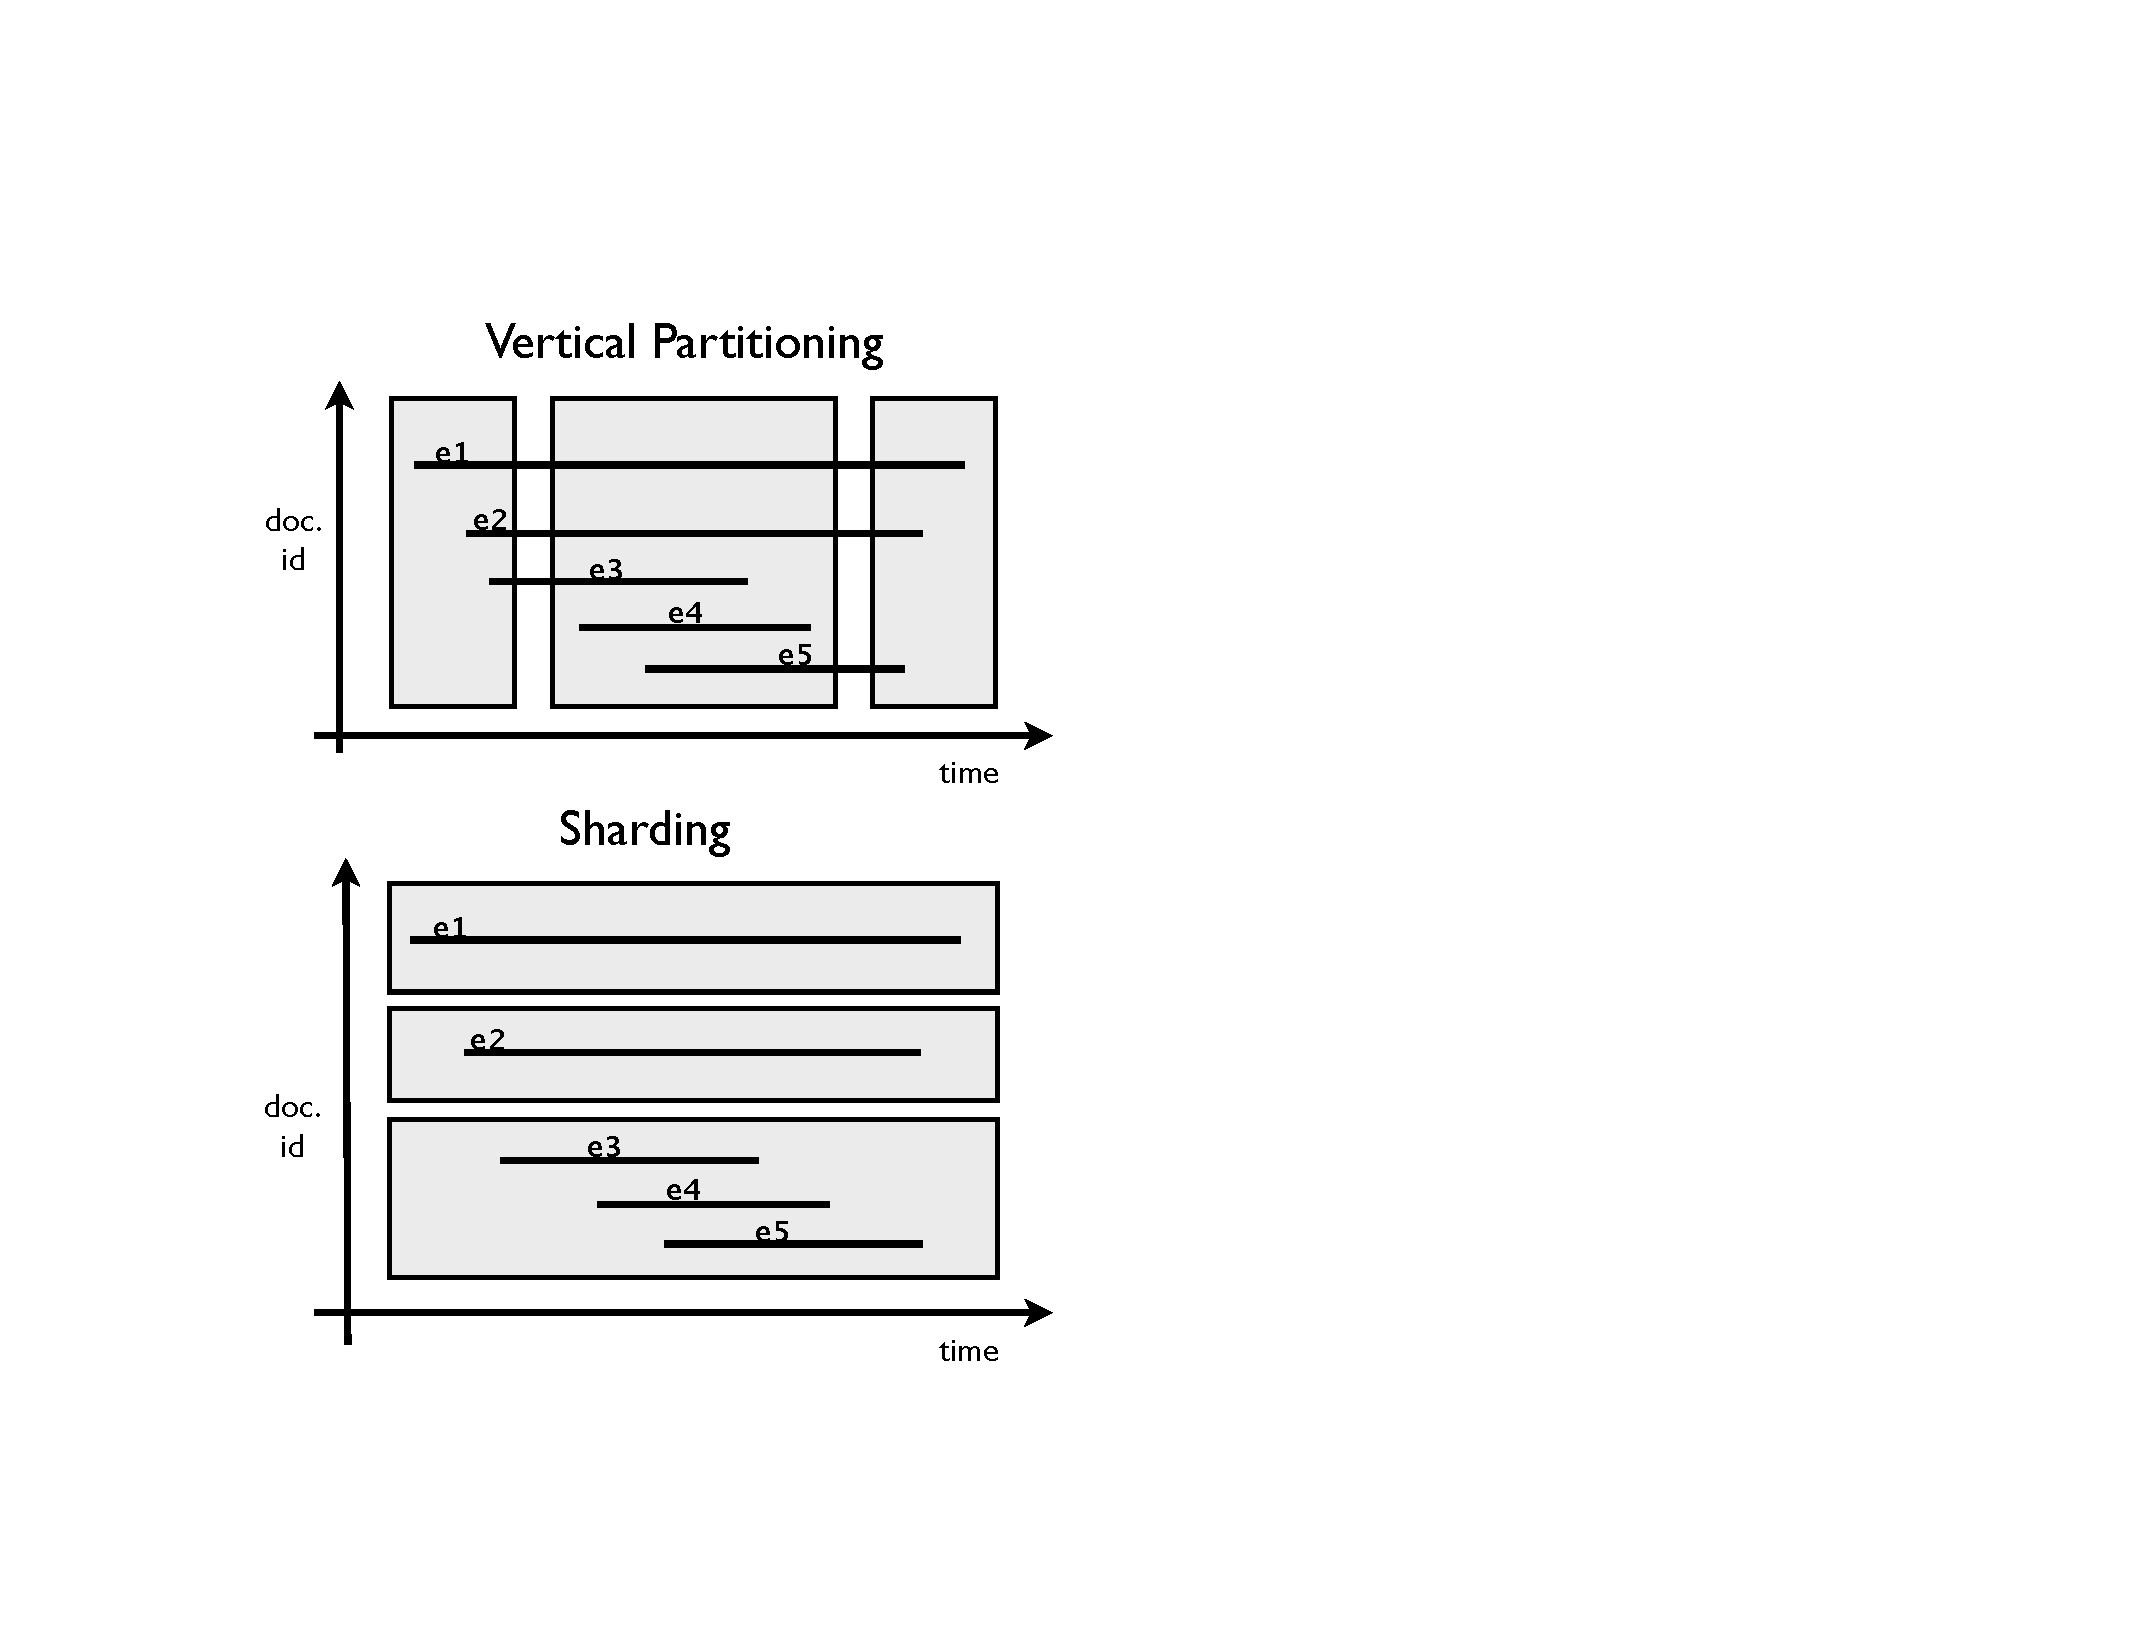
\includegraphics[width=0.6\textwidth]{resources/hor_vs_vert.pdf}
		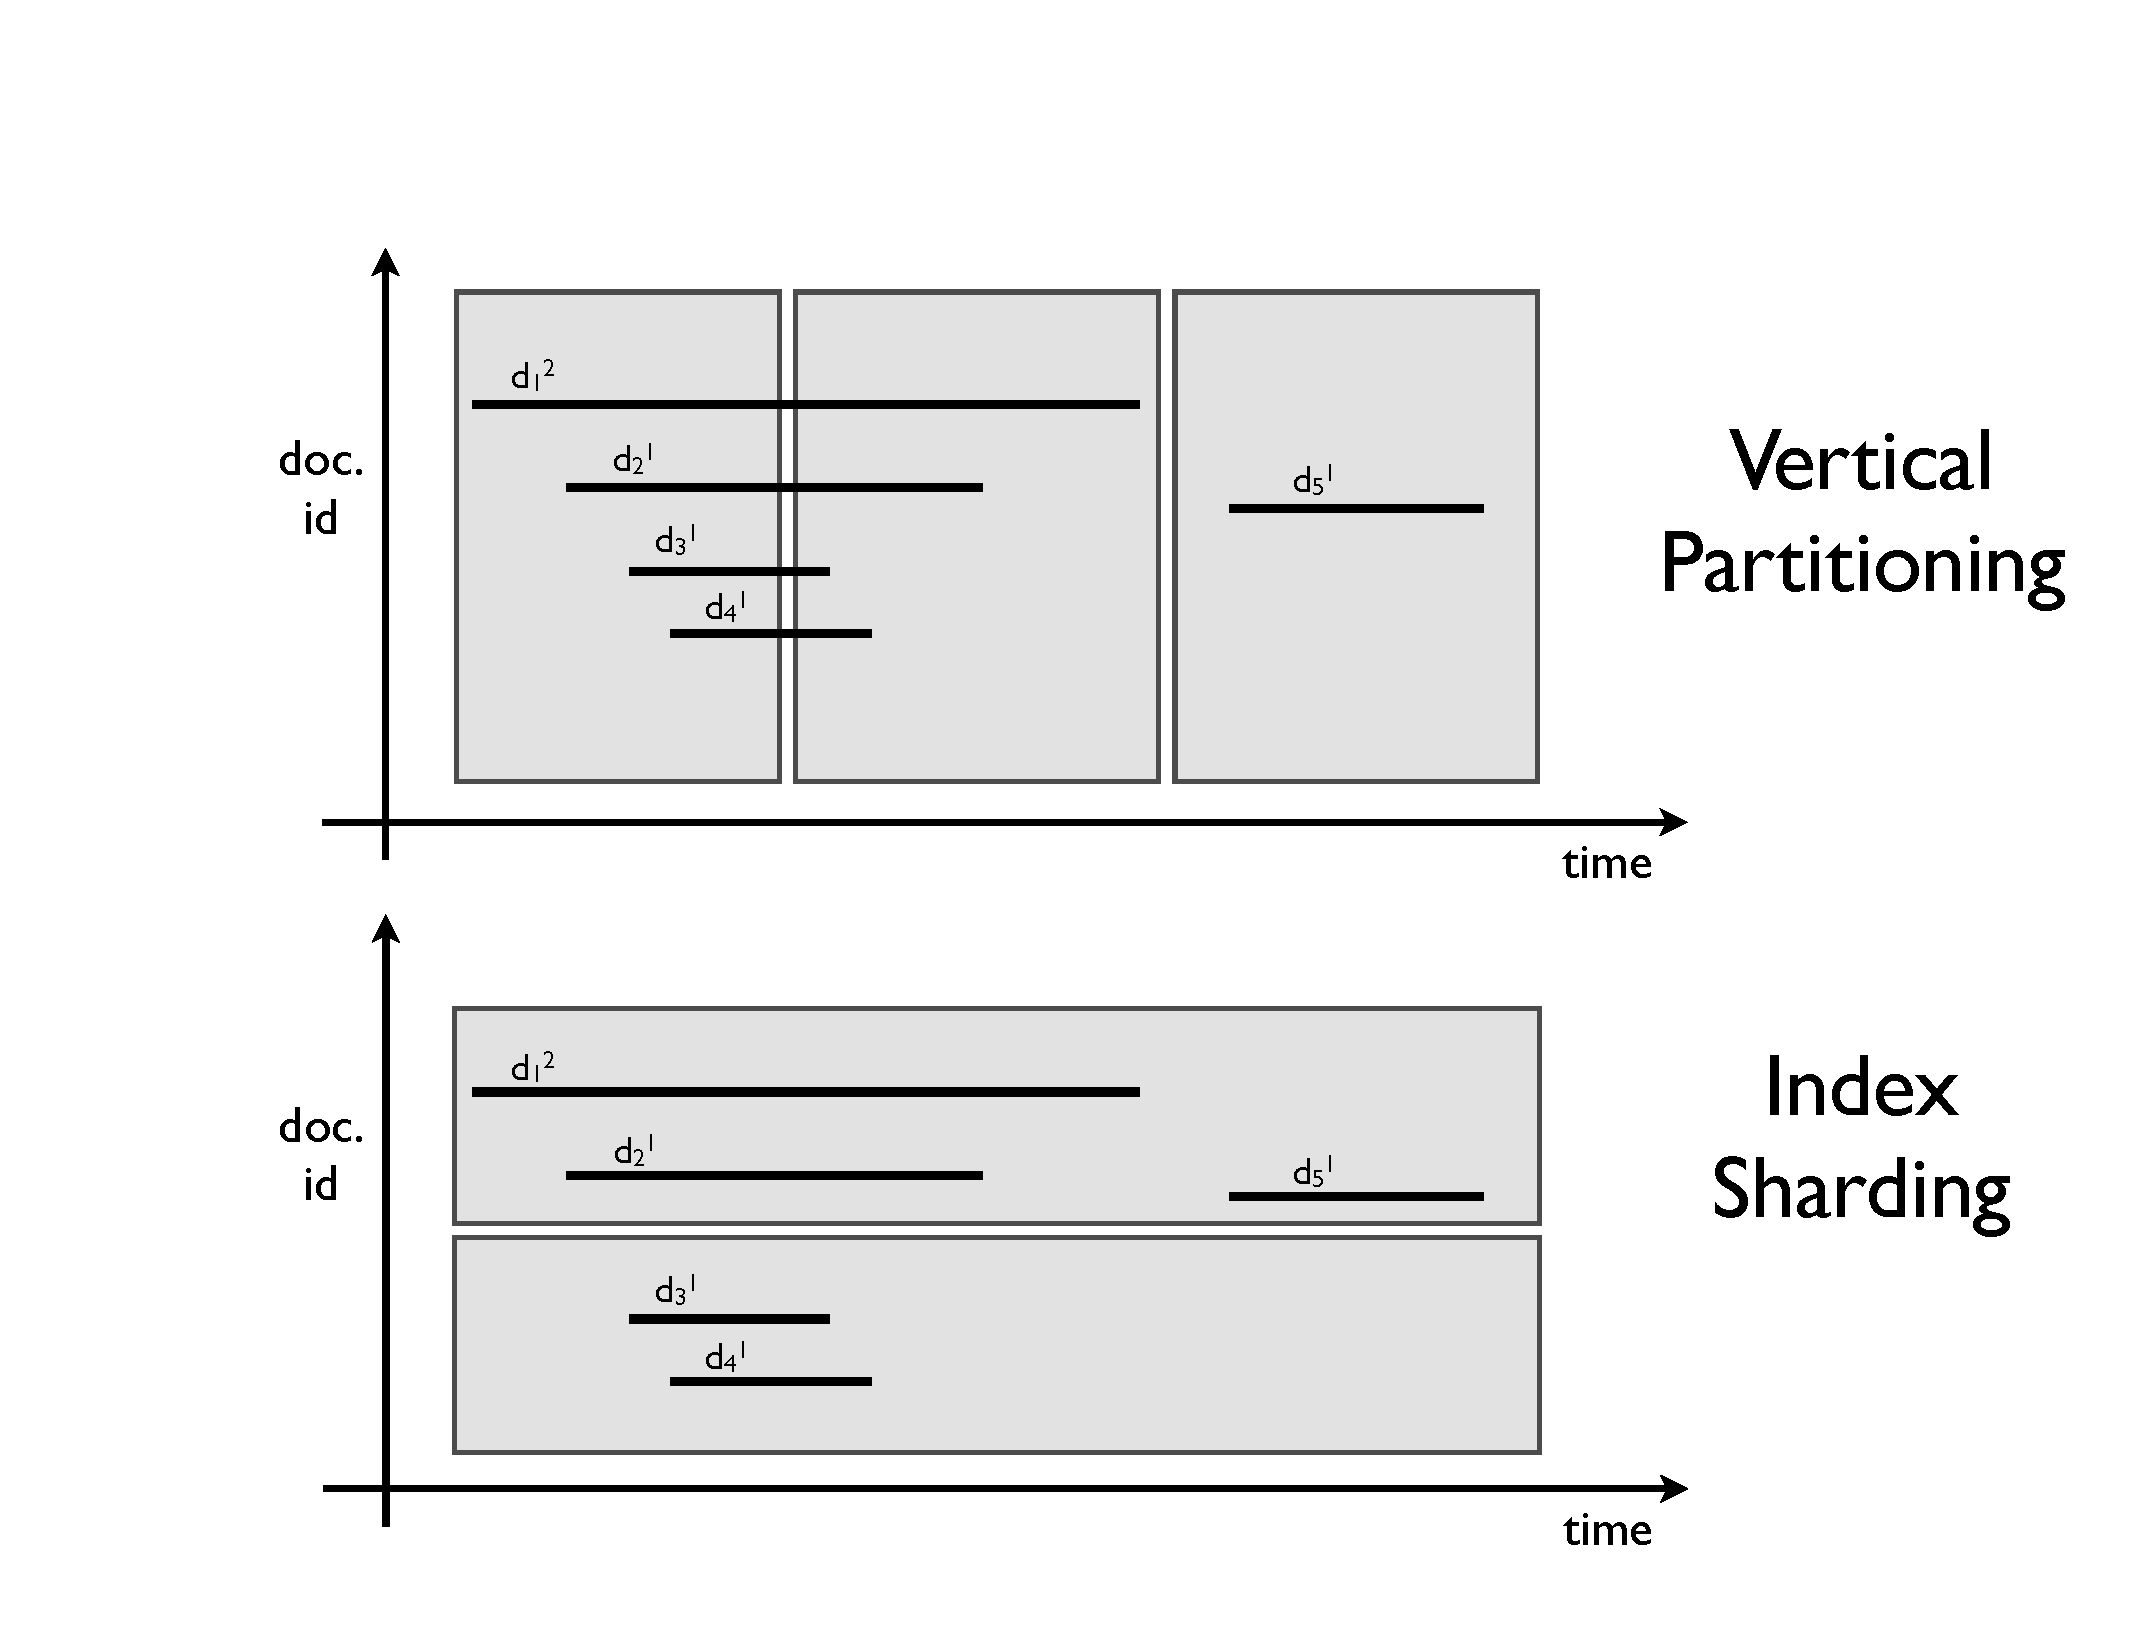
\includegraphics[width=\textwidth]{resources/sharding-vs-vert.pdf}
   	\caption{Vertical partitioning vs. sharding of a posting list}
		  \label{fig:hor_vs_vert}	
\end{figure} 

The state-of-art approaches to process time-travel queries, as discussed in Chapter~\ref{chap:foundations}, transparently extend the inverted index with time-enriched postings. To optimize for time-travel query processing each posting list is partitioned into a number of smaller posting lists along the time dimension. We refer to these methods as \emph{vertical partitioning}. Partitioning in this way reduces access to postings which are irrelevant to the query. Specifically, those postings which do not overlap with the query time-interval. Increasing the degree of vertical partitioning improves the query-processing performance. However, such an index organization suffers from an index-size blowup, incurred due to the replication of postings, due to partitioning. A careful choice of the partitioning boundaries can help to reduce the index-size blowup~\cite{kberberi:sigir2007}, but in order to achieve acceptable levels of efficiency 2 to 3 times index size increase is necessary.

% Answering a time-travel query in such a temporally partitioned index involves choosing the right partition (or partitions) to evaluate the query. 

We look at a novel way of partitioning posting lists called \emph{index sharding} in which we propose to \emph{shard} -- or horizontally partition -- \emph{each posting list} along document identifiers, instead of time (see Figure~\ref{fig:hor_vs_vert}). 
An immediate benefit of this alternative partitioning is almost \emph{no increase} in the overall
index-size (as we show later the only overhead is to maintain a small set of location pointers in each partition). We develop a single-pass
greedy algorithm that optimally shards the posting list, minimizing the
number of postings read during query processing.

The idea is to achieve superior query performance by organizing the postings into shards, exploiting the geometry of the associated intervals, which helps in avoiding access to postings which are irrelevant to the query time-interval. Query processing over a sharded index proceeds by accessing all 
the shards in parallel but reading only a small portion from each of them. As a random access is at least as expensive as a 
sequential read (as in disk-based and network-based index storage), breaking 
the posting list into too many shards actually degrades performance, even if we optimize access to only relevant postings. Thus, the practical 
efficiency of the index organization is achieved only if it is 
sensitive to the cost ratio of random accesses to sequential accesses. 
We formulate optimization problems for tuning the parameter for 
query performance that takes into account the I/O cost ratio of the 
storage infrastructure and propose a heuristic to combine shards to 
gain practical runtime efficiency. 

% In the resulting sharded index, query processing proceeds by first
% \emph{opening} all posting list shards for Xeoneach query term, and
% \emph{seeking} to the right position inside each shard, and, next,
% sequentially scanning the shard from that position --resulting in one
% random access followed by a sequential scan. 

% The first approach relaxes the \textit{shards}, taking into account the I/O characteristics of the storage infrastructure, encoded as a parameter $\eta$ reflecting the cost ratio between random seeks and sequential reads. The method guarantees for every \textit{relaxed shard} that the \textit{expected number} of wastefully read postings is bounded by $\eta$. 

% In the second approach we also get more stringent and consider the worst case by bounding the \textit{maximum number} of wastefully read postings instead. This allows us to develop an online incremental sharding
% algorithm that keeps only a small in-memory buffer for every shard in
% the index. We show that our online algorithm is within an
% approximation factor of $(2 - \frac{2}{\eta + 2})$ and hence results
% in at most two times the optimal number of relaxed shards. This method of sharding serves as the foundation for our update story.
Based on the index sharding principle, we propose a framework which efficiently handles additions of new document versions to the
archive without sacrificing query efficiency. We propose an algorithm which is incremental in nature thus avoiding the expensive recomputation of shards. Further, it reconciles the relative cost of random and sequential access for better query performance. 
%\aanand{is it clear..or long wounded ? is it understandable ?}

% In this approach we distinguish between \textit{active versions}, as the most recent and still current document versions, and \textit{archive versions}, as the document versions already superseded by a more recent version of the same document. To search the active versions, a standard incrementally updatable inverted index~\cite{Buttcher:2008fk,Lester:2008qf} is employed. A detailed discussed can be found in Chapter~\ref{chap:foundations}. Our focus instead is on searching the archive versions. We propose an incremental approach maintaining shards when document versions are superseded and thus need to be migrated from the active index.

\subsection{Contributions}
In summary, the key contributions made in this chapter are the following.

\begin{enumerate}
%\begin{compactenum}
	\item A novel sharded index organization for a
	  time-enriched inverted index that overcomes the issue of
	  index-size blowup.

	\item An optimal greedy algorithm to shard the posting list, so that no time-travel query reads more than the required postings, thus achieving ideal query-processing performance.

	\item A framework that achieves practical runtime efficiency by tuning the number of shards that each posting list is split into, taking into
	  account the I/O cost ratio of the storage infrastructure. Note
	  that the cost of such a partitioning is \emph{independent} of the dynamics in the
	  query workload, as it depends only on the storage system parameters.

    \item A framework to support updates and perform efficient index maintenance based on an incremental sharding algorithm.

    \item An extensive empirical evaluation on large-scale versioned
	document collections using real-world keyword queries with temporal constraints at varying granularities. 

\end{enumerate}

\subsection{Organization}
The remainder of this chapter is organized as follows: In
Section~\ref{chap:sharding:sec:model}, we present the data model 
and index organization that we use in this chapter. Next, in 
Section~\ref{chap:sharding:chap:horizontal_partitioning}, we describe in detail the idea of 
sharding the inverted index and how queries can be processed over the sharded 
index. In Section~\ref{chap:sharding:sec:ideal_part} and in 
Section~\ref{chap:sharding:sec:relaxed_part} we present the details of our idealized sharding and 
a shard-merging strategy. 
Section~\ref{chap:sharding:sec:inc_sharding} describes our incremental sharding method for 
index maintenance. Section~\ref{chap:sharding:sec:system} presents the overall 
architecture of our update-aware retrieval system. Details of our 
experimental setup and its results are presented in Section~\ref{chap:sharding:sec:expt}. 
Finally, we discuss previous related work in Section~\ref{chap:sharding:sec:related}, 
before summarizing in Section~\ref{chap:sharding:sec:summary}.


\section{Model and Index Organization}
\label{chap:sharding:sec:model}
%\index{Index Sharding}


We adopt the document, collection, and query models from Chapter~\ref{chap:foundations} and briefly recap the notation in Table~\ref{tab:sharding_notation}.

\begin{table}
\centering
\begin{tabular}{ll}
\hline  
\multicolumn{1}{l}{\emph{Notation}} &  \multicolumn{1}{l}{\emph{Description}} \\
\hline
$\mathcal{D}$ & collection of documents\\
$\mathcal{V}$ & \emph{vocabulary}, a set of words\\
$d_i^j \in \mathcal{D}$ & a document version, $j^{th}$ version of document $d_i$\\
$valid(d_i^j)$ & valid-time interval \\ 
$begin(d_i^j)$ & begin time of $d_i^j$  \\
$end(d_i^j)$ & end time of $d_i^j$ \\
$Q$ & time-travel query\\
$keywords(Q)$ & set of keywords in $Q$\\
$interval(Q)$ & query time-interval of $Q$\\
$I_1 \overlaps I_2$ & Overlapping intervals $I_1$ and $I_2$ \\
$I_1 \noverlaps I_2$ & Non-overlapping intervals $I_1$ and $I_2$ \\
\hline
\end{tabular}
\caption{Notation}
\label{tab:sharding_notation}
\end{table}

We call a document version $d_i^k$ an \emph{active version} if it is the most current version of document $d_i$ and consequently has $end(d_i^k) = \infty$ where the current time or ``now'' is represented as $\infty$. 

Our proposed index for time-travel queries is based on the
established \emph{inverted index} as described in Chapter~\ref{chap:foundations}. We extend the inverted index to support 
time-travel queries by modifications to the postings structure, 
posting-list organization, and the lexicon. 


We extend the contents of each posting by additionally storing the valid-time 
interval, $valid(d_i^k) = [begin(d_i^k), end(d_i^k))$, of the document version $d_i^{k}$
along with the identifier $d_i$, and a payload $s$, i.e.,
$$\langle d_i^k, [ begin(d_i^k), end(d_i^k)], s\rangle.$$

The index organization supports different retrieval models by allowing the
payloads to be empty (for Boolean retrieval), containing a scalar value ($tf$ in the document
version) or containing positional information (phrase-based retrieval). When no confusion
arises, we simply use $begin(p)$ and $end(p)$ of a posting $p$ to
refer to the valid-time interval boundaries of the corresponding document version.

%index organization
We partition each posting list into disjoint 
partitions referred to as \emph{shards}. The postings in a shard are ordered 
according to their begin times. We assign the identifiers to documents
and versions in the order of their begin times. This ensures that the postings are also
 ordered by their identifiers in a shard. Subsequently we can use standard compression 
  techniques, commonly used for posting-list compression, for compressing shards. 

%lexicon
As a result of index sharding, each term in the vocabulary may be associated
with multiple lists. These mappings have to be appropriately reflected in the lexicon. 
To this end, we extend the lexicon to store pointers 
to all the shards for each term. Note that since our partitions are not local to a given time interval we 
do not need to maintain time intervals corresponding to each partition, 
unlike the lexicon of the vertically-partitioned index.


\begin{figure}[tb]
	\centering
		%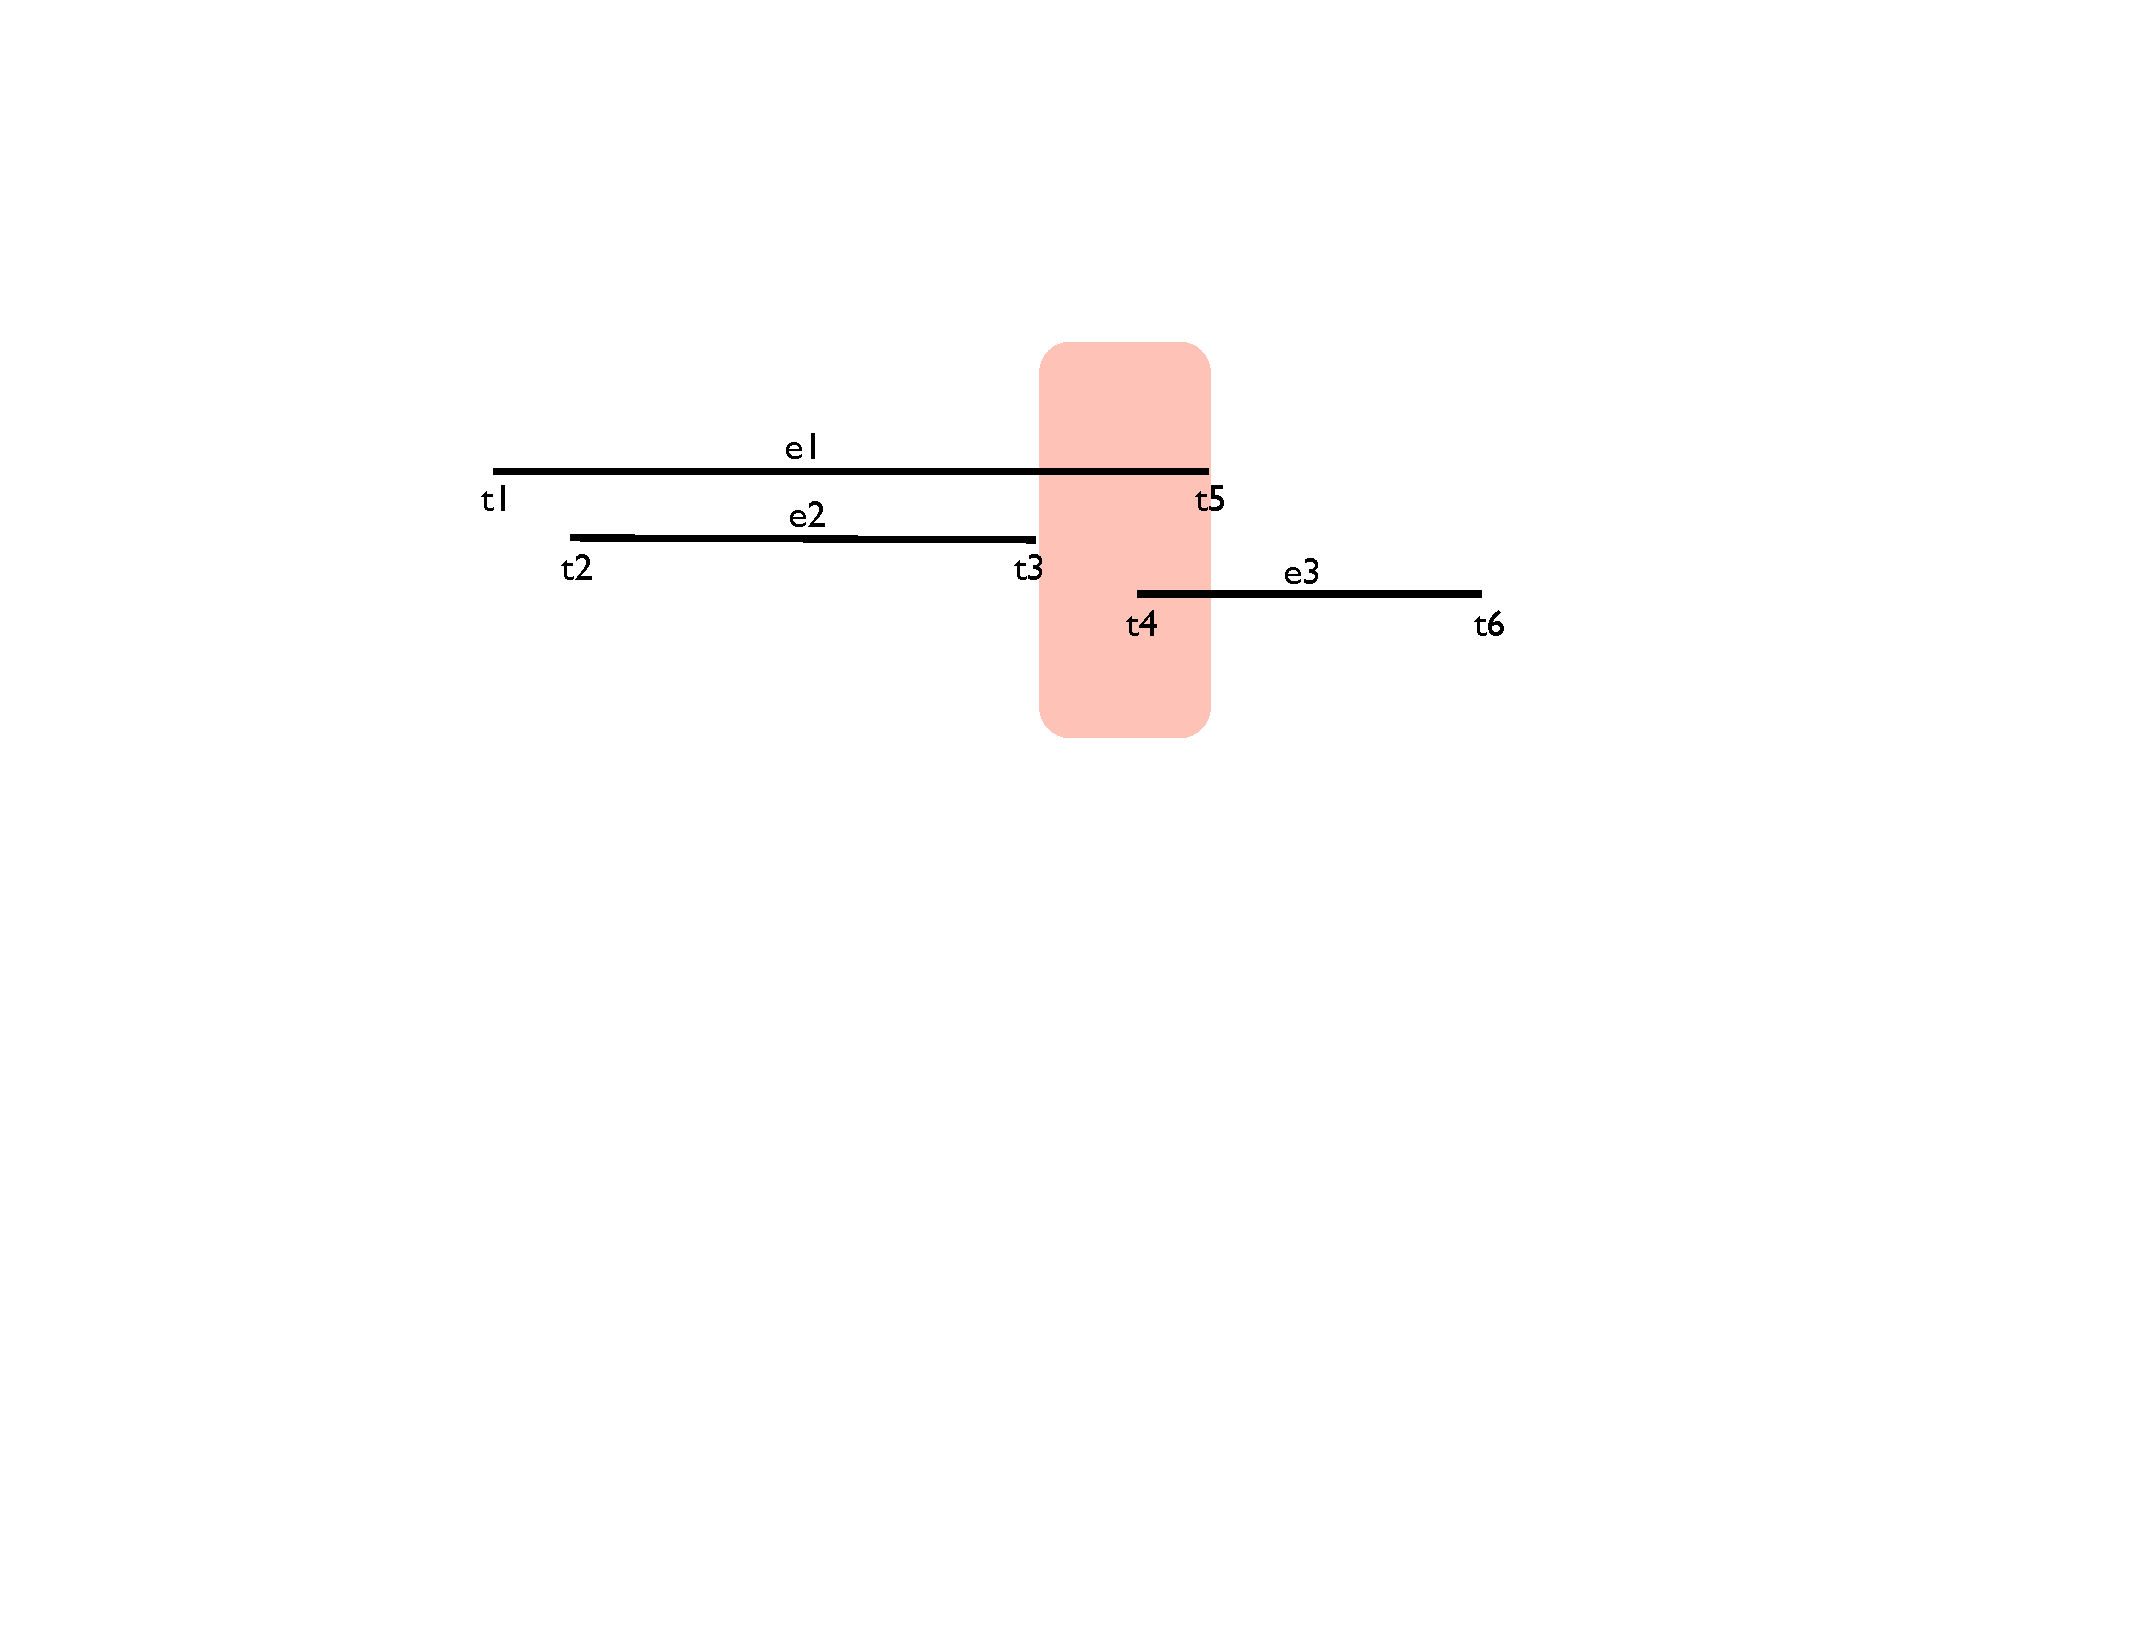
\includegraphics[width=0.6\textwidth]{resources/qp_relaxed.pdf}
		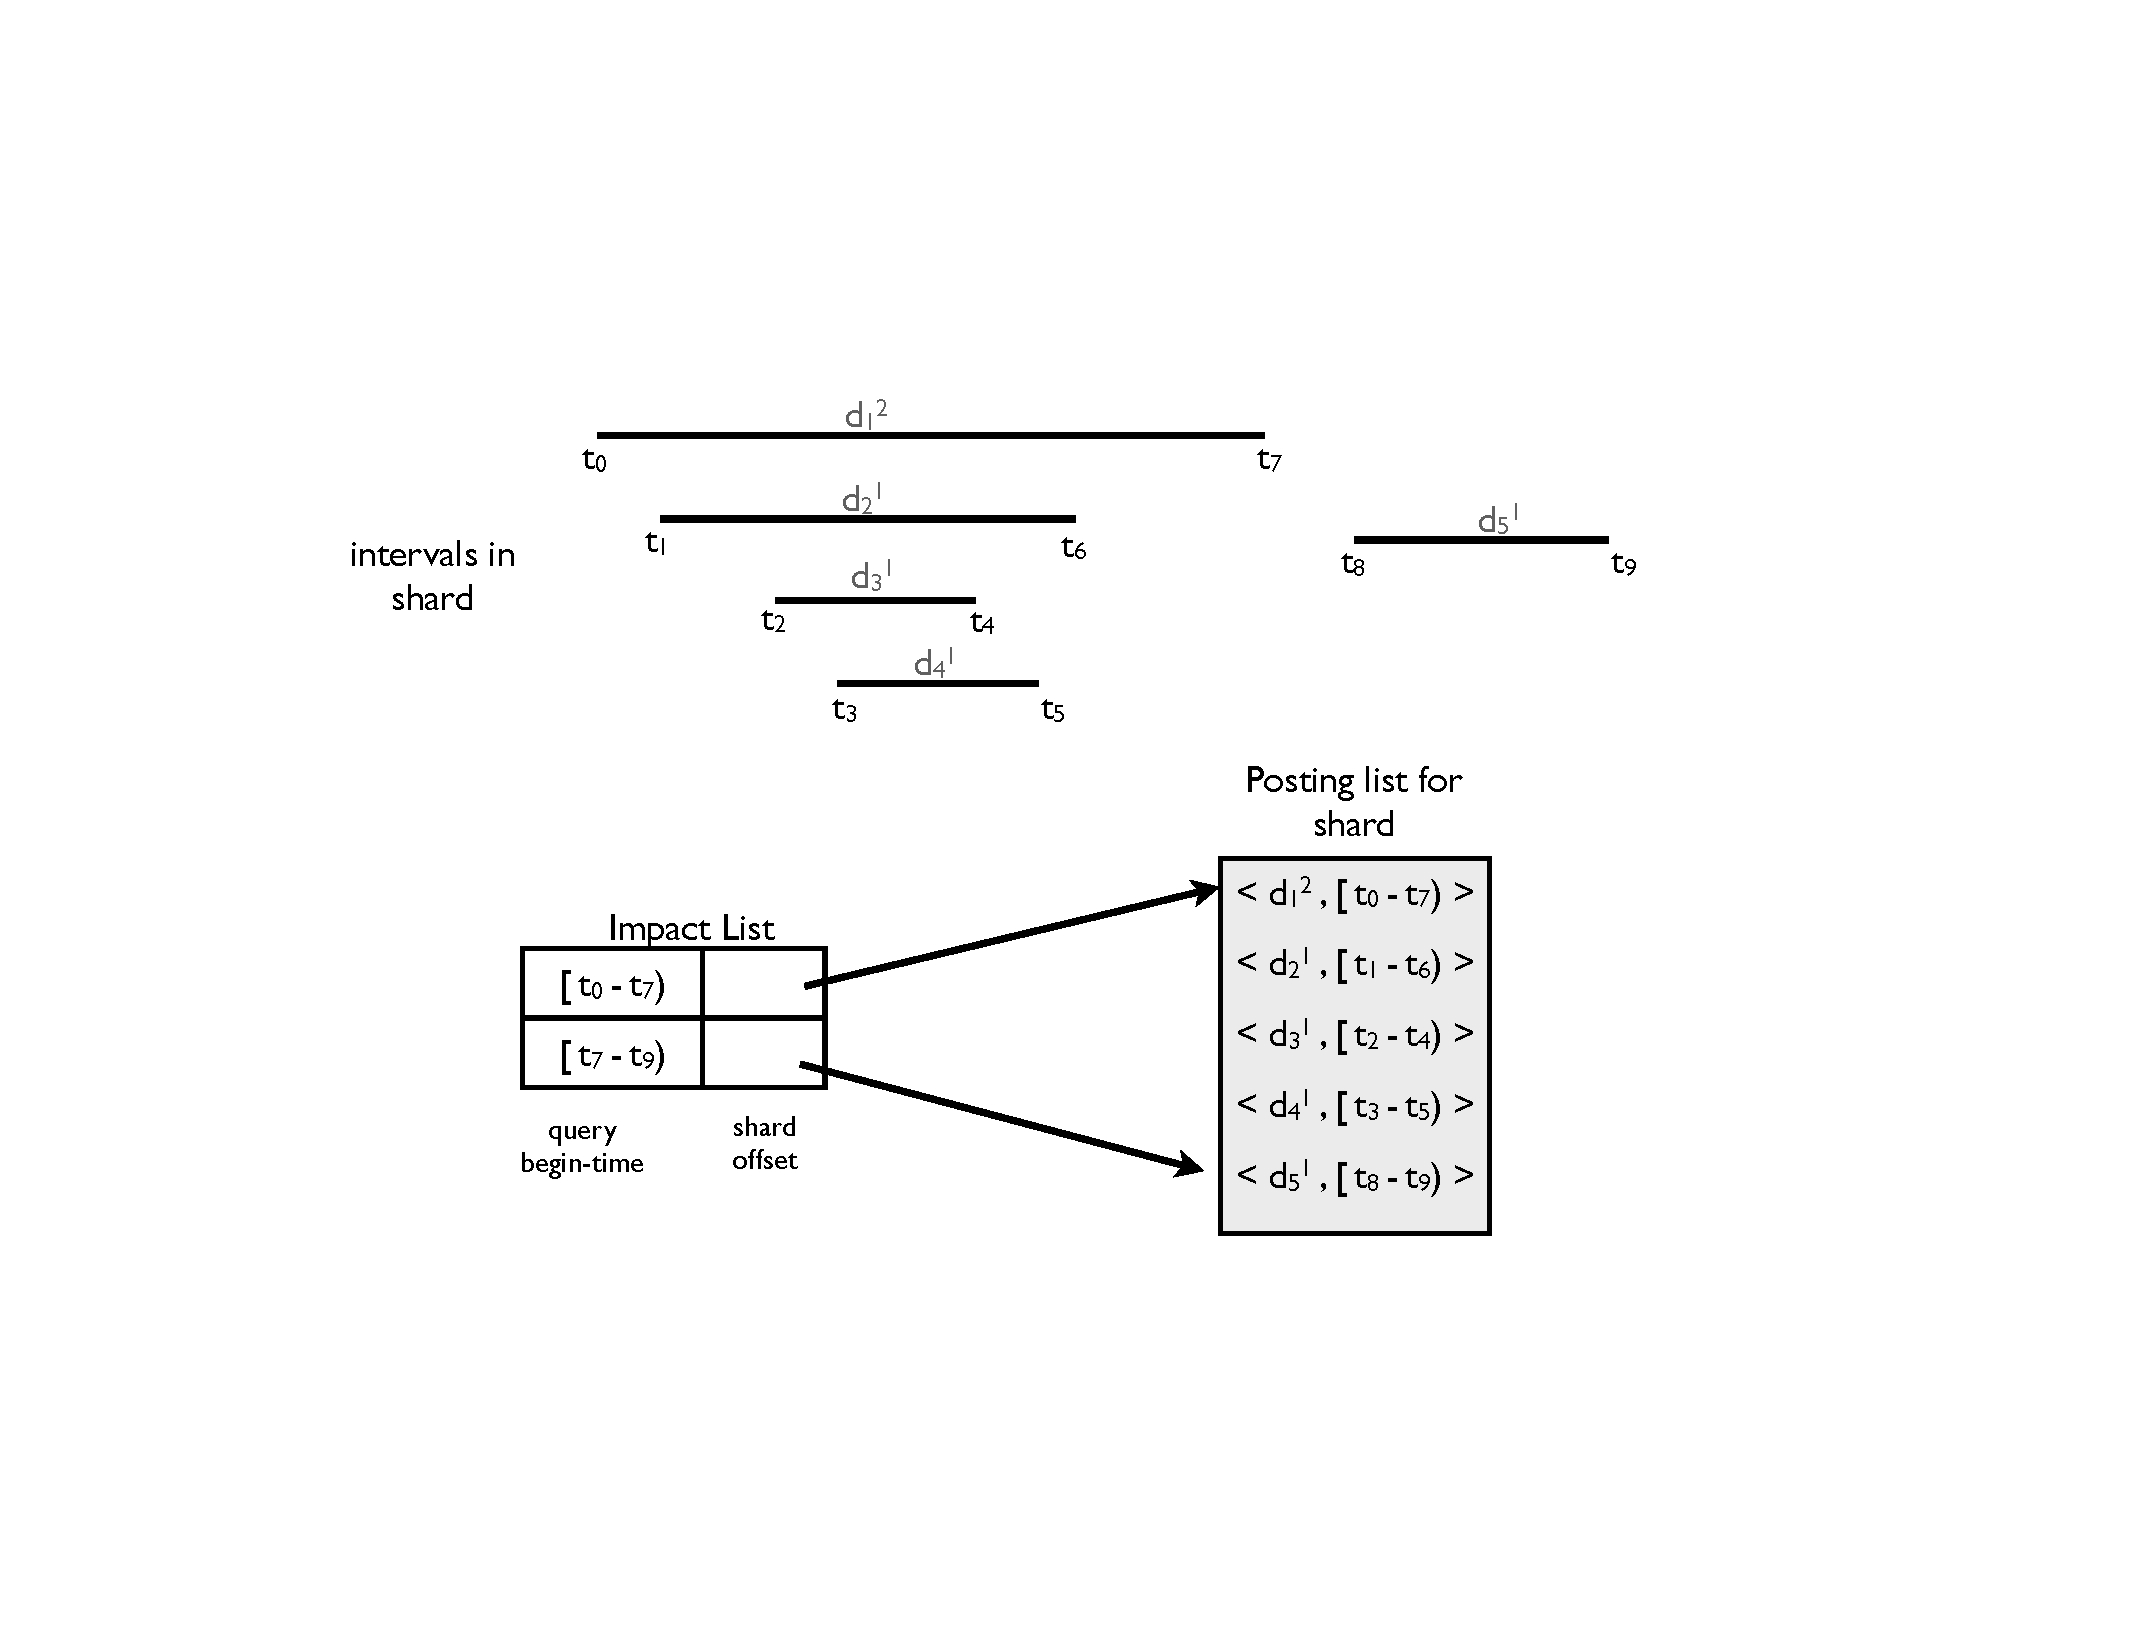
\includegraphics[width=\textwidth]{resources/impact-list.pdf}
	\caption{Impact list}
	 \label{fig:impactlist}
\end{figure}


%impact list
\paragraph{Impact Lists} For each shard we maintain an additional access structure for efficiently determining the postings whose time intervals overlap with a query time-interval. These are called \emph{impact lists}. An impact list is an associative data structure which maintains, for every possible begin time of a query time-interval, the position in
the shard of the earliest posting whose valid time overlaps with the query begin time. In other words, the impact list stores pairs of query begin times (key) and offsets (values) from the shard beginning. The overall size of each impact list can be reduced by storing only the distinct offset values rather than offsets for all possible query begin times. An example of an impact list of a shard of five postings is shown in Figure~\ref{fig:impactlist}. The possible begin times are represented as intervals and they map to the offset in the posting list for the shard from where the postings are read sequentially. Thus, for a query interval in $[t_8 - t_{11}]$ we start accessing the list sequentially from the fifth posting. Although represented as intervals, in practice it is sufficient to store the begin or end of the interval. 
Thus keys admit a non-decreasing integer sequence and a straightforward binary search over the keys efficiently gives the correct offset location. For practical granularities of query begin times such as days, the impact lists for the complete index (i.e., for all shards of all terms) can be easily kept in memory. We discuss how query processing is performed using impact lists in the next section.


\section{Sharding Posting Lists} 
\label{chap:sharding:chap:horizontal_partitioning}
Index sharding refers to partitioning or sharding a posting list $L_v$ into disjoint partitions or \emph{shards} such that no two shards share common postings. We now formally define the notion of a shard and posting-list sharding. 

\begin{definition}[Shard]
A shard $\sigma$ is a sequence of postings, $\sigma \,=\,\langle p_i\rangle$, ordered by their begin times, i.e., 
$$
	begin(p_i) \leq begin(p_{i+1}).
$$ 
\end{definition}

\begin{definition}[Posting-List Sharding]
Given a posting list $L_{v}$ for a term $v$, posting-list sharding partitions $L_{v}$ into a set of shards $\mathcal{S}_v \,=\, \{\sigma_1, \ldots, \sigma_{m}\}, \, \sigma_{i} \subseteq L_{v}$ where

\begin{equation*}
	\begin{aligned}
		& \left( \forall i,\forall j \; i \neq j \implies \sigma_{i} \cap \sigma_{j} = \emptyset \right) 
		& & \wedge & 
		& \left( \bigcup_{i}{\sigma_i} =  L_{v} \right).  
	\end{aligned}
\end{equation*}

\end{definition}

In what follows a sharded index refers to an index which employs posting-list sharding. A sharded index thus maintains multiple shards per term and the disjoint partitioning avoids replication completely (see Figure~\ref{fig:hor_vs_vert}). 

\subsection{Query Processing over Sharded Index}

For query processing over a sharded index, we employ the established term-at-a-time query-processing 
model (described in more detail in Chapter~\ref{chap:foundations}). In short term-at-a-time processing posting lists are read one after the other and scores of a document version from different lists are merged in memory. For our sharded index, each shard of every query term is processed in a sequence of the following \emph{open-skip-scan} operations.

\begin{figure}[tb]
	\centering
		%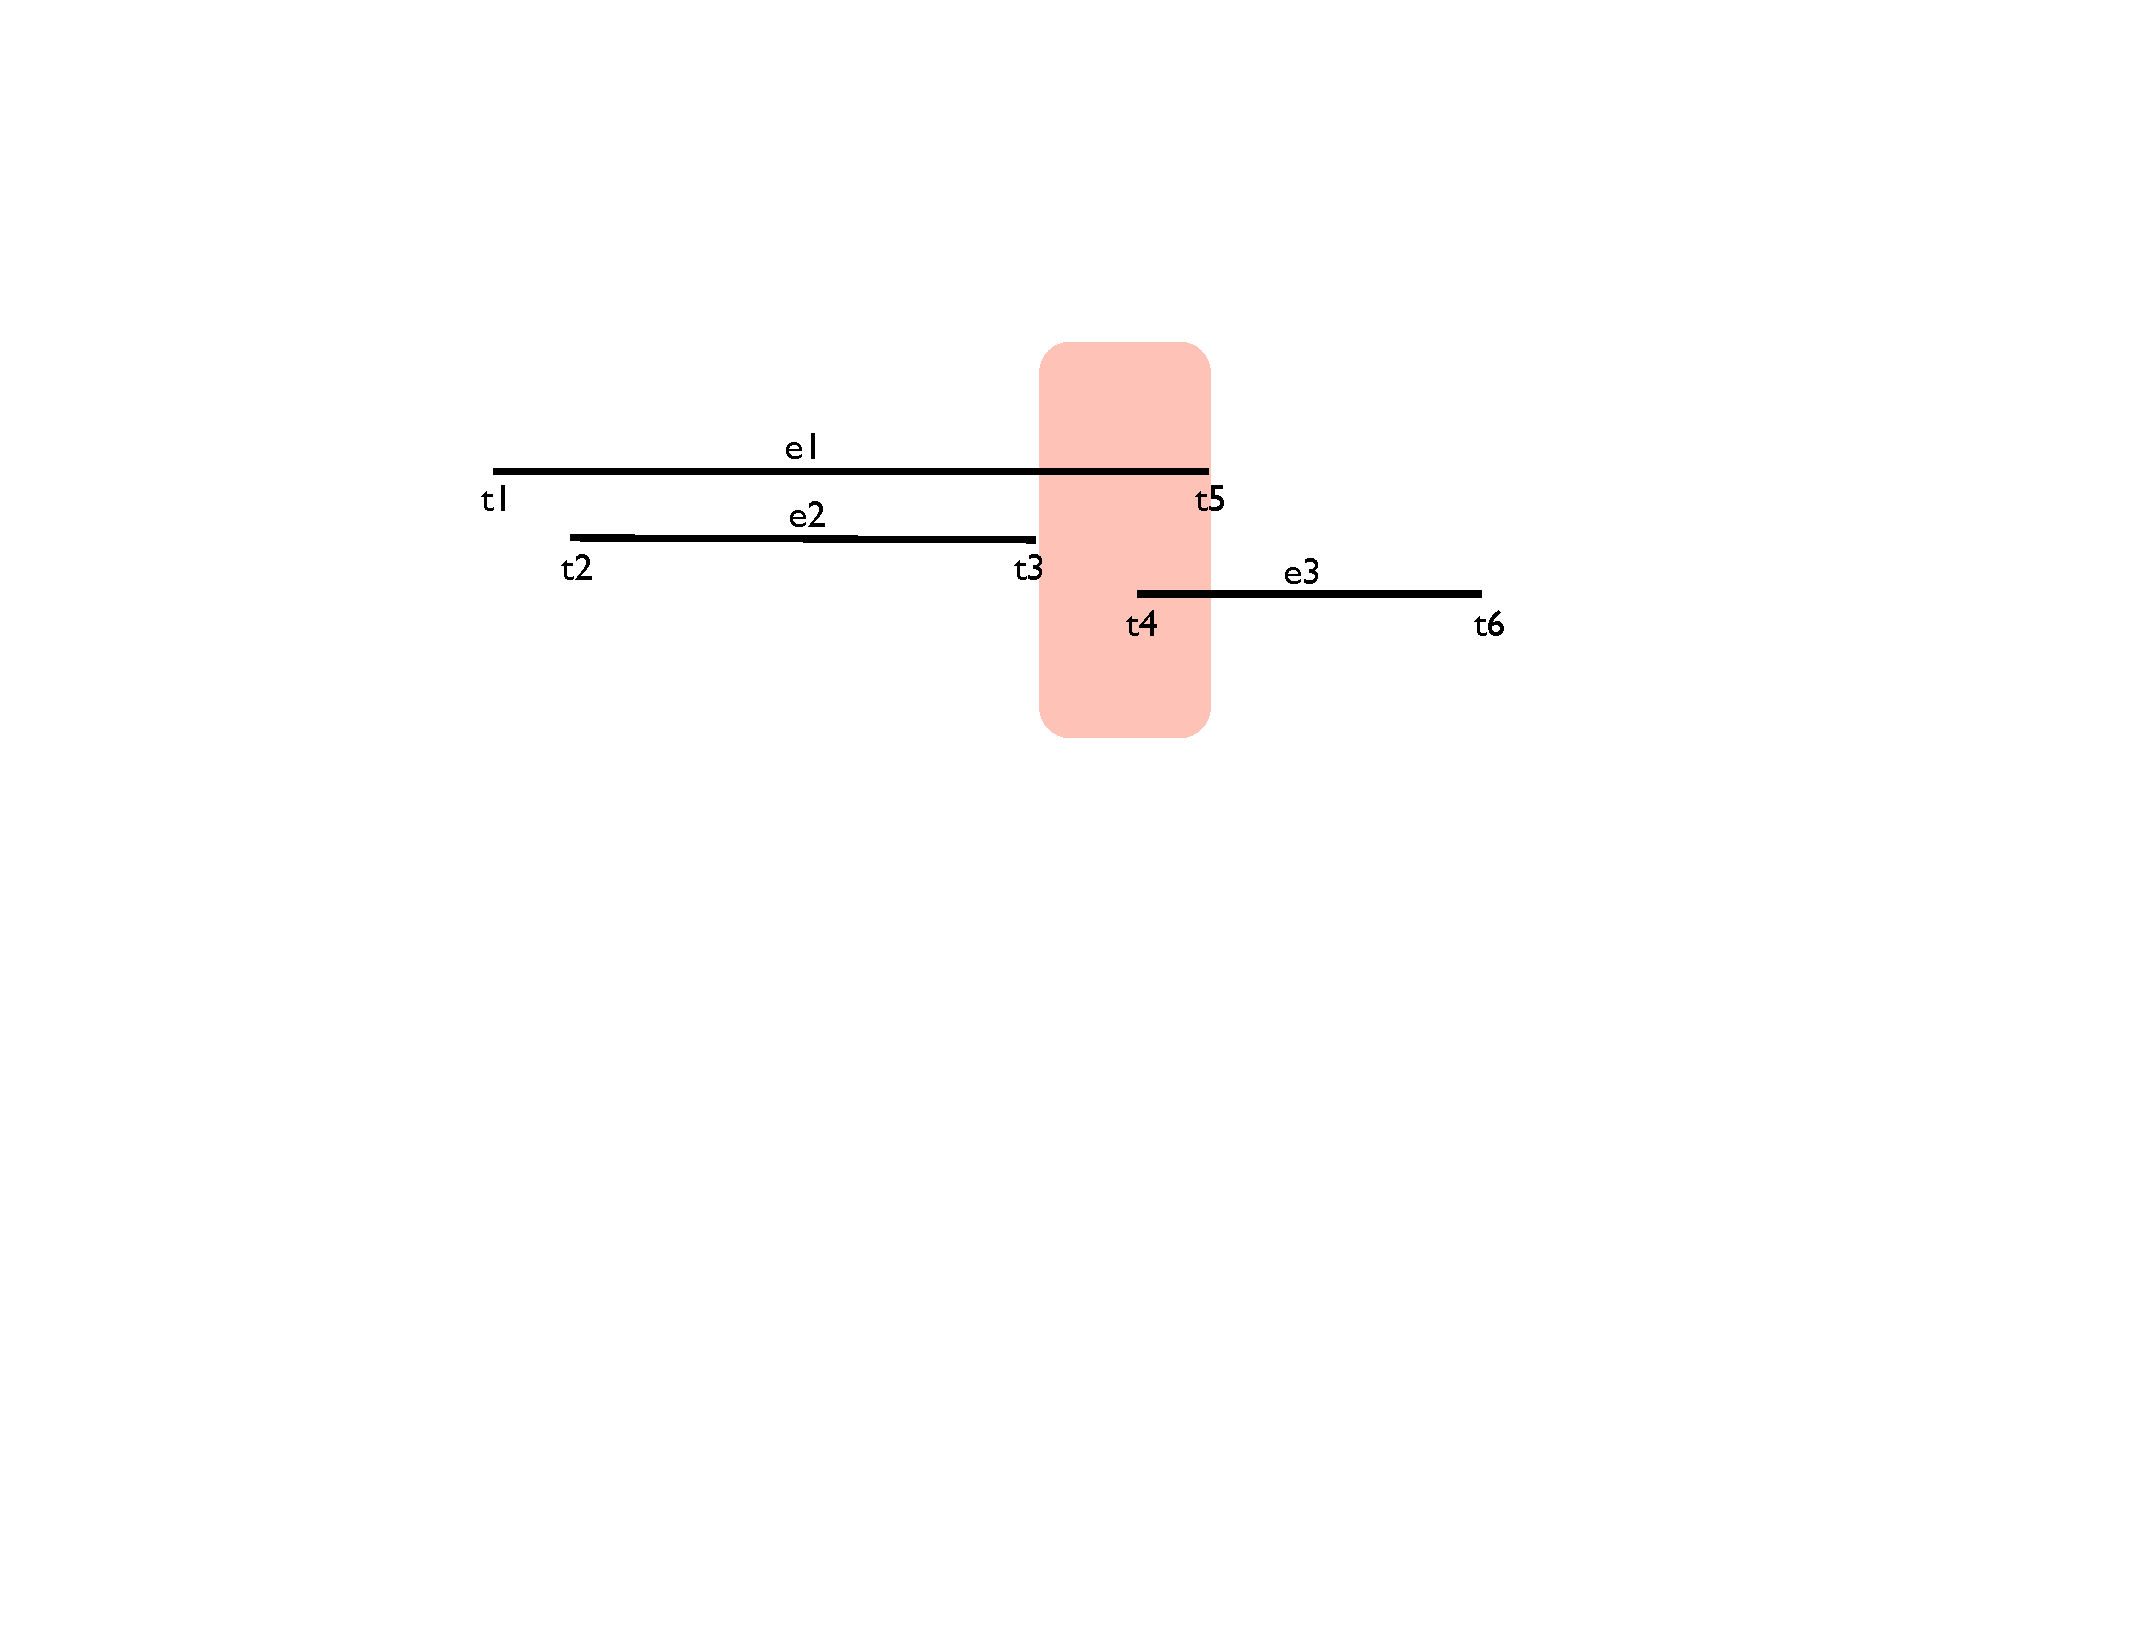
\includegraphics[width=0.6\textwidth]{resources/qp_relaxed.pdf}
		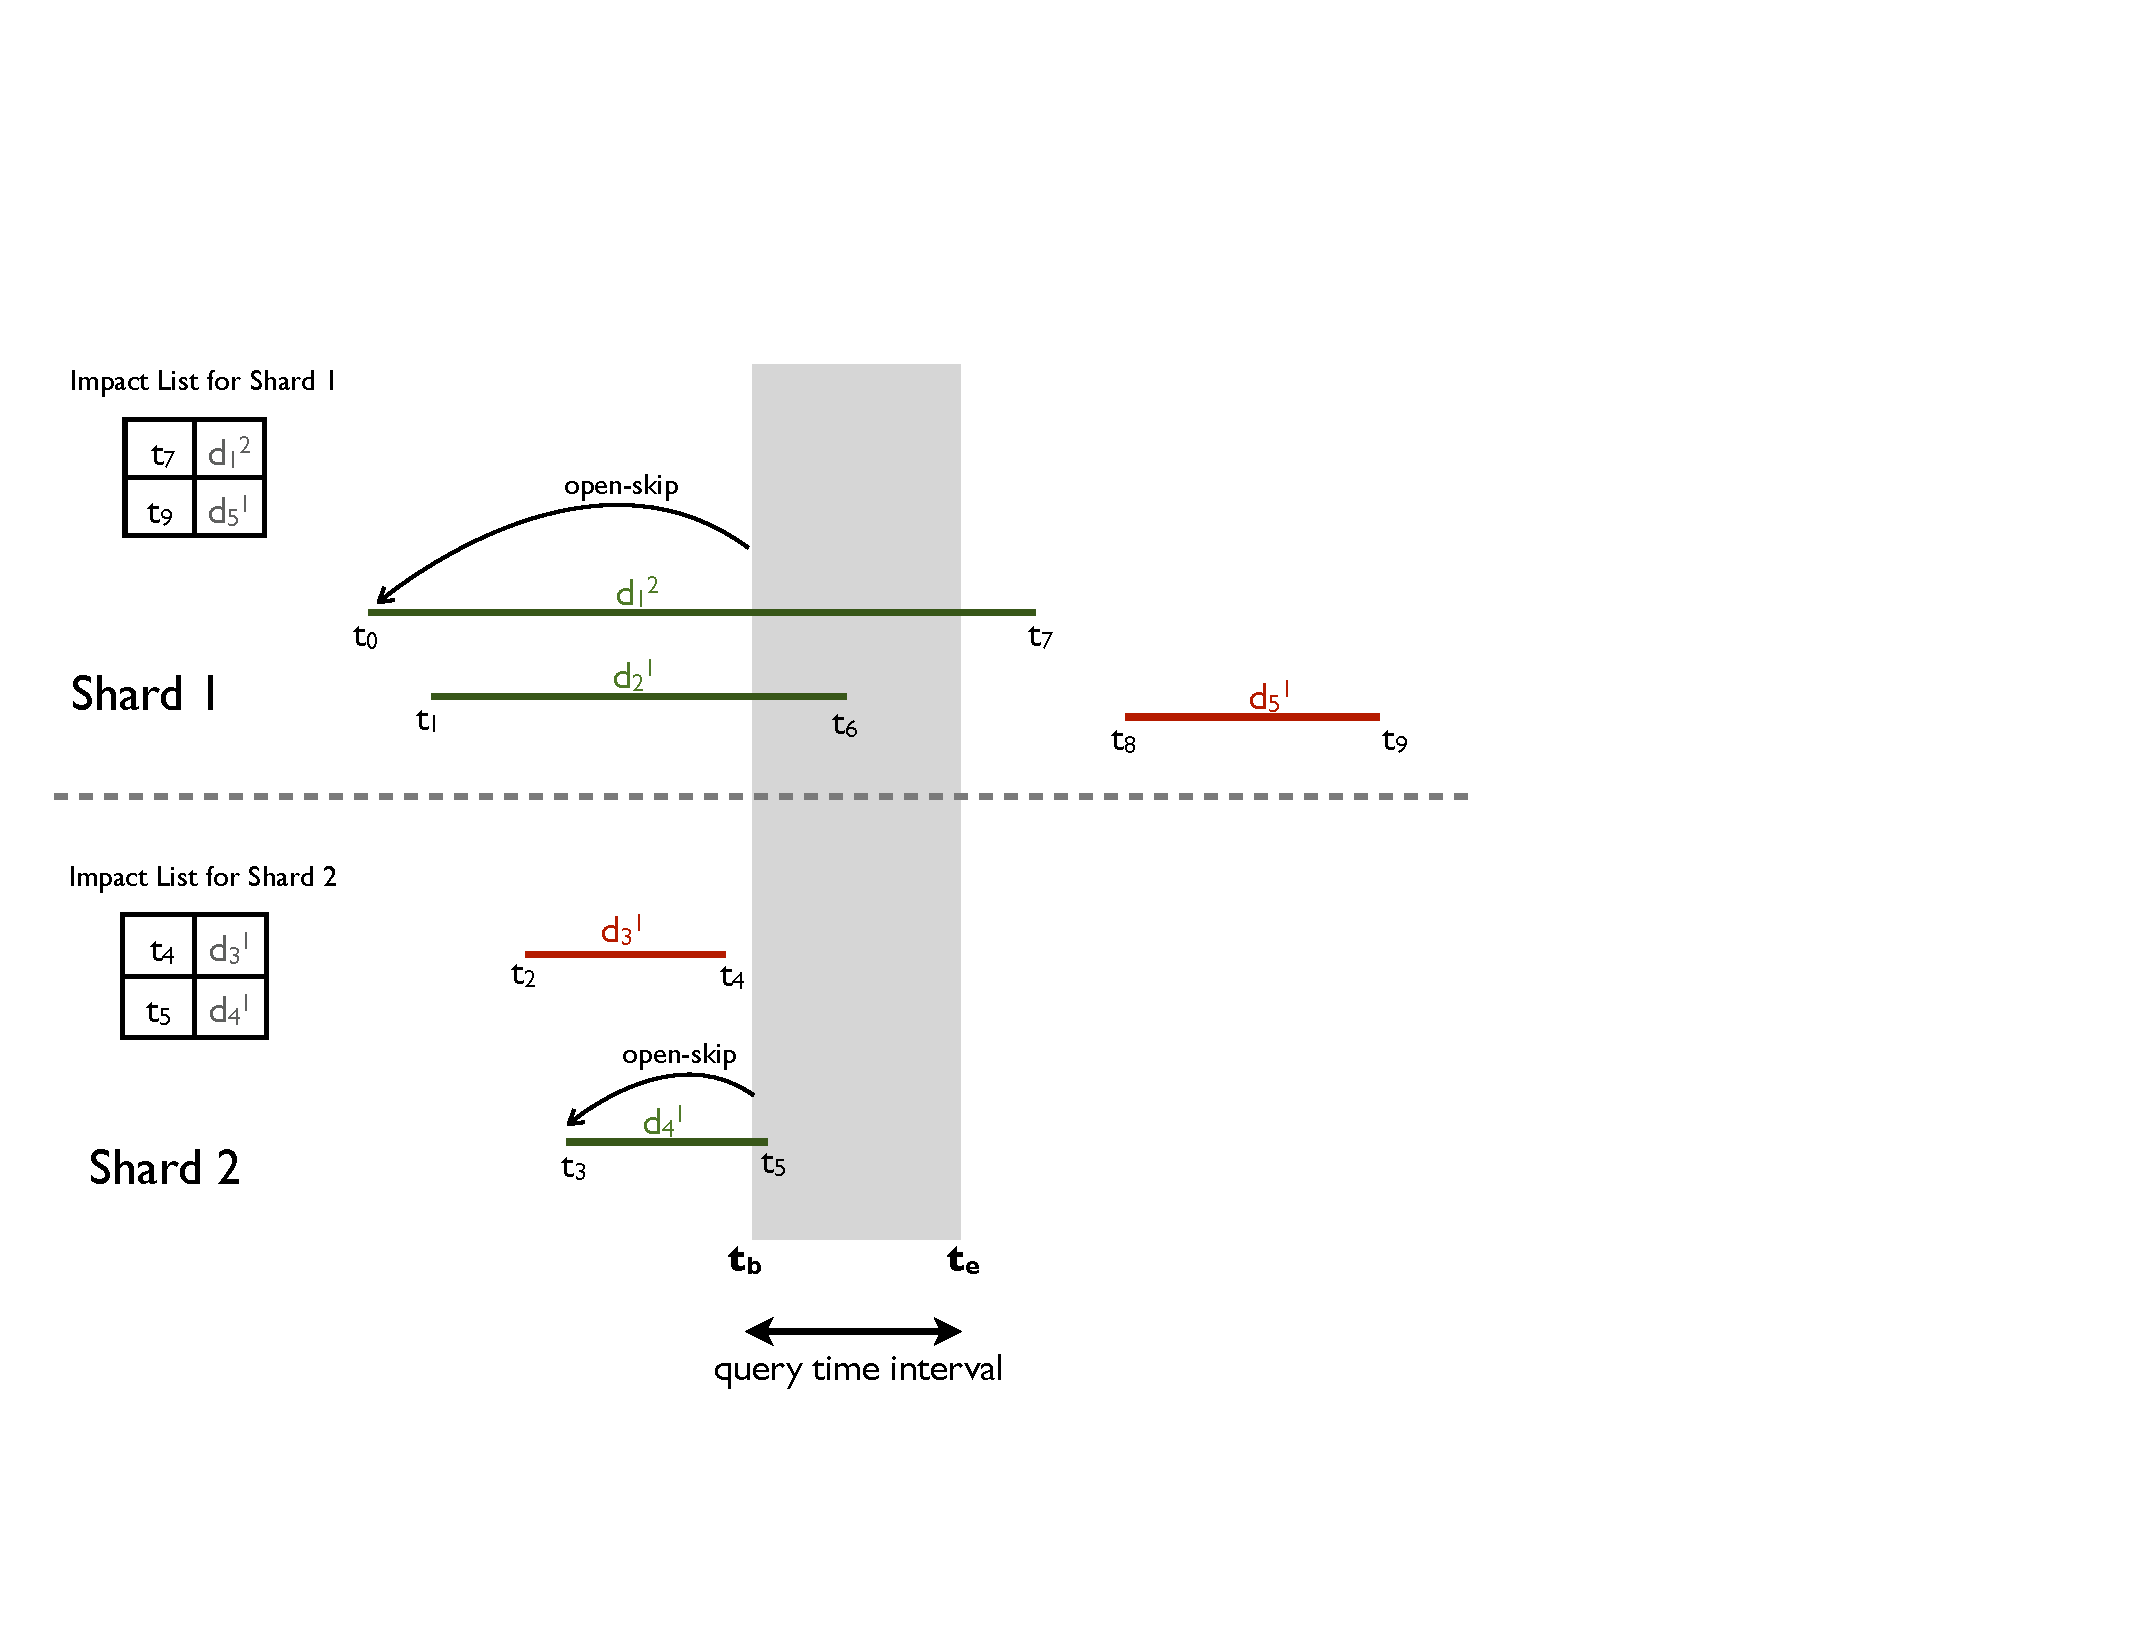
\includegraphics[width=\textwidth]{resources/qp_shards.pdf}
	\caption{Open-skip and scan operations for query processing}
	 \label{fig:open-skip-scan}
\end{figure}

\begin{enumerate}
\item \textbf{Open} -- Open a shard for a query term. This involves a lookup from the lexicon for the location of beginning of the shard.

\item \textbf{Skip} -- Given the query begin time, lookup offset 
position from the impact list of the shard and perform a seek to that 
position. In practice we can combine the open and skip steps into an
\emph{open-skip} operation to avoid an extra I/O operation. 

\item \textbf{Scan} -- Perform sequential reads from this position and
  terminate when it is certain that the rest of the postings do not overlap
  with the query time-interval. As we read the postings sequentially in
  begin-time order, we can safely terminate when the begin time of the
  next posting exceeds the query end-time.
\end{enumerate}

An illustration of the query-processing operation is shown in Figure~\ref{fig:open-skip-scan}. We are given a sharding $\seq{ d_1^2, d_2^1, d_5^1}$ and $\seq{ d_3^1, d_4^1}$. Each of the shards is associated with an impact list, as illustrated in the figure. For simplicity we denote the offsets from the shard beginning by the posting which is accessed first. 

Consider a time-travel query with time interval $[ t_b, t_e]$, shaded in gray, where we have $ t_3 < t_b < t_4$. Firstly, by the use of impact lists we try to quickly \emph{skip} to the first overlapping posting in the shard. For instance, in the second shard, by looking up the impact list, we start accessing the shard from the second posting onwards. This avoids processing of postings at the head of the shard which do not overlap with the query time-interval. Secondly, the postings are accessed sequentially, from the seek position, until a posting $p$ is encountered such that $begin(p) > t_e$. In the example, we terminate reading Shard 1 after accessing the first two postings and thus avoid reading $d_5^1$.

In essence, we only access a relatively smaller number of postings of a shard. 

For each query, all the participating shards can be processed in parallel. Since the contents postings per shard are disjoint, merging lists is relatively inexpensive. However, if the number of shards per term are large in number, query-processing performance might degrade due to a large number of random seeks (open for each open-seek operation). We now at look at the different posting-list sharding strategies for optimizing query performance.

\section{Idealized Index Sharding}
\label{chap:sharding:sec:ideal_part}

Although the begin-time order in shards avoids wasteful reading of
postings, it does not guarantee the elimination of all wasteful reads. 
A posting is said to be a \emph{wasted read}, if it is accessed during
query processing although its valid-time interval does not overlap
with the query time-interval. We introduce the concept of \emph{subsumption} in shards to explain why this occurs.

\begin{definition}[Subsumption of Postings]
\label{def:staircase}
For a pair of postings $p$ and $q$ (from the same posting list), $p$ subsumes $q$ (for short $p \sqsupset q$) if
$$
p \sqsupset q \Leftrightarrow  \left( begin (p)\leq begin (q) \right) \,\,\wedge \,\, \left( end(p) > end(q) \right).
$$ 
\end{definition}

\begin{figure}[tb]
	\centering
		%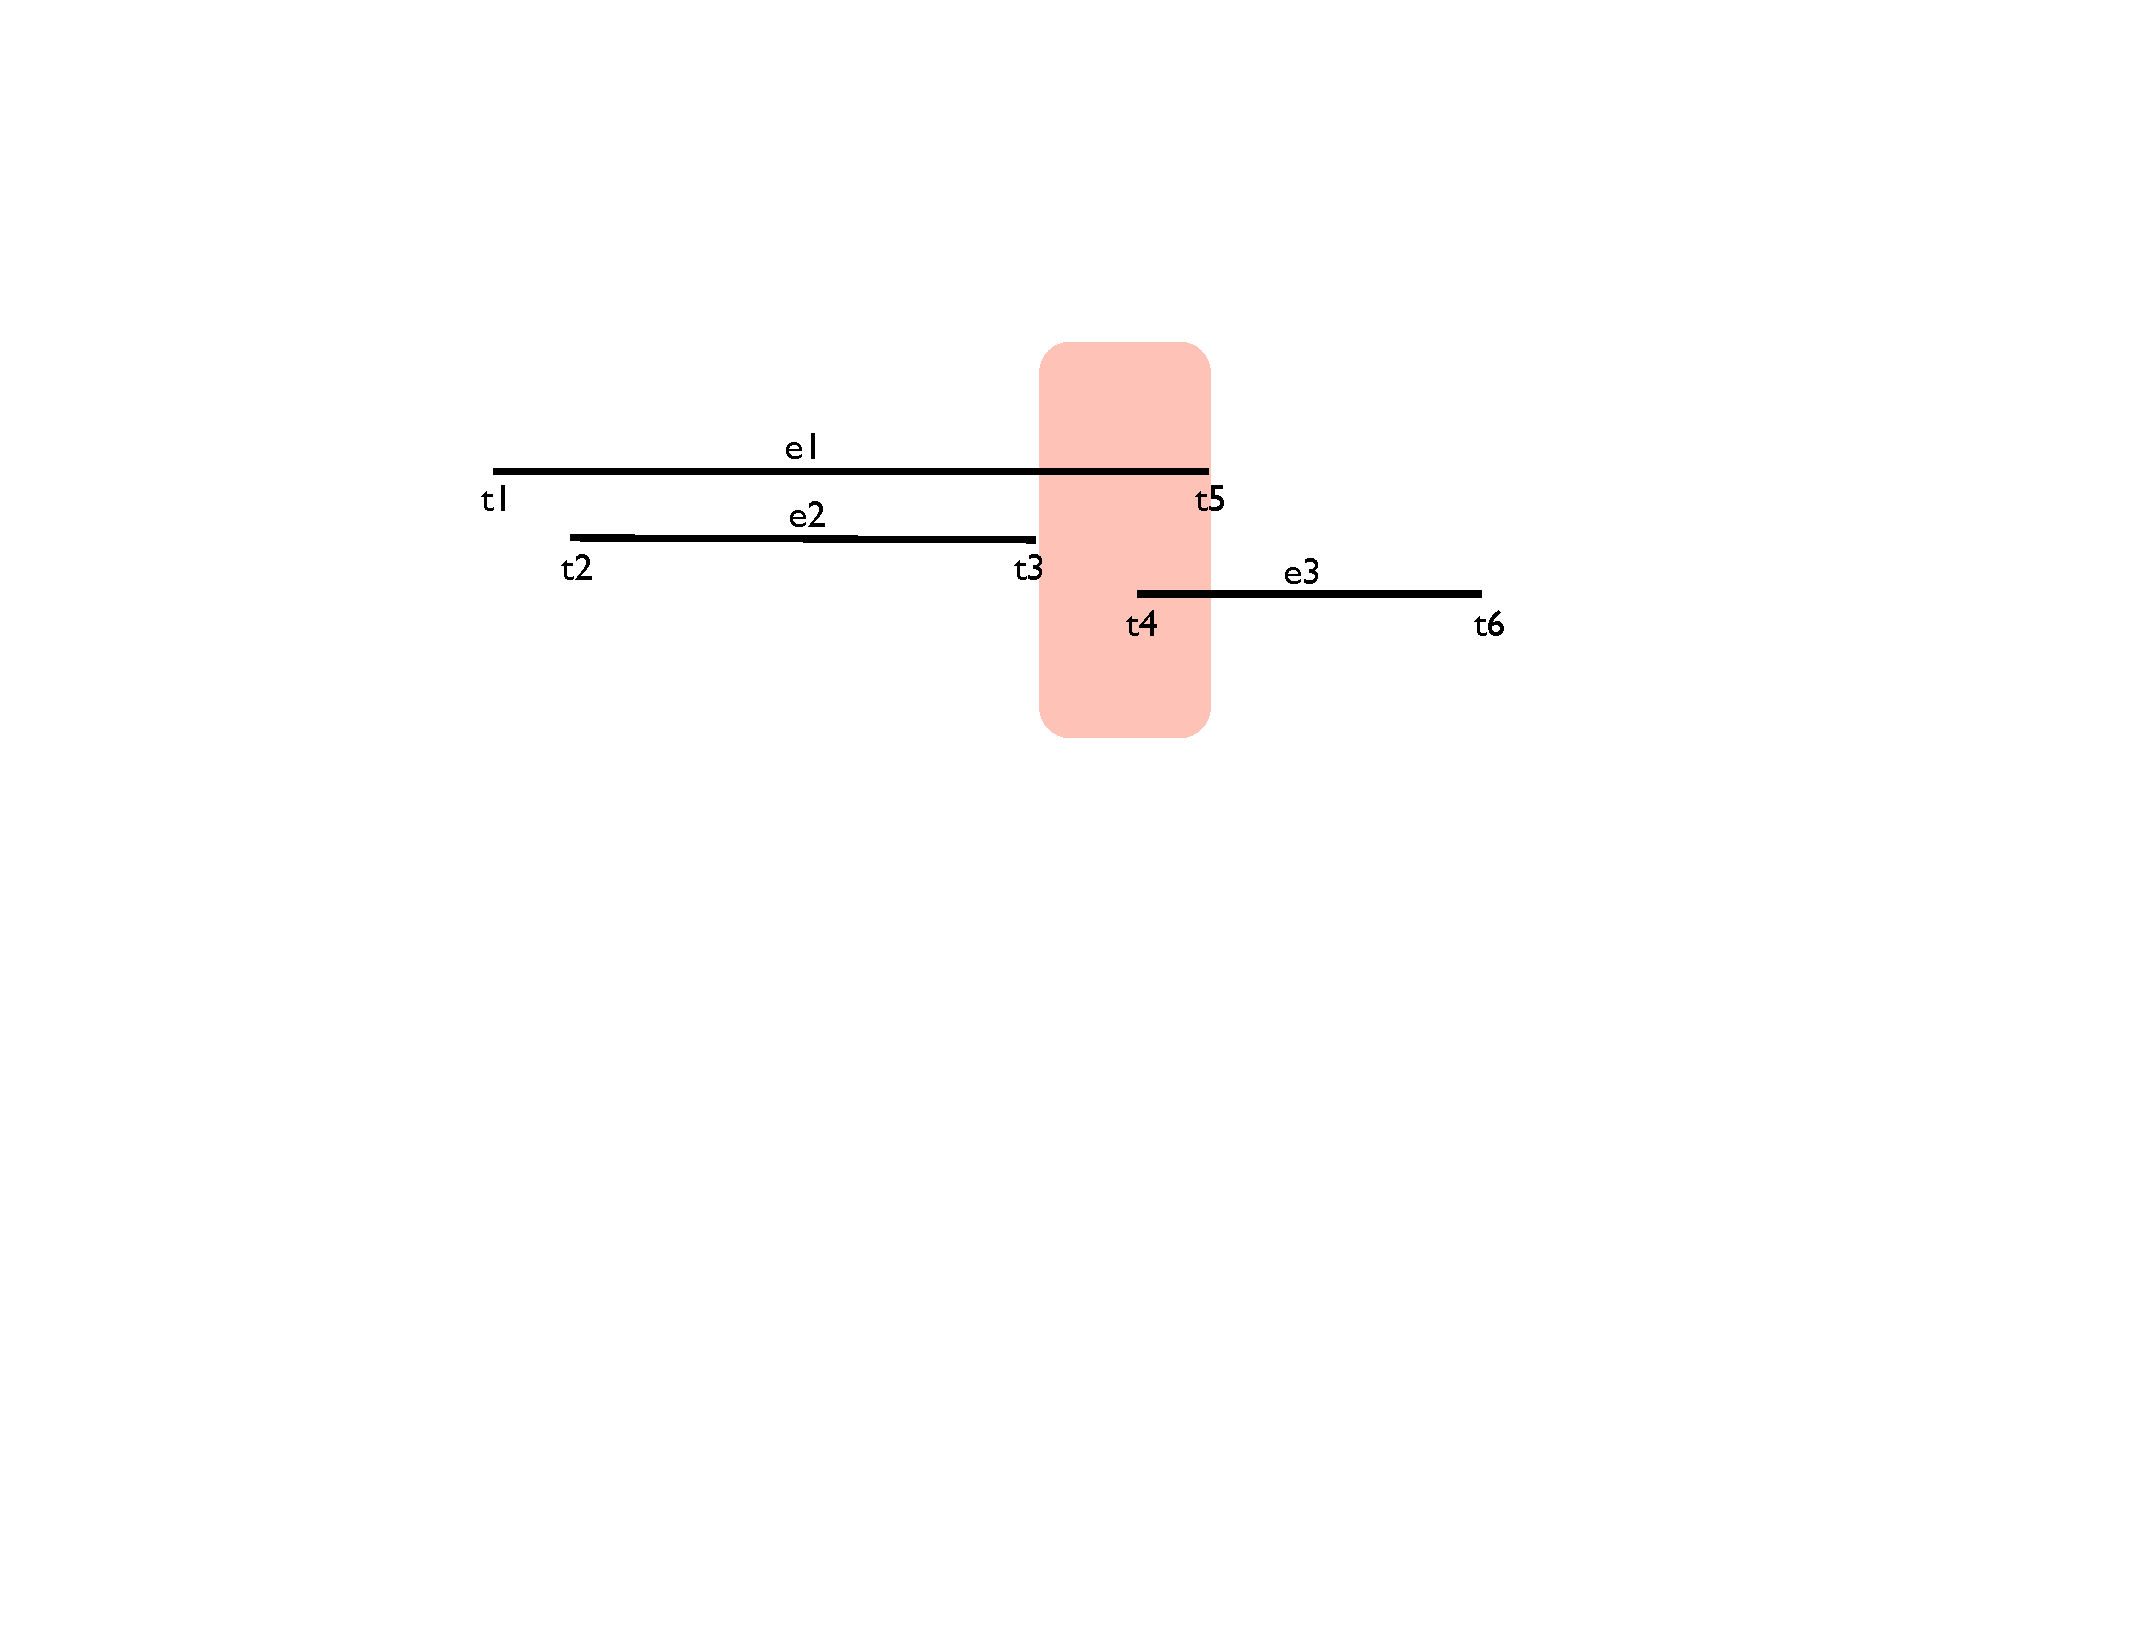
\includegraphics[width=0.6\textwidth]{resources/qp_relaxed.pdf}
		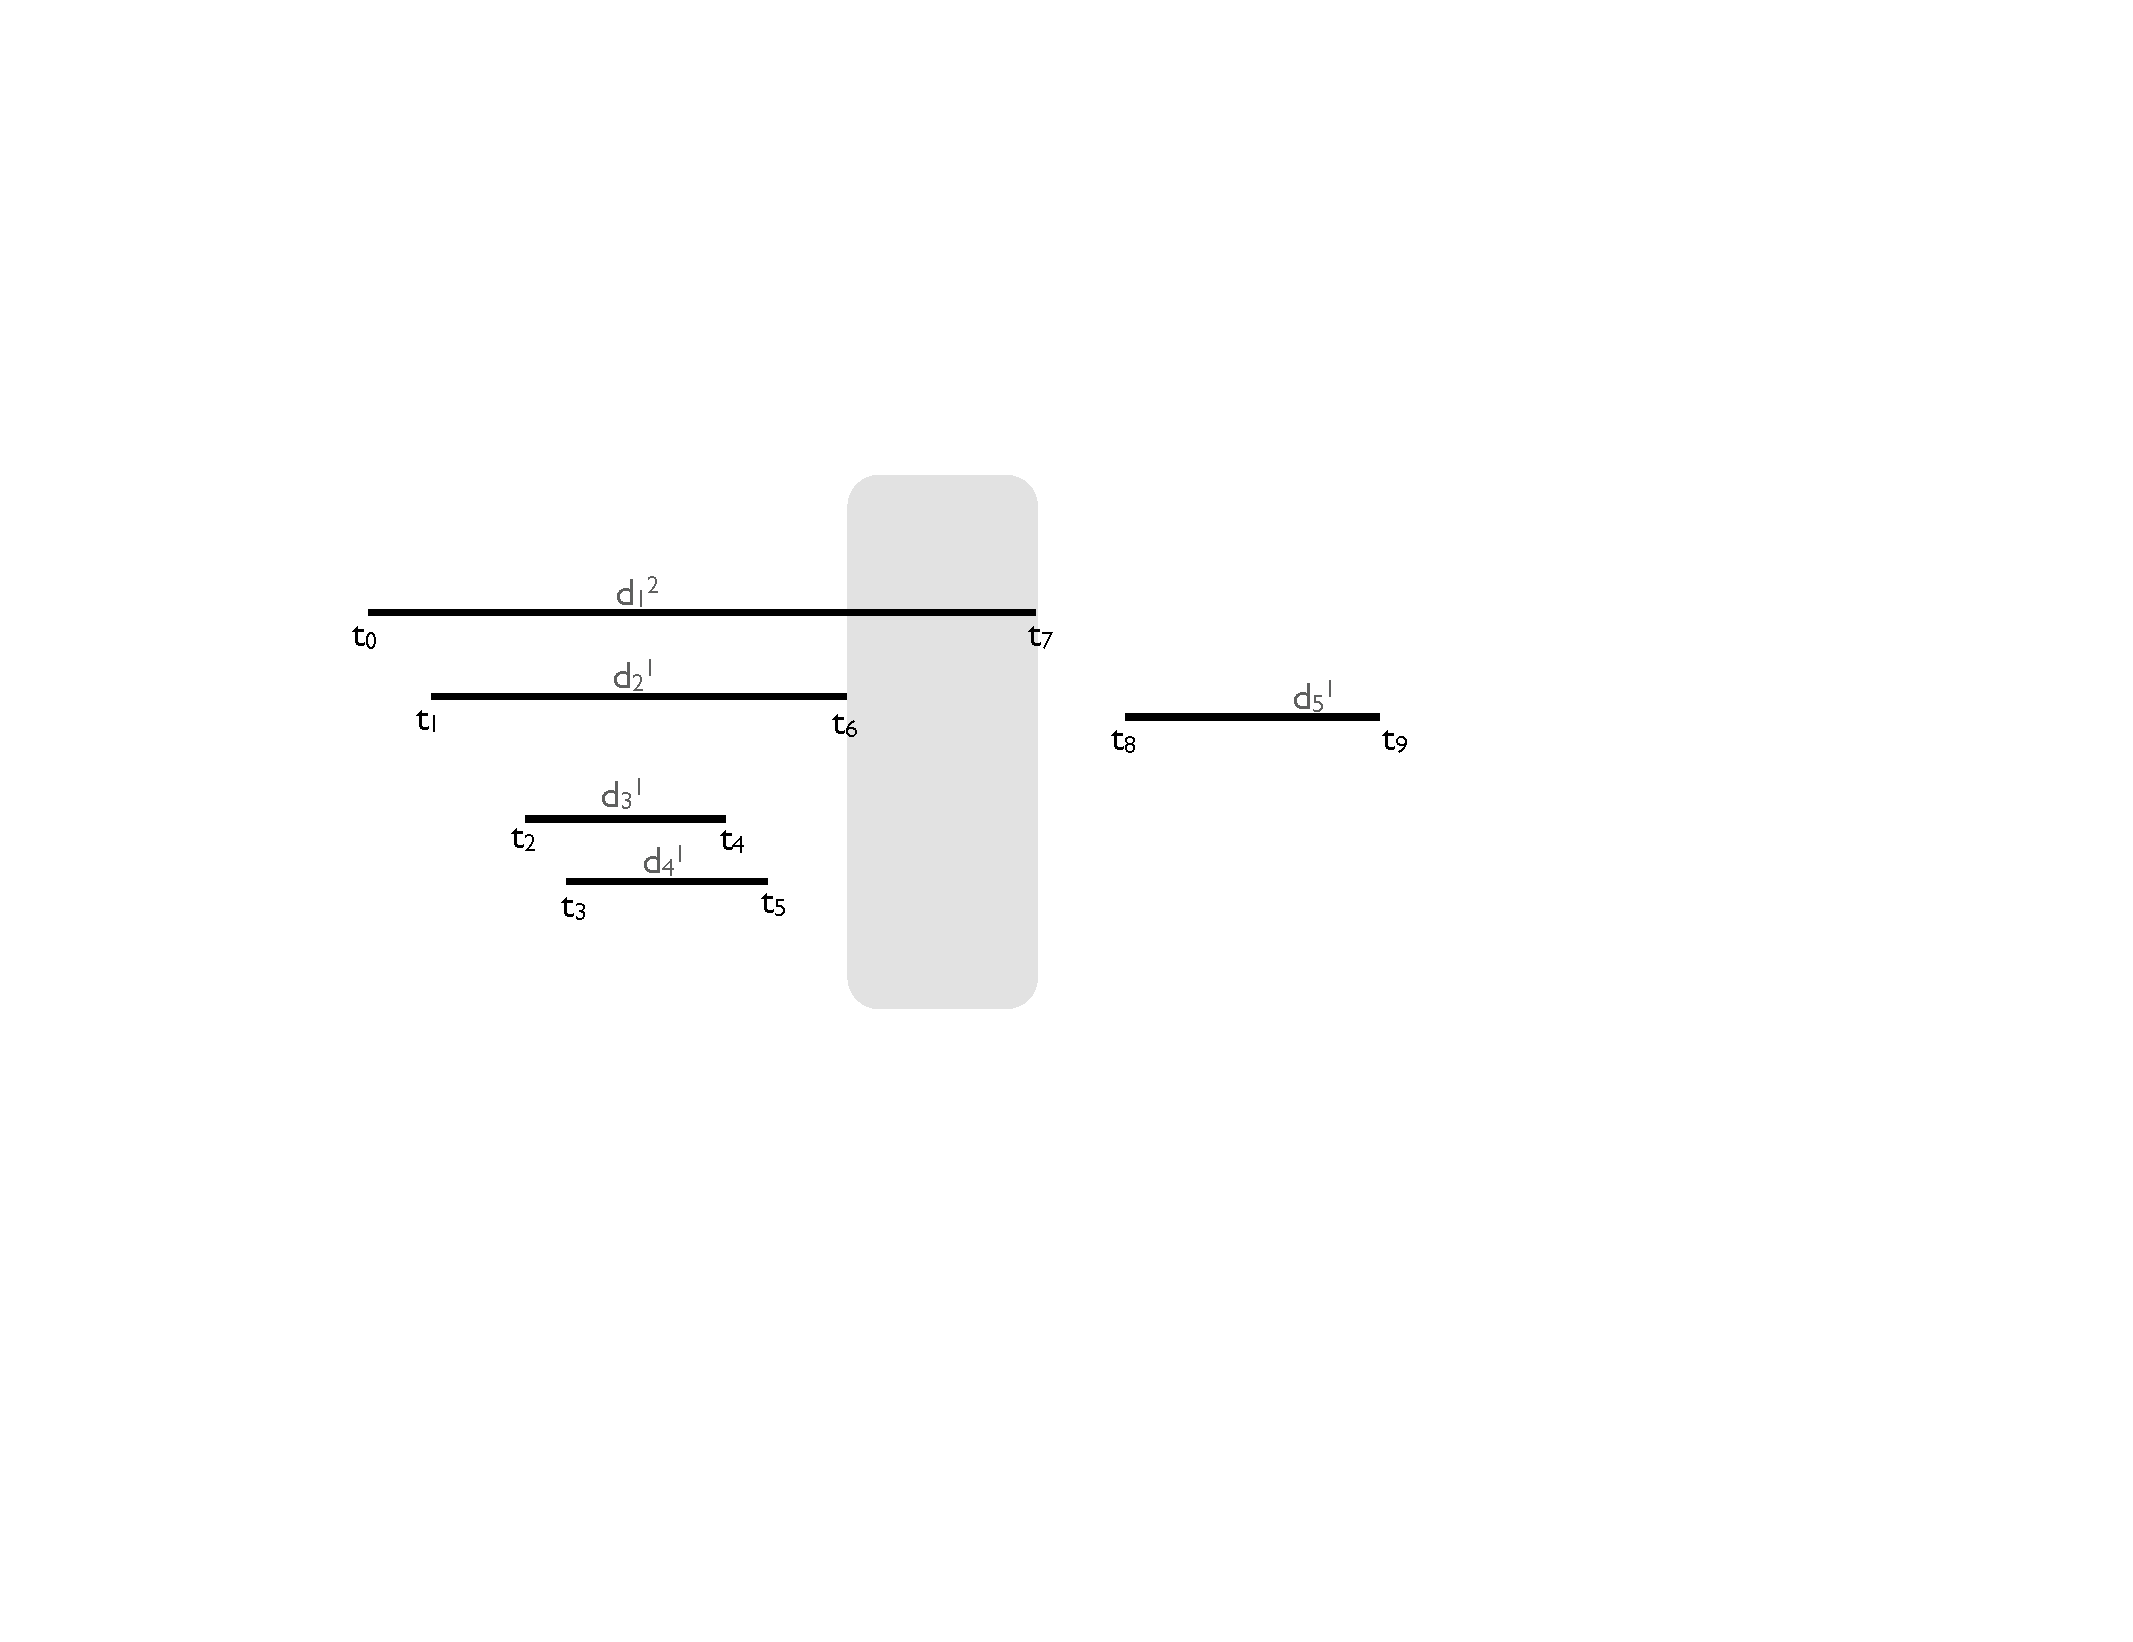
\includegraphics[width=0.8\textwidth]{resources/subsumption.pdf}
	\caption{Subsumption of postings}
	 \label{fig:subsumption}
\end{figure}

A shard is said to exhibit subsumption if it has a pair of postings where one subsumes another. Consider a shard in Figure~\ref{fig:subsumption} with 
five postings where $d_1^2 \sqsupset d_2^1$. 
Now, the queries with $end(d_2^1) \leq begin(Q)\leq end(d_1^2)$ (highlighted region in the figure) will wastefully read $d_2^1$, i.e., $d_2^1$ is processed but does not contribute to the result. Such a scenario, where there are postings like $d_1^2$ which span long intervals and subsume many postings, can arbitrarily degrade performance. Building on this example, if we further introduce $n$ postings which are subsumed by $d_2^1$, they are in turn automatically subsumed by $d_1^2$. Consequently, the number of wasteful reads when the query has a begin time $end(d_2^1) \leq begin(Q)\leq end(d_1^2)$ will be $n+1$.

We can avoid any wasteful reads of postings if we can avoid shards with subsumptions of postings. In other words, we require that postings in a shard satisfy the \emph{staircase property}, defined as follows:  

\begin{definition}[Staircase Property]
\label{def:staircase}
A shard $\sigma$ is said to have the staircase property if $\sigma$ has exactly one posting or  
$$\forall p,q \in \sigma, \,\,\, begin(p) \leq begin(q) \, \Rightarrow \, end(p) \leq end(q) \,\,.$$ 

We let the Boolean predicate $staircase(\sigma)$ denote whether $\sigma$ has the staircase property.
\end{definition}


%figure
\begin{figure}[tb]
	\centering
		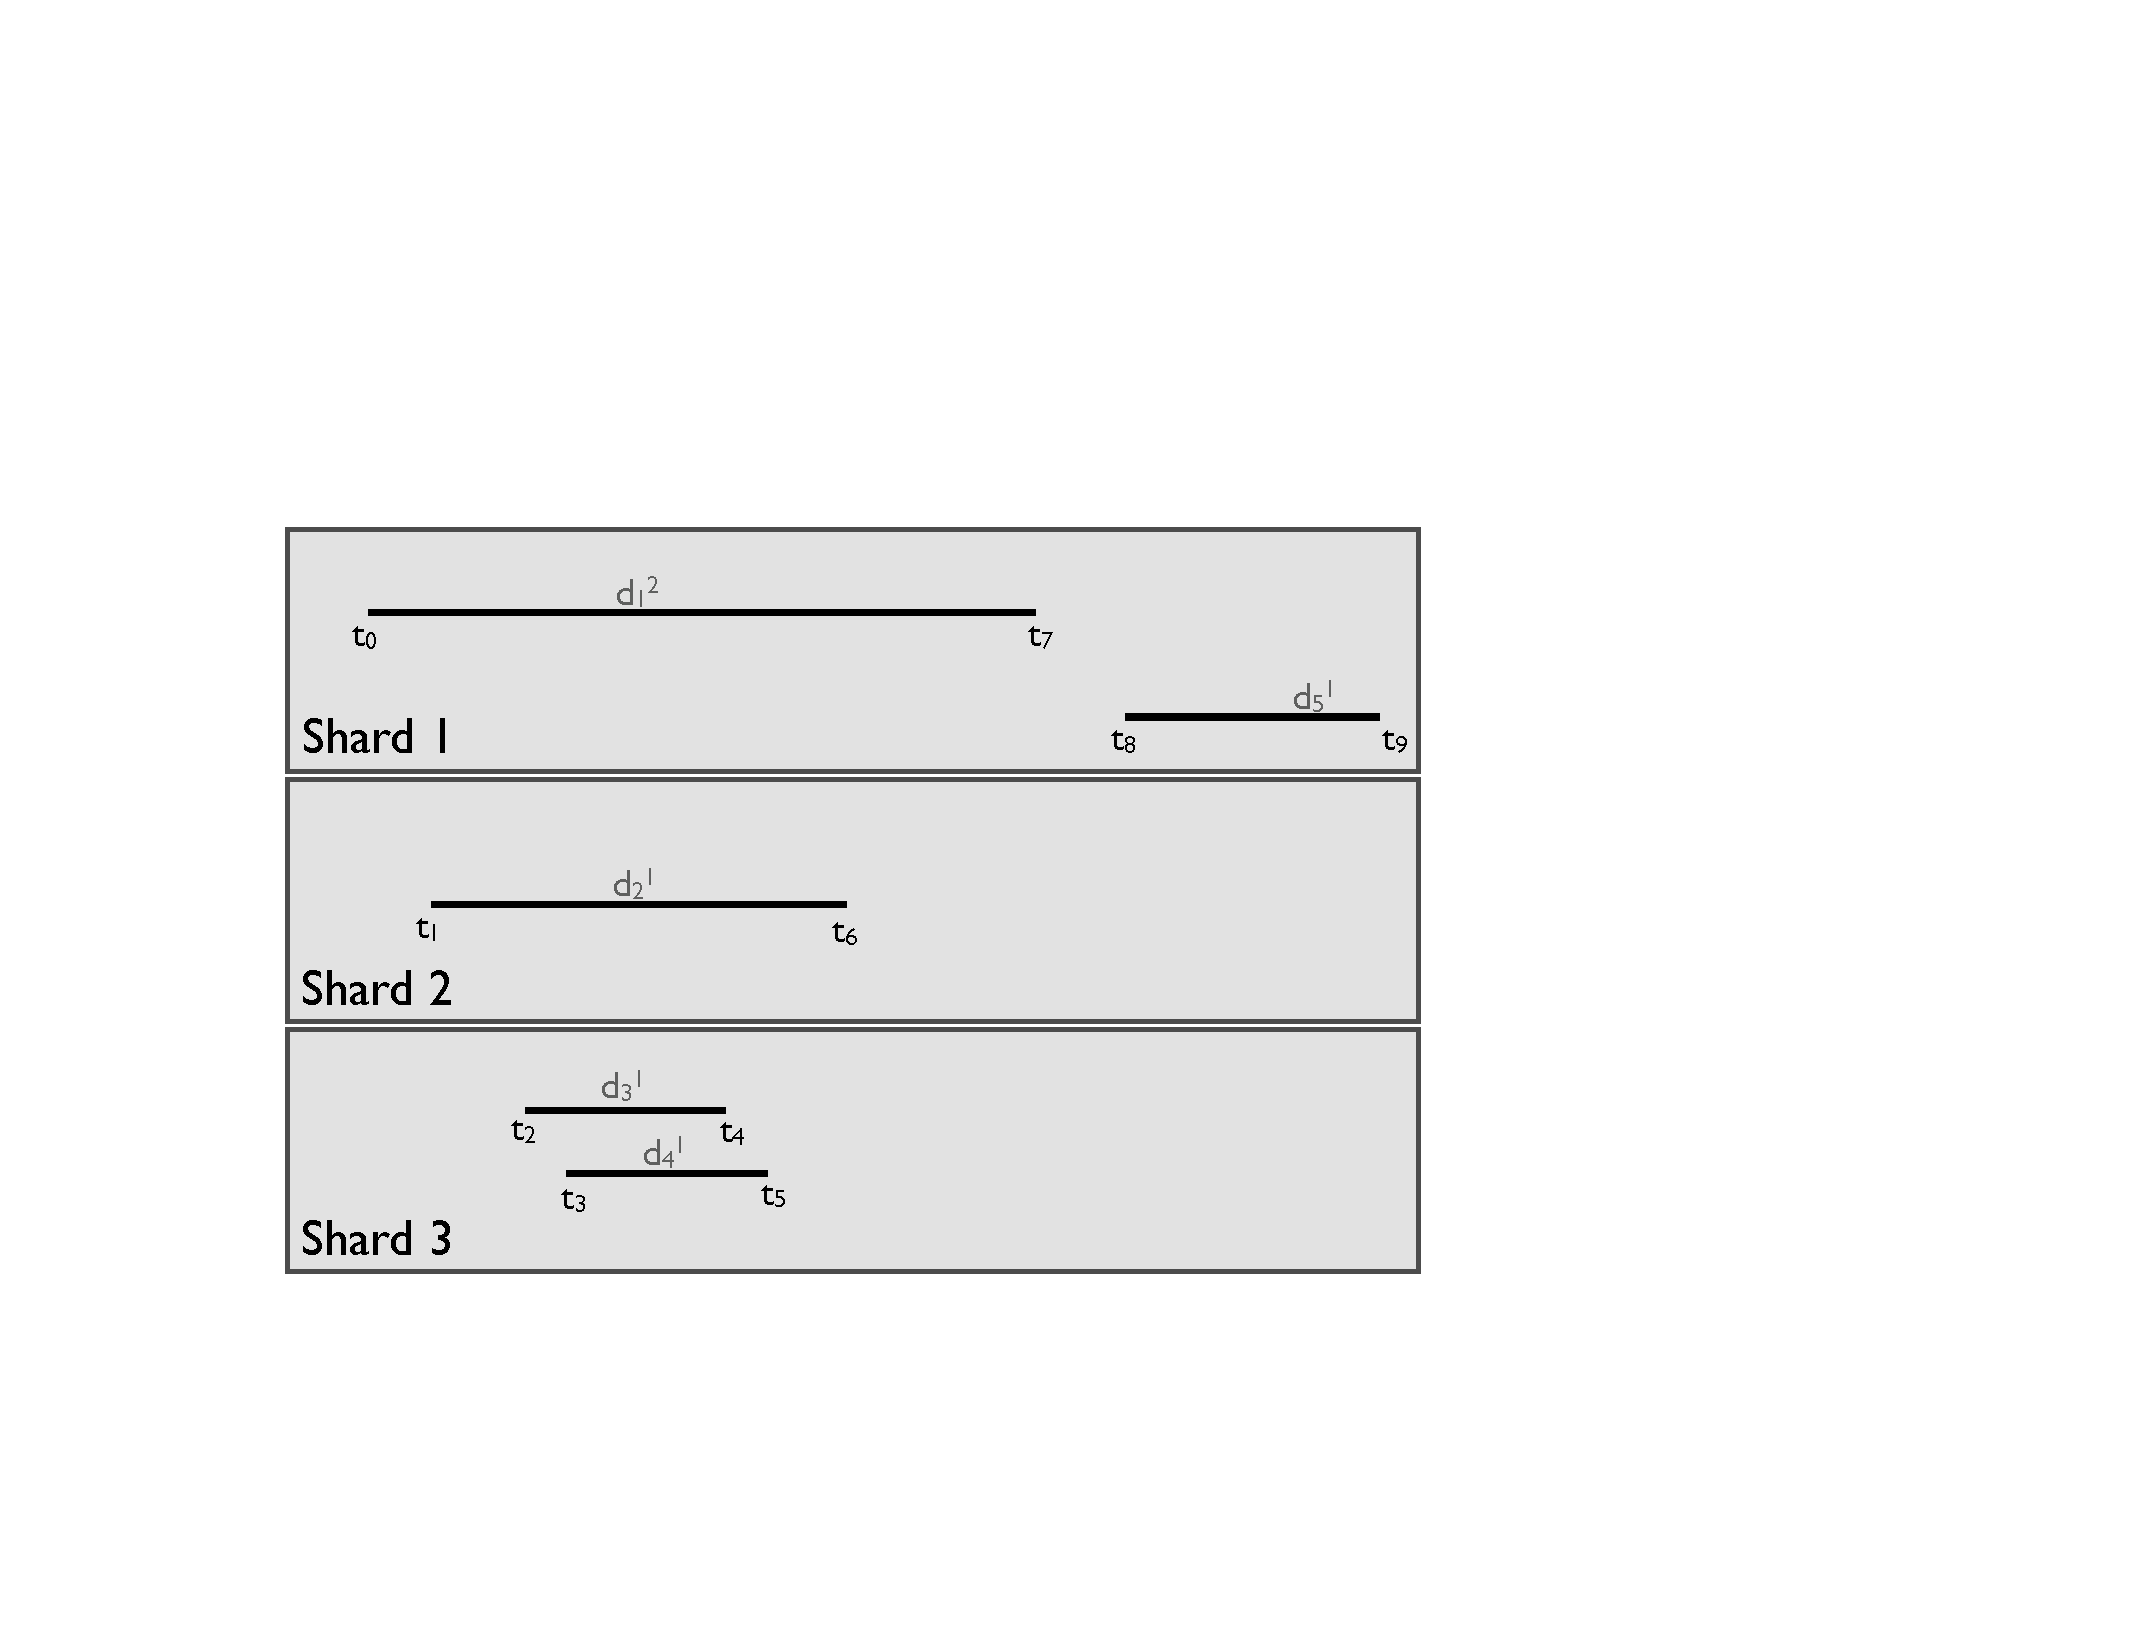
\includegraphics[width=0.6\textwidth]{resources/idealized.pdf}
	\caption{Idealized sharding with staircase property}
	 \label{fig:idealized_sharding}
\end{figure}

Clearly, it may be possible to shard a given posting list in many
different ways so that the staircase property is satisfied. Since query 
processing proceeds by open-skip operations for all shards of a term, 
it is desirable to \emph{minimize} the number of idealized shards. This 
can be cast into an optimization problem with the input being a list of postings $L_v$. The objective is to partition $L_v$ into a feasible index sharding $\mathcal{S}$ so as to minimize the overall number of shards where each shard exhibits the staircase property. Formally, the \emph{idealized-sharding problem} is defined as follows:

\begin{definition}[Idealized-Sharding Problem]
$$
  \argmin{\mathcal{S}}{|\mathcal{S}|}  \quad\mbox{s.t.} \quad \forall \sigma \in \mathcal{S} : staircase(\sigma) \;.
$$ where $\mathcal{S}$ is a feasible index sharding of $L_v$.
	
\end{definition}
%\aanand{Refomulate this opt problem}

\subsection{Optimal Algorithm for Idealized Sharding}
\label{susec:idealized_algo}

 \begin{algorithm}[htb]
   \small
   \begin{algorithmic}[1]
     \STATE  \emph{Input:} $L_v$ sorted in increasing order of begin times
    \STATE $\mathcal{I}_v = \emptyset$ \quad // Idealized sharding
 	
 	\STATE \FOR{$i = 1\,..\,|L_v|$} 
	\STATE // Iterate over all postings in the posting list for $v$
%		\STATE $\sigma_{t} = \emptyset$
        \IF {$\neg \exists \sigma \in \mathcal{I}_v : \sigma.end \, \leq \, end(L_v[i])$} 
        		\STATE create \textbf{new shard} $\sigma_{new}$ \\
			\STATE $\sigma_{new}.end = 0$
                        \STATE $\mathcal{I}_v = \mathcal{I}_v \cup \{\sigma_{new}\}$
        \ENDIF

\STATE $\sigma_{t} =\argmin{\sigma\, \in \,\mathcal{I}_v} (end(L_v[i]) - \sigma.end)$ \\
        
\STATE $\sigma_{t}.end = end(L_v[i])$ // Update the end time of the shard
		\STATE $\sigma_{t} = \sigma_{t}  \cup \{L_v [i]\}$	// Include the current posting into the shard
\STATE
   	\ENDFOR
\STATE
\STATE\emph{Output:} $\mathcal{I}_v$  is the idealized sharding.

   \end{algorithmic}
   \caption{Idealized sharding algorithm}
   \label{chap:sharding:alg:hor_opt}
 \end{algorithm}

We solve the idealized-sharding problem optimally using the greedy  
algorithm described in Algorithm~\ref{chap:sharding:alg:hor_opt}. We let the last posting added to $\sigma$ be denoted by $last(\sigma)$. We additionally let each shard $\sigma$ be associated with an end time $\sigma.end$ representing the end time of $last(\sigma)$, i.e., $\sigma.end = end(last(\sigma))$.

We process all postings of a list $L_{v}$ in increasing begin-time order. In each iteration, we try to add a posting $L_{v}[i]$ to an existing shard if the end time of $L_{v}[i]$ is greater than the end time of the shard, i.e., $end(L_{v}[i]) \geq \sigma.end$. If there are multiple shards to which $L_{v}[i]$ can be assigned, we
 add it to the shard with the minimum gap, i.e., $end(L_{v}[i]) - \sigma.end$. If there are currently no shards to which $L_{v}[i]$ can be added, we start a new shard with $L_{v}[i]$ in it. 

\subsection{Proof of Optimality}
We develop the proof of optimality of Algorithm~\ref{chap:sharding:alg:hor_opt}
by first proving three lemmas about key properties of the
generated shards. Let the shards created by
Algorithm~\ref{chap:sharding:alg:hor_opt} for a list $L_{v}$ be numbered by their
order of creation starting with $\sigma_1$, i.e., $\sigma_1$ was created before $\sigma_2$ and so on.

The first lemma states that the algorithm produces only shards that
have the staircase property.

\begin{lemma}[Staircase Property]
\label{lem:staircase_property}
		When Algorithm~\ref{chap:sharding:alg:hor_opt} terminates, every shard created by the algorithm has the staircase property.
\end{lemma}
\begin{proof}{}
We show this by contradiction. Assume that there is a shard $\sigma$ that does
 not have the staircase property. This means that there is a pair of postings 
 $p$ and $q$ in this shard such that $begin(p)\leq begin(q)$, and $end(p
 ) > end(q)$ or $q \sqsubset p$. Since $begin(p) \leq begin(q)$, $p$ was added to the shard 
 before $q$. But when $p$ was added, the end time of the shard was set to $
 end(p)$ or $\sigma.end = end(p)$. Thus $q$ could not have been be added to the same shard, which contradicts our assumption.
 %\qed
\end{proof}

\begin{lemma}[Descending-End Times]
\label{lem:descending_endtimes}
If Algorithm~\ref{chap:sharding:alg:hor_opt} created a shard $\sigma_i$ before $\sigma_{j}$, i.e. $i > j$, then $\sigma_i.end > \sigma_{j}.end$.
\end{lemma}

\begin{proof}{} We prove this property by induction over increasing number of postings added. 

$\mathbf{i = 1}$: For the first posting $e_1$ the property holds since there are no earlier shards. 

$\mathbf{i \rightarrow i+1}$: Let there be $n$ existing shards $G = \{ \sigma_1 \cdots \sigma_n \}$. Depending on the end time of the $i+1$th posting, i.e., $end(e_{i+1})$ we consider two cases:

If $end(e_{i+1})$ is less than all the existing shard ends  ($end(e_{i+1}) < \sigma_k.end \,\, ,\forall \sigma_k \in G$), then $e_{i+1}$ forms a new shard and the end of the shard is less than all the existing ends. This proves the claim.

Due to the induction hypothesis, the end times of shards are sorted in the descending order i.e., $\sigma_1.end > \sigma_2.end > \cdots > \sigma_n.end$. If $end(e_{i+1})$ is greater than any of the shards, then by definition (line 6), it will have to be added to the shard which minimizes the difference of their end times. It is easy to see that this shard is the earliest shard which can accommodate $e_{i+1}$ since any other shard will either violate the staircase property or have a greater difference. This proves the claim. 
\end{proof}


\begin{lemma}[Temporal Subsumption of Postings]
\label{lemma:subsumption}
For every posting in a shard $\sigma_i$ ($i > 1$) there exists a posting in $\sigma_{i-1}$ which completely subsumes it.
\end{lemma}
\begin{proof}{} When a posting $p$ is added to shard $\sigma_i$ it is the last added posting, i.e., $last(\sigma_i) = p$. Since we process all the postings in begin-time order, all postings which have been placed into shards before have a begin time less than $begin(p)$. And, from the property of descending-end times $end(last(\sigma_{i-1})) > end(last(\sigma_{i}))$. Thus, at this current execution state of the algorithm the posting $last(\sigma_{i-1})$ completely subsumes $p$, i.e., $last(\sigma_{i-1}) \sqsupset last(\sigma_{i}) $.  
\end{proof}


We now introduce the notion of a \emph{stalactite set} of time intervals which is essential for the rest of the proof. 

\begin{definition}[Stalactite Set]
	\label{def:stalactite}
	A stalactite set $\Upsilon$ consists of time intervals such that,
	$$\forall p, q \in \Upsilon, begin(p) \leq begin(q) \Rightarrow end(p) > end (q) .$$
	%\hfill $\Box$
\end{definition}

There may be many such stalactite sets that can be formed using postings from a given posting list, $L_{v}$. Let us denote the stalactite set of maximum cardinality as $\Upsilon_{max}(L_{v})$.

\begin{lemma}[Stalactite property]
	\label{lem:stalactite_property}
			The number of shards created by Algorithm~\ref{chap:sharding:alg:hor_opt} for a list $L_v$ is equal to $|\Upsilon_{max}(L_v)|$.
\end{lemma}

\begin{proof}{} We prove the lemma by contradiction. Assume that the new posting to be added $e_{new}$ is not a part of $|\Upsilon_{max}(L_v)|$. We also assume that its addition creates a new shard $\sigma_{|\Upsilon_{max}(L_v)|+1}$ which is more than the claimed $|\Upsilon_{max}(L_v)|$ shards. Since the postings arrive in begin-time order, $begin(e_{new})$ is greater than any of the previously processed postings. This means that $end(e_{new}) < end(\sigma_{|\Upsilon_{max}|})$ for it to start a new shard $\sigma_{|\Upsilon_{max}|+1}$. Now Lemma~\ref{lemma:subsumption} says that there exists a posting in $\sigma_{|\Upsilon_{max}|}$ which subsumes $e$, making $e$ a part of a larger stalactite set of cardinality $|\Upsilon_{max}|+1$ which is contrary to initial assumption that $\Upsilon_{max}$ is the maximal stalactite set.
\end{proof}

We can now prove the optimality of our algorithm for idealized sharding.
%\newtheorem{theorem}{Theorem}
 \label{hor_opt-thm}
\begin{theorem}
  Algorithm~\ref{chap:sharding:alg:hor_opt} creates an optimal sharding.
\end{theorem}

\begin{proof}{}
	Lemma~\ref{lem:staircase_property} establishes that there are no subsumptions in a shard. Since $\Upsilon_{max}(L_v)$ is the maximum size stalactite set, from Lemma~\ref{lem:staircase_property}, the overall number of shards are lower bounded by $|\Upsilon_{max}(L_v)|$. However, Lemma~\ref{lem:stalactite_property} proves that we exactly obtain $|\Upsilon_{max}(L_v)|$ shards by idealized sharding. This proves that the optimal solution to the idealized sharding of $L_v$ has $|\Upsilon_{max}(L_v)|$ shards thus proving the optimality of Algorithm~\ref{chap:sharding:alg:hor_opt}.
\end{proof}

Further, we show that the algorithm can be implemented efficiently, by
making use of the descending-end times property of the sharding at any stage during the algorithm. Due to this ordering of shard ends the addition step of postings to shards can be efficiently implemented via a binary search over the shard ends.

\section{Cost-Aware Merging of Shards}
\label{chap:sharding:sec:relaxed_part}

Depending on the distribution of valid-time intervals, the idealized
sharding introduced in the previous section might generate a large
number of shards. Each shard requiring one \emph{open-seek} operation, 
involving a random seek.  If the cost of such a random seek is
high and if the distribution of time intervals gives rise to many
idealized shards, query-processing performance can degrade. In such 
cases, it might actually be beneficial to reduce the number of shards 
arising from idealized sharding at the cost of allowing some wasted 
reads.
 
In this section, we present an I/O cost-aware technique to
selectively merge idealized shards allowing for a controlled amount of
wasted reads while reducing the number of random seeks. We introduce a
 model for merging idealized shards which limits sequential wasted reads due to merging of a
set of idealized shards by taking into consideration costs of random
seeks and sequential accesses of the underlying index.

\begin{figure}[tb]
	\centering
		%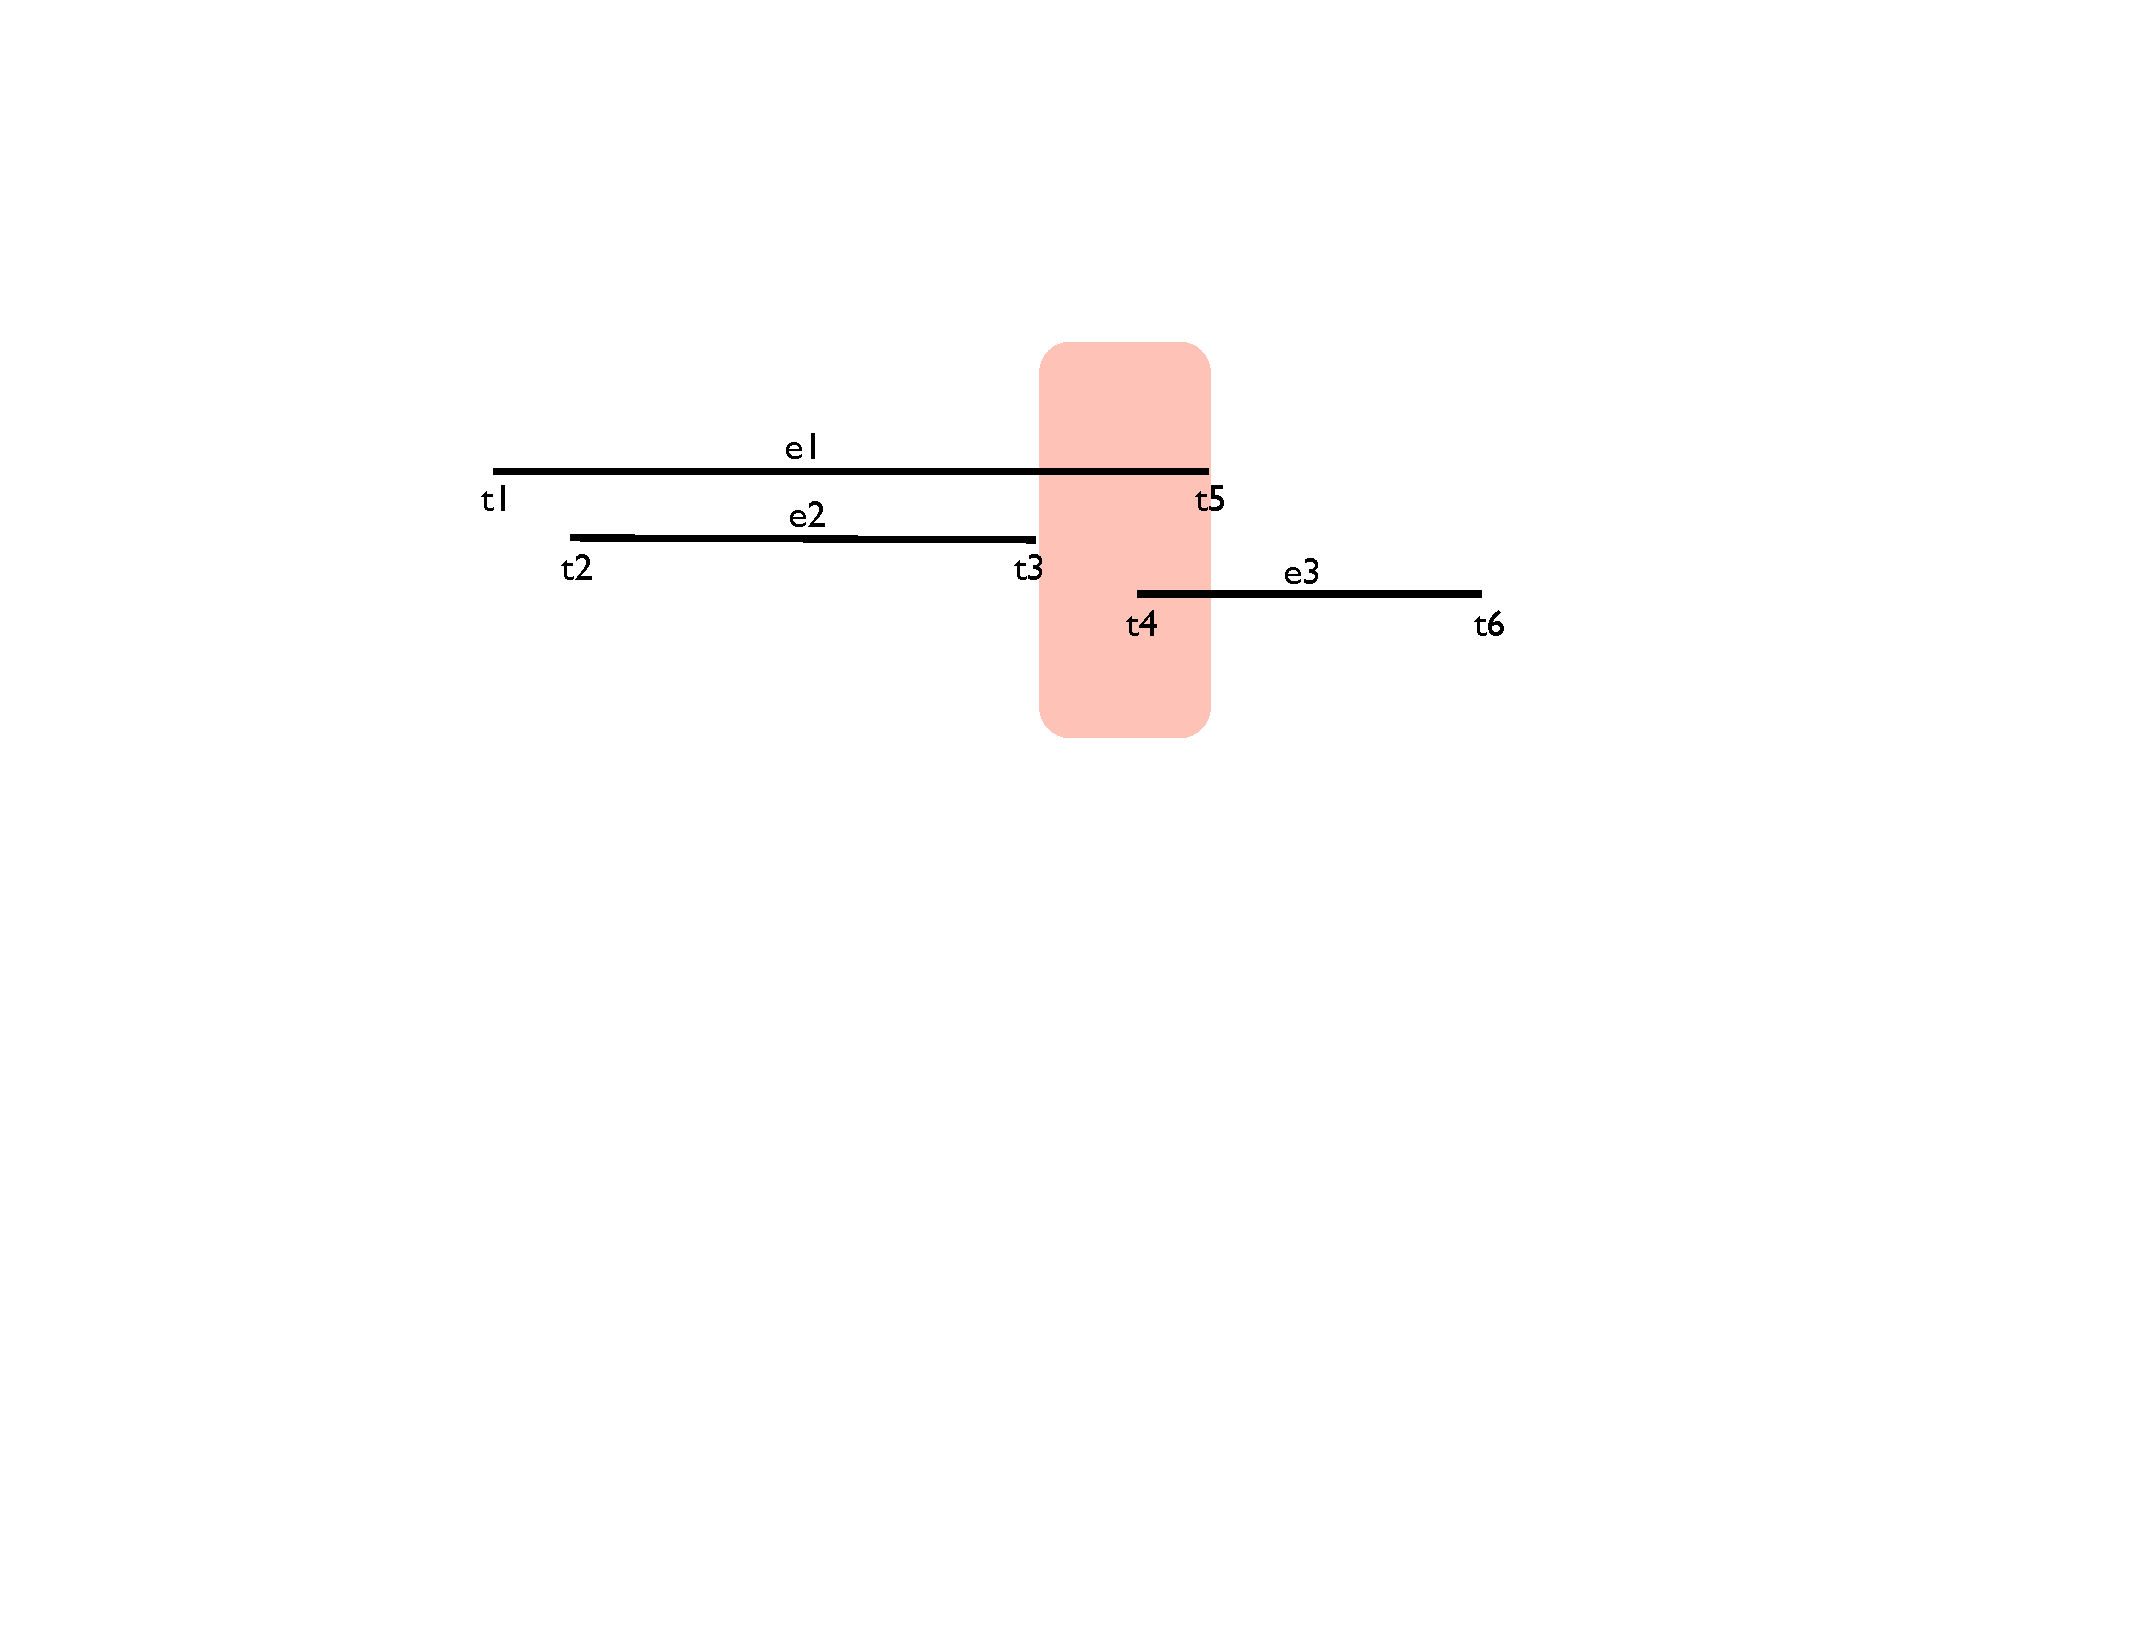
\includegraphics[width=0.6\textwidth]{resources/qp_relaxed.pdf}
		\includegraphics[width=\textwidth]{resources/shard_merging.pdf}
	\caption{Cost-aware shard merging}
	 \label{fig:cas}
\end{figure}
%intuition for the penalty function
\subsection{Model for Shard Merging}

Multiple shards can be merged into a \emph{merged shard} which contains all postings of the input shards and have a begin-time order on the intervals associated with the postings (see Figure~\ref{fig:cas}). We denote a shard created from merging an input set of shards $\mathcal{S}$ as $\mu(\mathcal{S})$. 
In our model we take as input an idealized sharding $\mathcal{I}_v$ of a posting list $L_v$. Our intention is to reduce the overall 
number of shards per posting list by identifying idealized shards which 
can be merged according to our cost model. To this end we propose to 
disjointly partition the input set $\mathcal{I}_v$ into sets or partitions of 
shards $M_v$. Merged shards $\mu(\mathcal{S})$ are then created using 
shards from each partition $\mathcal{S} \in M_v$. The partitioning 
thereby ensures that no two merged shards have postings from the same 
idealized shard. The resulting merged shards, $\mu(\mathcal{S}) \,\,, \,\, \mathcal{S} \in M_v$, thus formed also are a feasible 
index sharding of $L_v$, i.e.,

$$
	\bigcup_{\mathcal{S} \in M_v}{\mu(\mathcal{S})} = L_v.
$$

Merging of shards might result in subsumptions of postings which further leads to wasted reads during query processing. However, not all query time-points lead to wasted reads. For example, in Figure~\ref{fig:subsumption} only queries which have a begin time interval $[t6, t7]$ result in wasted reads. Secondly, an open-seek operation to a merged shard accompanied by a few
sequential wasted reads may be cheaper than two open-seek operations to
idealized shards without any wasted reads. These are two factors which should be taken into considerations in choosing which shards to merge. An accurate estimate of the performance of a shard can be modelled by considering the performance over all query time-points.

\paragraph{Cost Model} We let the cost of a random seek be $C_r$, and that of a sequential read be $C_s$. 
%Since the number of wasted reads incurred is different at different time-points we need a time-based aggregation of performance. 
We allow for a penalty function $\Psi(\mathcal{S})$, over a set of shards $\mathcal{S}$ and require it to be bounded by the parameter $\eta$. To reconcile the costs of random and sequential accesses the parameter $\eta$ is set to $C_r/C_s - 1$. We refer to this bounding of the penalty function as the \emph{threshold criterion}.

$$\Psi(\mathcal{S}) \leq \eta$$

An example of such a penalty function is \emph{expected wasted reads},
which is defined as the number of wasted reads incurred during query
processing, averaged over all possible query time points. 
We define $w(\sigma, t)$ as the set of wasted postings read for a query with a time-point $t$ over a shard $\sigma$. We consider a discrete notion of time and denote the time granularity as $\delta$. If all possible query times lie in the interval $[t_{0}, t_{n}]$ the number of valid query time-points is $\frac{t_{n} - t_{0}}{\delta}$. Formally, 

\begin{definition}[Expected Wasted Reads]
	Given a merged shard $\mu(\mathcal{S})$ and its wasted read distribution $w(\mu(\mathcal{S}), t)$, the expected wasted reads incurred per query time-point is given by
		$$
			\Psi(\mathcal{S}) = \frac{\sum_{t \in [t_{0}, t_{n}]}{\left|w(\mu(\mathcal{S}), t)\right|}}{(t_{n} - t_{0})/ \delta}.
		$$
\end{definition}

Under this penalty function, a set of shards can be merged when the expected wasted sequential reads in the \emph{merged shard} is less than the
overhead incurred in an open-seek operation. If costs of sequential and random accesses are the same, $C_r = C_s$, we obtain $\eta = 0$ which means we resort to idealized sharding. Understandably, with $C_r = C_s$  the cost of accessing a new shard is the same as reading a wasted posting. Thus it is preferable to avoid wasted reads completely in this situation and employing idealized sharding. However, in more practical scenarios $C_r > C_s$.  As an example, if $\eta
= 100$, then the wasted reading of less than 100 postings, that do not
qualify by the temporal constraint, on an average would be more
beneficial than performing a random seek to an additional shard. One can, in principle, use other notions of aggregation measures for $w(\sigma, t)$ and then define the penalty function accordingly. In this work we use expected wasted reads as the penalty function. 


The partitioning of idealized shards can now be formulated as an optimization problem where we have as input a set of idealized shards, the parameter $\eta$, and the penalty function. Like the idealized-sharding problem we would want to minimize the overall number of shards for minimizing the expensive open-skip operations. The \emph{cost-aware shard merging problem} intends to find a partitioning $M_v$ of idealized shards $\mathcal{I}_v$ so as to have minimum number of partitions subject to the threshold criterion on each partition. Formally, 

\begin{definition}[Cost-aware Shard Merging Problem]

$$
\argmin{}{\left|M_v\right|} \quad \mbox{s.t.} \quad \Psi(\mathcal{S})  \leq \eta \,\,: \,\, \forall \mathcal{S} \in M_v.
$$

\label{def:mwr}
\end{definition}


To solve this problem we first look at how we can efficiently determine the penalty of merging a partition or set of idealized shards $\mathcal{I}_v$. 
A partition containing at least two idealized shards will have a non-zero penalty. To compute the overall penalty value of a partition we need to aggregate the wasted read distribution for the combination of shards in the partition over the entire time-period. The combinatorial nature of the problem makes it prohibtive to pre-compute penalty values for all combinations. What we do instead is compute penalty values of pairs of shards and show that the penalty of any partition ($\ge 2$) can be computed efficiently from these pairwise penalties.

Given a partition $S$ of $m$ idealized shards the wasted reads at a query time-point $t$ is $w(\mu(S), t)$. We retain the order in which idealized shards were created, i.e., shards created early have a lower index. We further let $first(\mathcal{S})$ denote the shard which was created first in $\mathcal{S}$. For shards $\sigma_i, \sigma_j, \sigma_k \in S$ and $i < j < k$, it holds 
$$w(\mu({i,k}),t) = w(\mu({j,k}),t).$$ Thus $w(\mu(S), t) = \sum_{\sigma \in \mathcal{S}}{\Psi(\{first(\mathcal{S}),\sigma\})}.$ The penalty $\Psi(\mathcal{S})$ follows from this observation and Definition~\ref{def:mwr}:
$$
\Psi(\mathcal{S}) = \sum_{\sigma \in \mathcal{S}}{\Psi(\{first(\mathcal{S}),\sigma\})}.
$$
 
As an example, the penalty incurred due to merging idealized shards \{7,10,3,12\} would be $\Psi(3,7) + \Psi(3,10) +
\Psi(3,12)$. Computing wasted reads at each time point can be efficiently implemented by interleaving computation of pairwise wasted reads within Algorithm~\ref{chap:sharding:alg:cost_aware_merge}.
 
\subsection{Algorithm for Shard Merging}

\begin{algorithm}[htb!]
   %\small
   \begin{algorithmic}[1]
     \STATE  \emph{Input:} $\mathcal{I}_v$ and ${\Psi(\sigma_{i},\sigma_{j})}$ 
     \STATE $M_v = \emptyset$ \quad // Merged shards
 	
	\STATE \FOR{$i = 1\,..\,|\mathcal{I}_v|$} 
			\STATE Let $\sigma_i \in \mathcal{I}_v \setminus  M_v$ be next shard in order
			\STATE \textbf{create} new shard $r_i$
			\STATE $r_i = r_i \cup \{\sigma_i\} $			
			\STATE $capacity \,=\, \eta$
			\STATE
			\STATE // Ascending choice phase \\
			\FOR{$j = i+1\,..\,|\mathcal{I}_v|$}
				\IF{$(\Psi(\sigma_i,\sigma_j) \leq capacity)\,\,  \wedge \,\,(\sigma_j \notin M_v$)}
					\STATE $capacity \,\, = capacity - \,\, \Psi(\sigma_i,\sigma_j)$
					\STATE $r_i = r_i \cup \{\sigma_j\}$
				 \ELSE \IF{$(\sigma_j \notin M_v) \,\, \wedge \,\,(\sigma_j \notin r_i)$}
					\STATE \textbf{break}
					\ENDIF
				\ENDIF
			\ENDFOR
			\STATE
			\STATE // Smallest size first
			\WHILE {$capacity > 0$}
				    \STATE $\sigma_{min} = \argmin{g \in \mathcal{I}_v \setminus M_v}{\{\Psi(\sigma_i, g)\}}$
					\STATE $capacity \,\, =  capacity - \,\,\Psi(\sigma_i,\sigma_{min})$
					\STATE $r_i = r_i \cup \{\sigma_{min}\}$
			\ENDWHILE
			
			\STATE {$M_v = M_v \cup r_i$}
		\ENDFOR
\STATE
\STATE\emph{Output:} $M_v$ is the set of merged shards.

   \end{algorithmic}
   \caption{Cost-Aware Shard Merging}
   \label{chap:sharding:alg:cost_aware_merge}
 \end{algorithm}


We present a heuristic algorithm which is shown to perform well in
practice in our experimental evaluation. As inputs we expect the set
of the idealized shards and $\eta$. We retain the order
in which idealized shards were created, i.e., earlier created shards
have a lower index.

The pseudo code for merging the idealized shards is presented in
Algorithm~\ref{chap:sharding:alg:cost_aware_merge}. Every iteration employs a two
stage greedy process. The first stage is an \emph{ascending choice
  phase} in which it chooses all the unmerged/available idealized
shards in ascending order of their index until the threshold
constraint is violated (lines 11 to 20).

The second stage is a greedy phase (lines 23 to 27) where the
remaining capacity is greedily chosen with smallest unmerged shard
first (as in the standard greedy approach to the knapsack problem).

\section{Index Maintenance}
\label{chap:sharding:sec:maintenance}
%The indexing techniques discussed so far assumes a static document collection but in practice archives grow dynamically. 
So far, we have assumed a static document collection. These indexing techniques are fine for collections that change infrequently or never. In such cases, occasionally rebuilding indexes is a viable solution in practice. However, for web archives, which grow frequently and dynamically, the index needs to be updated frequently. New terms are added to the index and shards for existing terms are modified. In this section we describe index-maintenance strategies to deal with dynamic updates. We first discuss our assumptions about the nature of the updates in an archive setting and the factors relevant for indexing.

%The indexing techniques described assumed a static text collection.

Updates in web archives are a result of periodic crawls. An update might result in either (i) new \emph{unseen} document, or (ii) report  modifications to an already existing document. Recollect that in Section~\ref{chap:sharding:sec:model} we established the document model where each document is a sequence of versions. Modifications to an existing document, either addition or deletion of content, results in the creation of a new version in the document version sequence. If a new document is reported, a new sequence is started for the document with the reported version being the first. Importantly, existing versions are never removed. This means that the index steadily grows over time with the older collection indexed by the archive index being a subset of the current collection. We assume that deletions in the past are rare and in our current system arbitrary deletions in the past are not supported.

Each version is associated with a valid-time interval. Every update results in a change in the valid-time interval of the \emph{ current version} of each document. Consider the state of the archive at time $t_{now}$ when it was updated. If the update reports no change in the state of a document version $d_i^4$ (document $d$ at its fourth version) the end of the valid-time of $d_i^4$ is updated to $t_{now}$. On the contrary if a new version for $d$ would have been reported, the end time of $d_i^4$ would have been \emph{finalized} to $t_{now}$ (never to be modified again). Additionally, the fifth version $d_i^5$ would have been started with a begin time as $t_{now}$. An accurate estimate of the valid-time intervals of the versions are determined when they are finalized, and hence they are sent to the indexing pipeline in the order of their end times. 

With these assumptions in mind we distinguish between \textit{active versions}, as the
most recent and still current document versions, and \textit{archive versions}, as the document versions already superseded by a more
recent version of the same document. The active version of a document turns into an archive version when the document is re-crawled and either a new active version is found or the document was removed from the Web. In both cases, the end time of the old version is set to the current time.

During indexing we organize postings for active versions into an \emph{active index} and the archived versions are indexed in an \emph{archive index}. The active index is implemented as an incrementally updatable inverted index~\cite{Buttcher:2008fk,Lester:2008qf}. Depending on the fraction of time-travel queries among all queries posed to the system, posting lists in the active index can be organized to efficiently support queries on active versions or time-travel queries. For the former, postings may be ordered by their document identifier to allow for more efficient query processing, possibly together with additional
structures~\cite{DBLP:conf/cikm/BroderCHSZ03,DBLP:conf/sigir/DingS11,DBLP:journals/tois/MoffatZ96,DBLP:conf/sigir/StrohmanC07}. For
the latter, postings may be ordered by the begin boundary of
their valid-time interval to support efficient filtering of recent
document versions. 

The archive index on the other hand is implemented as a sharded index and is our primary focus. Finally, from the indexing point of view it is preferable to have an updating scheme which appends newly created postings at the end of the posting list. The major benefit of an append operation is that the indexes built for the older indexes can be used as partial solutions to build an up-to-date archive index efficiently thus avoiding recomputation. Recomputation of shards with a non-append based technique (say cost-aware shard merging) is expensive because it involves processing the entire input (existing data along with the new updates) thus limiting its applicability to an update aware indexing system. 

To this end, we develop \emph{incremental sharding} which
\begin{itemize}
	\item is competitive in query processing by trading-off, like shard merging, wasted reads for random-accesses, 

	\item takes into account the end-time order of arrival of input, and	
	\item can be maintained easily because it can be incrementally computed and results in append-only operations to shards.
\end{itemize}

% Incremental Sharding
\section{Incremental Sharding}
\label{chap:sharding:sec:inc_sharding}

Incremental sharding takes into account the relative costs of random and sequential accesses by a more restrictive bound on the number of subsumptions for a given shard. It bounds the absolute number of subsumptions for a given shards. This is opposed to shard merging where the number of subsumptions per shard is on an average limited to a system-wide parameter. A bound on the number of subsumptions per shard translates to bounding the number of sequential wasted reads. We term this restriction as the \emph{bounded subsumption} property. A shard is said to exhibit a bounded subsumption property if a posting in that shard does not subsume more than $\eta$ postings, where $\eta$ is a system-wide constant (same as in sharding merging). Formally,

\begin{figure}[tb]
	\centering
		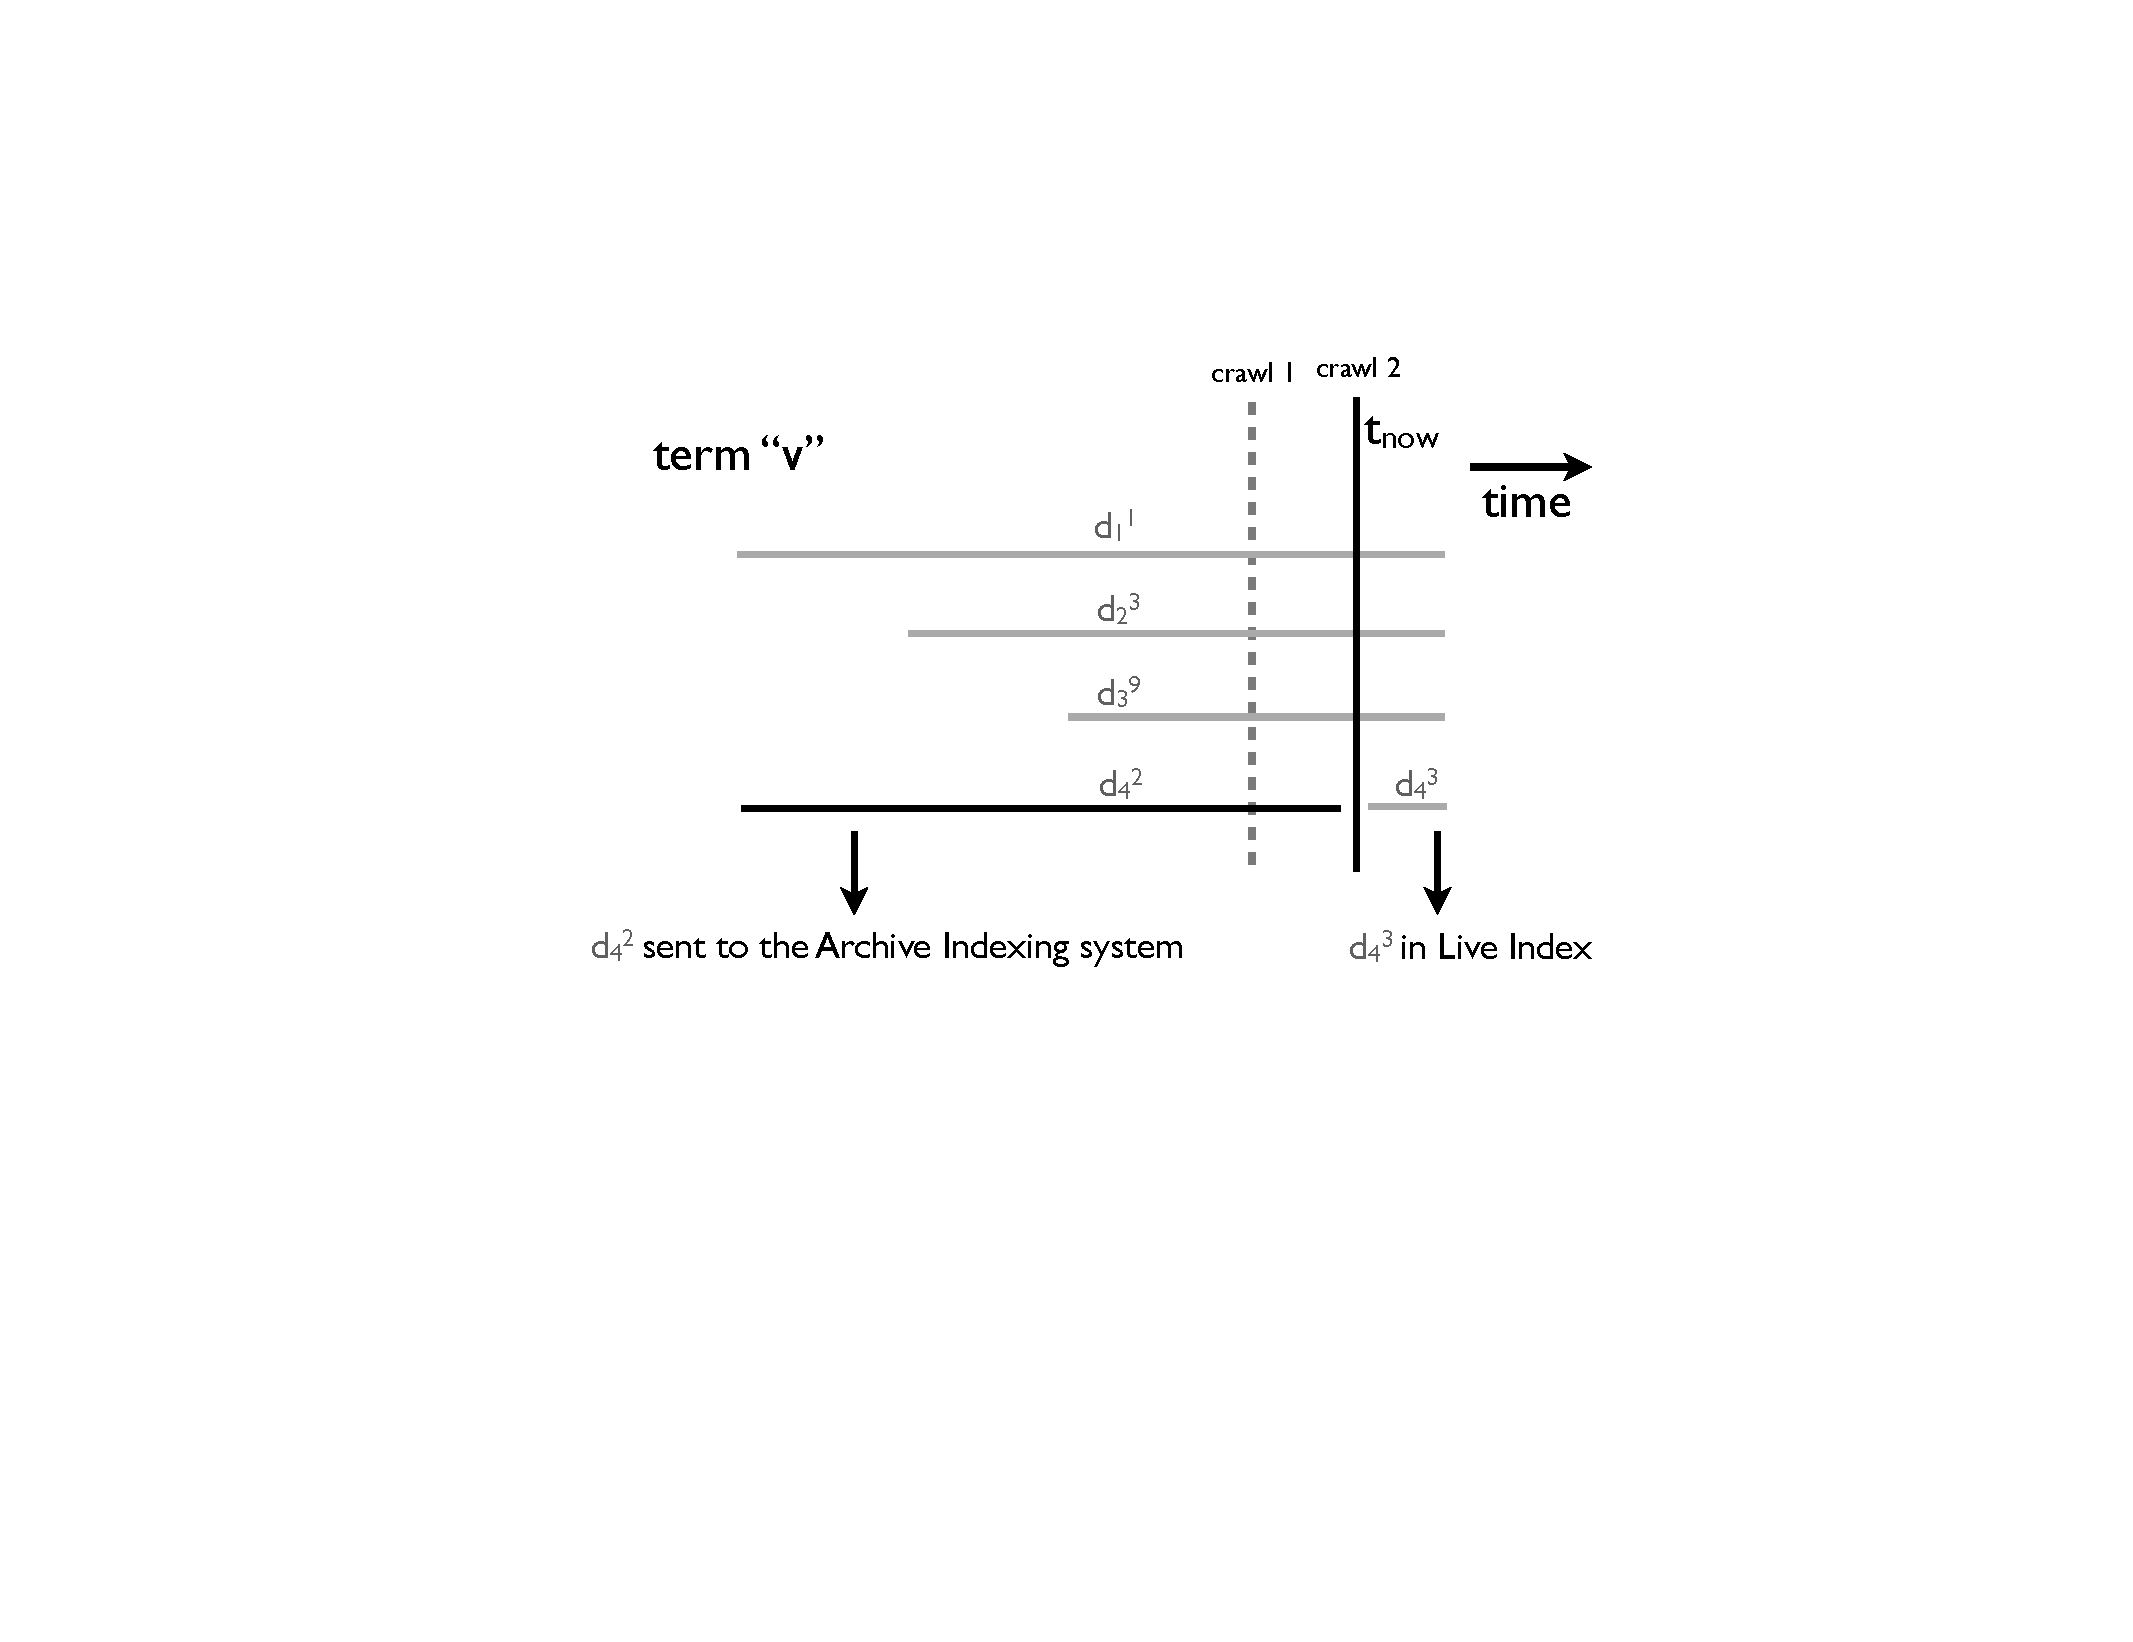
\includegraphics[width=0.8\textwidth]{resources/sliding_wind_grayscale.pdf}
	\caption{End time order of finalizing versions}
	 \label{fig:finalizing_versions}
\end{figure}

\begin{definition}[Bounded Subsumption]
A shard $\sigma$ is said to satisfy the bounded subsumption property with threshold $\eta$ if each posting $p_i \in \sigma$ does not subsume more than $\eta $ postings:
$$ \forall p_i \in \sigma: \vert \,\{ \, p_j \in \sigma \, \mid \, p_j \neq p_i \,\, \wedge \,\, p_i \sqsupset p_j \} \,\vert \,\leq \, \eta  \,\,.
$$

We let the Boolean predicate $bounded(\sigma, \eta)$ denote whether the shard $\sigma$ has the bounded-subsumption property with a threhold $\eta$.
%We say that the boolean predicate $bounded(\sigma, \eta)$ evaluates to true if $\sigma$ satisfies the bounded subsumption propert with threshold $\eta$.
\end{definition}

The problem of minimizing the number of random accesses with a limited number of wasted sequential accesses can be redefined in terms of minimizing the overall number of shards such that each shard exhibits the bounded subsumption. Formally,

\begin{definition} [Incremental Sharding Problem]
Given a set of postings $L_v$ for a term $v$, partition $L_v$ into a feasible index sharding $\mathcal{S} = \{\sigma_1, \ldots, \sigma_{m}\},$ 


$$
  \argmin{\mathcal{S}}{|\mathcal{S}|}  \quad\mbox{s.t.} \quad \forall \sigma \in \mathcal{S} : bounded(\sigma, \eta) \;.
$$

\end{definition}

Before attempting to solve the above problem let us revisit the properties in an archive indexing setting. Firstly, the archive setting is very specific in terms of arrival of the input sequence, i.e., in the order of arrival of new versions to the archive index. Whenever the end time of an existing version is determined, it is sent to the archive indexing system (see Figure~\ref{fig:finalizing_versions}). Since versions are generated in end-time order, the input intervals also follow the same order. 

Secondly, we do not deal with deletions of versions since a deletion of a document results in a posting in the archive index for that document, and existing versions are never removed. 

Finally, we would want to avoid recomputation of shards by only allowing appends to the materialized shards. Apart from avoiding recomputation ensuring an append-only operation also avoids expensive decompression and compression cycles. While merging two posting lists by employing recomputation, entire posting lists are decompressed and re-ordered (according to posting-begin times) to form usable input for the sharding algorithm. After recomputation, the new set of shards are compressed back again for storage. The most popular compression algorithms used in posting list compression are based on gap-encoding schemes which are local schemes and hence append friendly. Hence, rather than optimally solving the problem, we look for an approach which is based on an append-only operation to the existing shards and exploits the end-time order of input arrival. In the following section, we introduce the \emph{incremental sharding} algorithm which apart from being incremental also has an approximation guarantee. 

 \begin{algorithm}[htb!]
   %\small
   \begin{algorithmic}[1]
     \STATE  \emph{Input:} (i)$\eta$, (ii)$L_v$ sorted in increasing order of end times
     \STATE $\mathcal{S} = \emptyset$ \quad // Incremental sharding
 		
	\STATE \FOR{$i = 1\,..\,|L_v|$} 
	\STATE //Creates new shard
        \IF {$\neg \exists S \in \mathcal{S} : S.begin \, \leq \, begin(L_v[i])$} 
        		\STATE create \textbf{new shard} $\sigma_{new}$ and $buf(\sigma_{new})$ \\
			%\STATE $g_{new}.begin = begin(L_v[i])$ 
			%\IF {$\eta > 0$} 
				\STATE $\sigma_{new}.begin = 0$
			%\ENDIF
			
			\STATE \textbf{add} $L_v[i]$ to $buf(\sigma_{new})$  
                     \STATE $S = \mathcal{S} \cup \{\sigma_{new}\}$
        \ENDIF

	\STATE 

			\STATE //Find the best candidate shard for assignment
			\STATE $\sigma_{cand} = \{ \sigma_i \,\,|\,\, \sigma_i \in \mathcal{S} \,\, \wedge  \,\,\sigma_i.begin \leq begin(L_v[i])\}$
			\STATE $\sigma_{t} =\argmin{g\, \in \,\sigma_{cand}} (begin(L_v[i]) - g.begin)$ 

		\STATE
		\STATE //Update buffers and begin times of shards
		\IF { $\sigma_t \neq \sigma_{new}$}
			\STATE \textbf{insert} $L_v[i]$ into $buf(\sigma_{t})$ in begin-time order			 
		\ENDIF
		\IF {$|buf(\sigma_{t})| = \eta+1$}
			\STATE  //first element in the buffer finalized
			\STATE $\sigma_{t}$ = $\sigma_{t} \,\, \cup$  $removefirst(buf(\sigma_{t}))$
			\STATE  $\sigma_{t}.begin$ = $begin(first (buf(\sigma_t)))$
		\ENDIF        
   	\ENDFOR 
	\STATE
	\STATE //Finally append the buffer postings to the shards
	\FOR {$S \in \mathcal{S}$}
		\STATE	$S \,\,= \,\, S \,\cup buf(S)$
	\ENDFOR
\STATE
\STATE\emph{Output:} $\mathcal{S}$  is the incremental sharding.

   \end{algorithmic}
   \caption{Incremental sharding algorithm}
   \label{chap:sharding:alg:rs-inc}
 \end{algorithm}


\subsection{Incremental Sharding Algorithm}

We present the \emph{incremental sharding algorithm} which is an update aware incremental algorithm with a factor $(2  -  \frac{2}{\eta+2})$ approximation guarantee (see Algorithm~\ref{chap:sharding:alg:rs-inc}). Apart from having the natural benefit of being an append-only algorithm, it also exploits the end-time arrival order of the postings %(c.fSection~\ref{fig:finalizing_versions}) 
by processing the postings in that order thus avoiding expensive sort operations on the input. 

\begin{figure}[tb]
	\centering
		%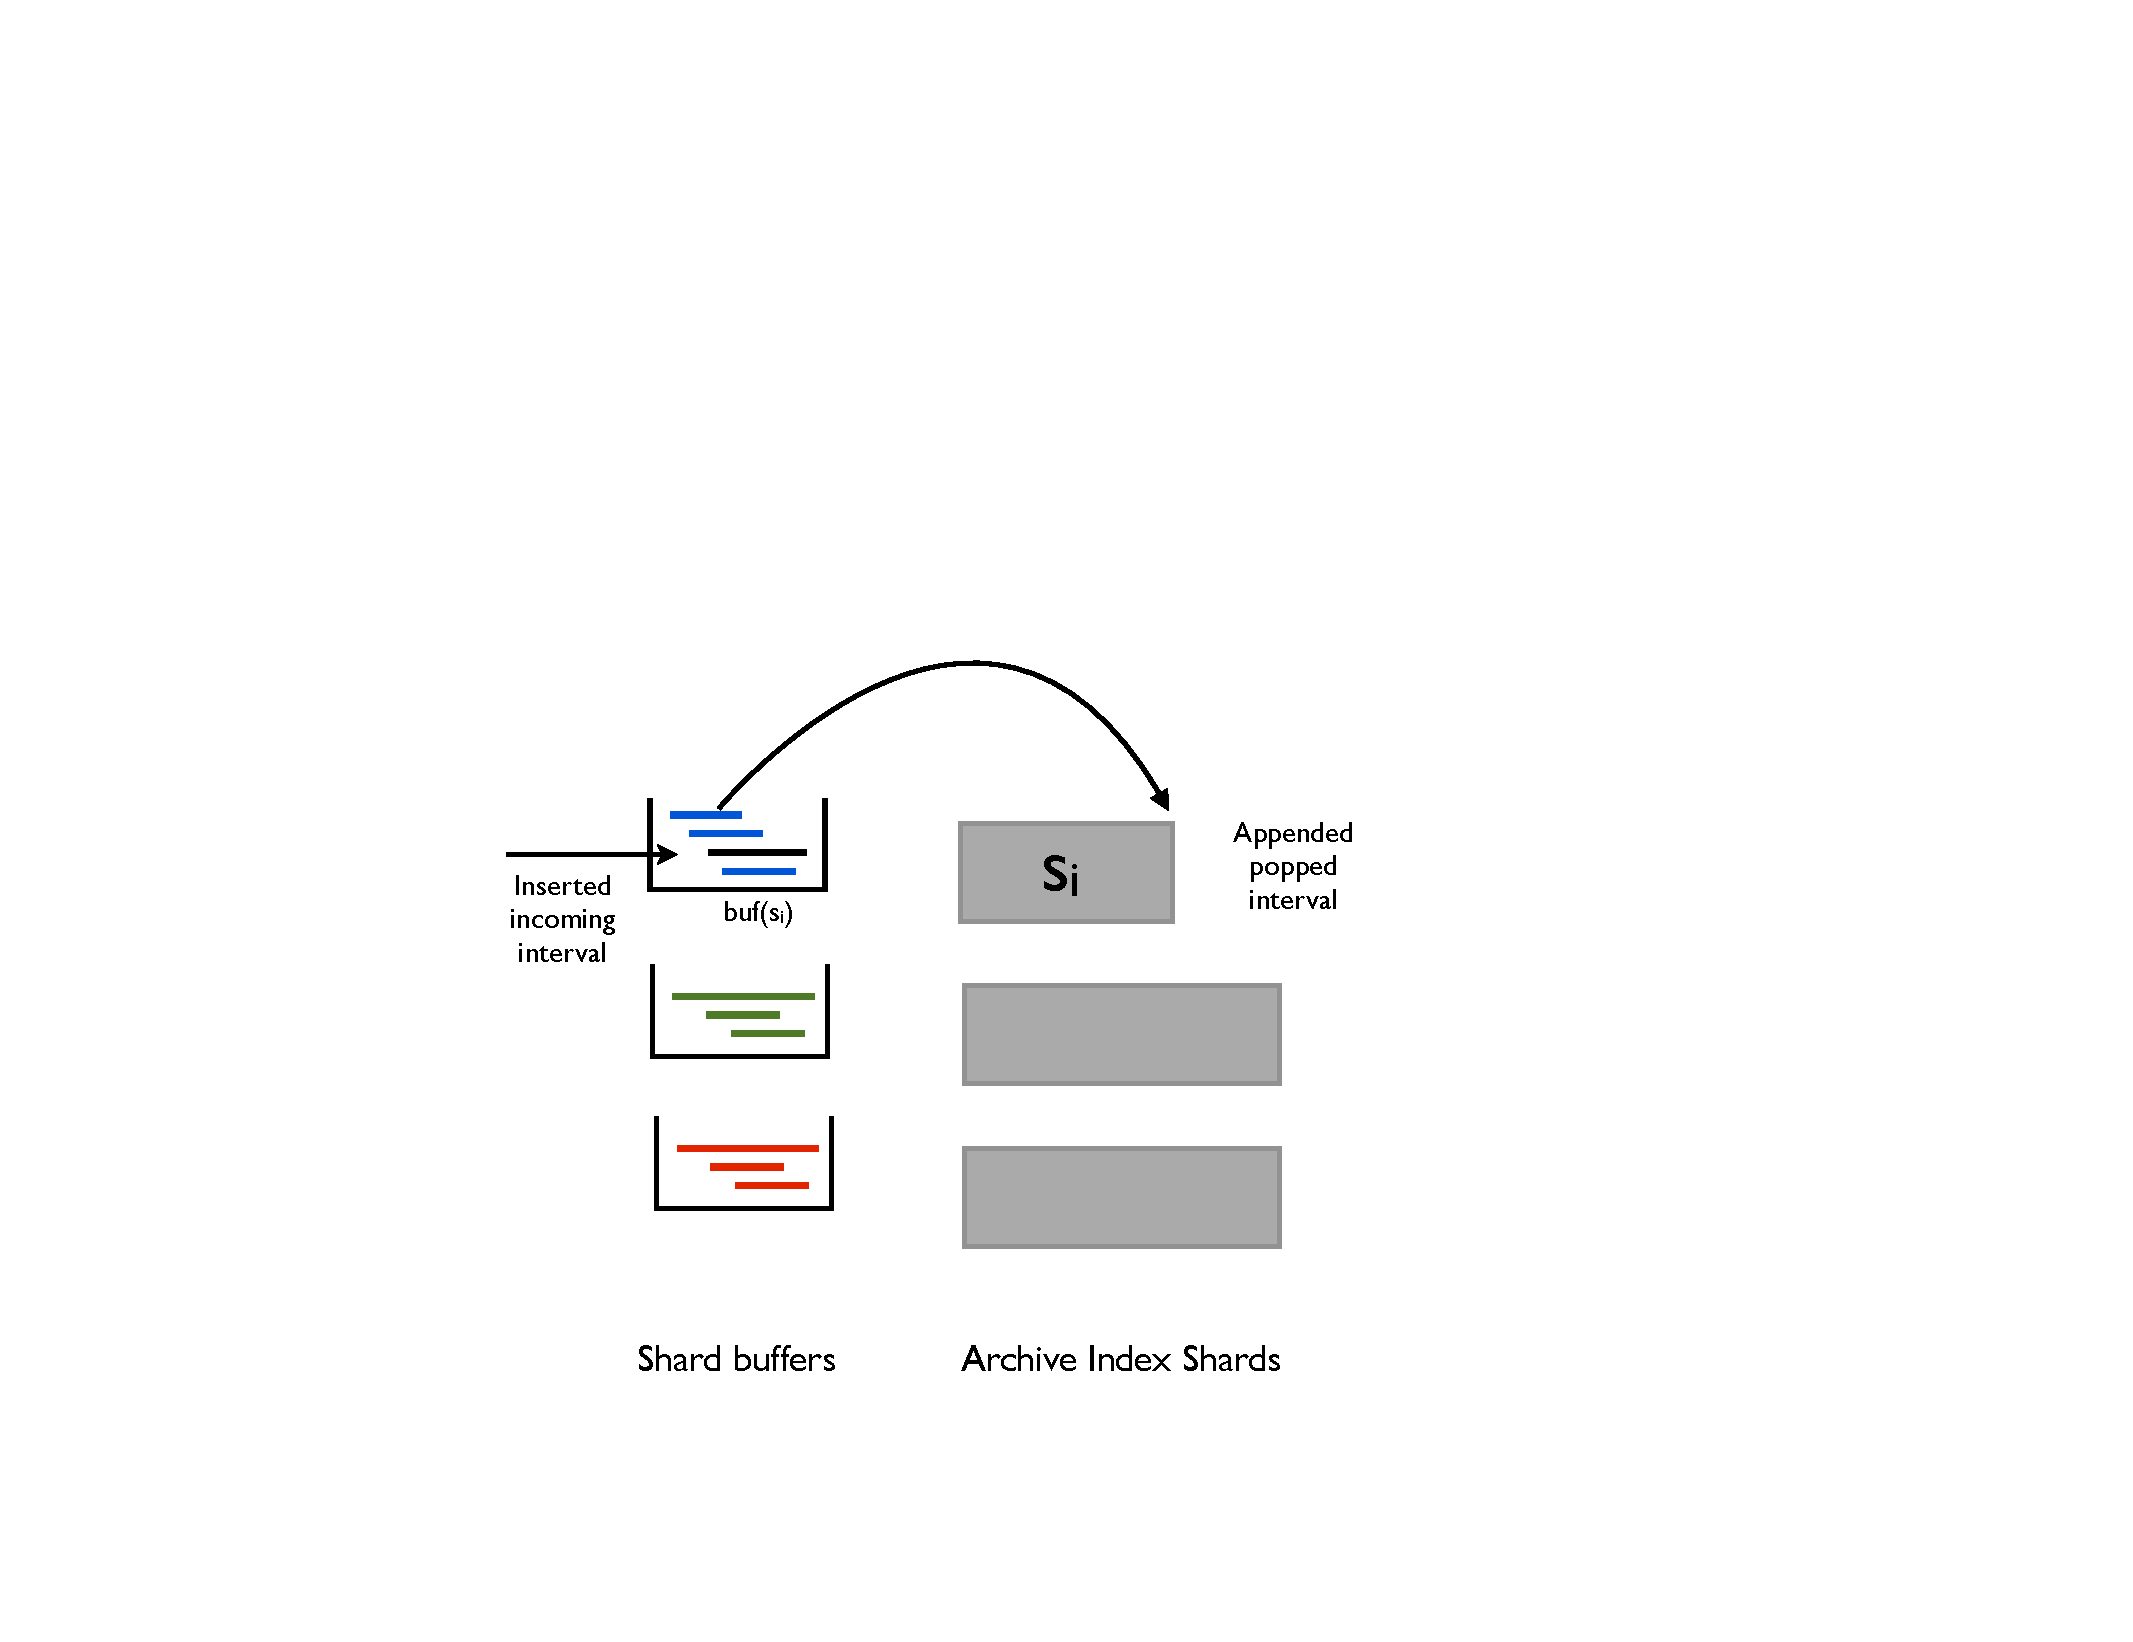
\includegraphics[width=0.475\textwidth]{resources/inc_sharding.pdf}
		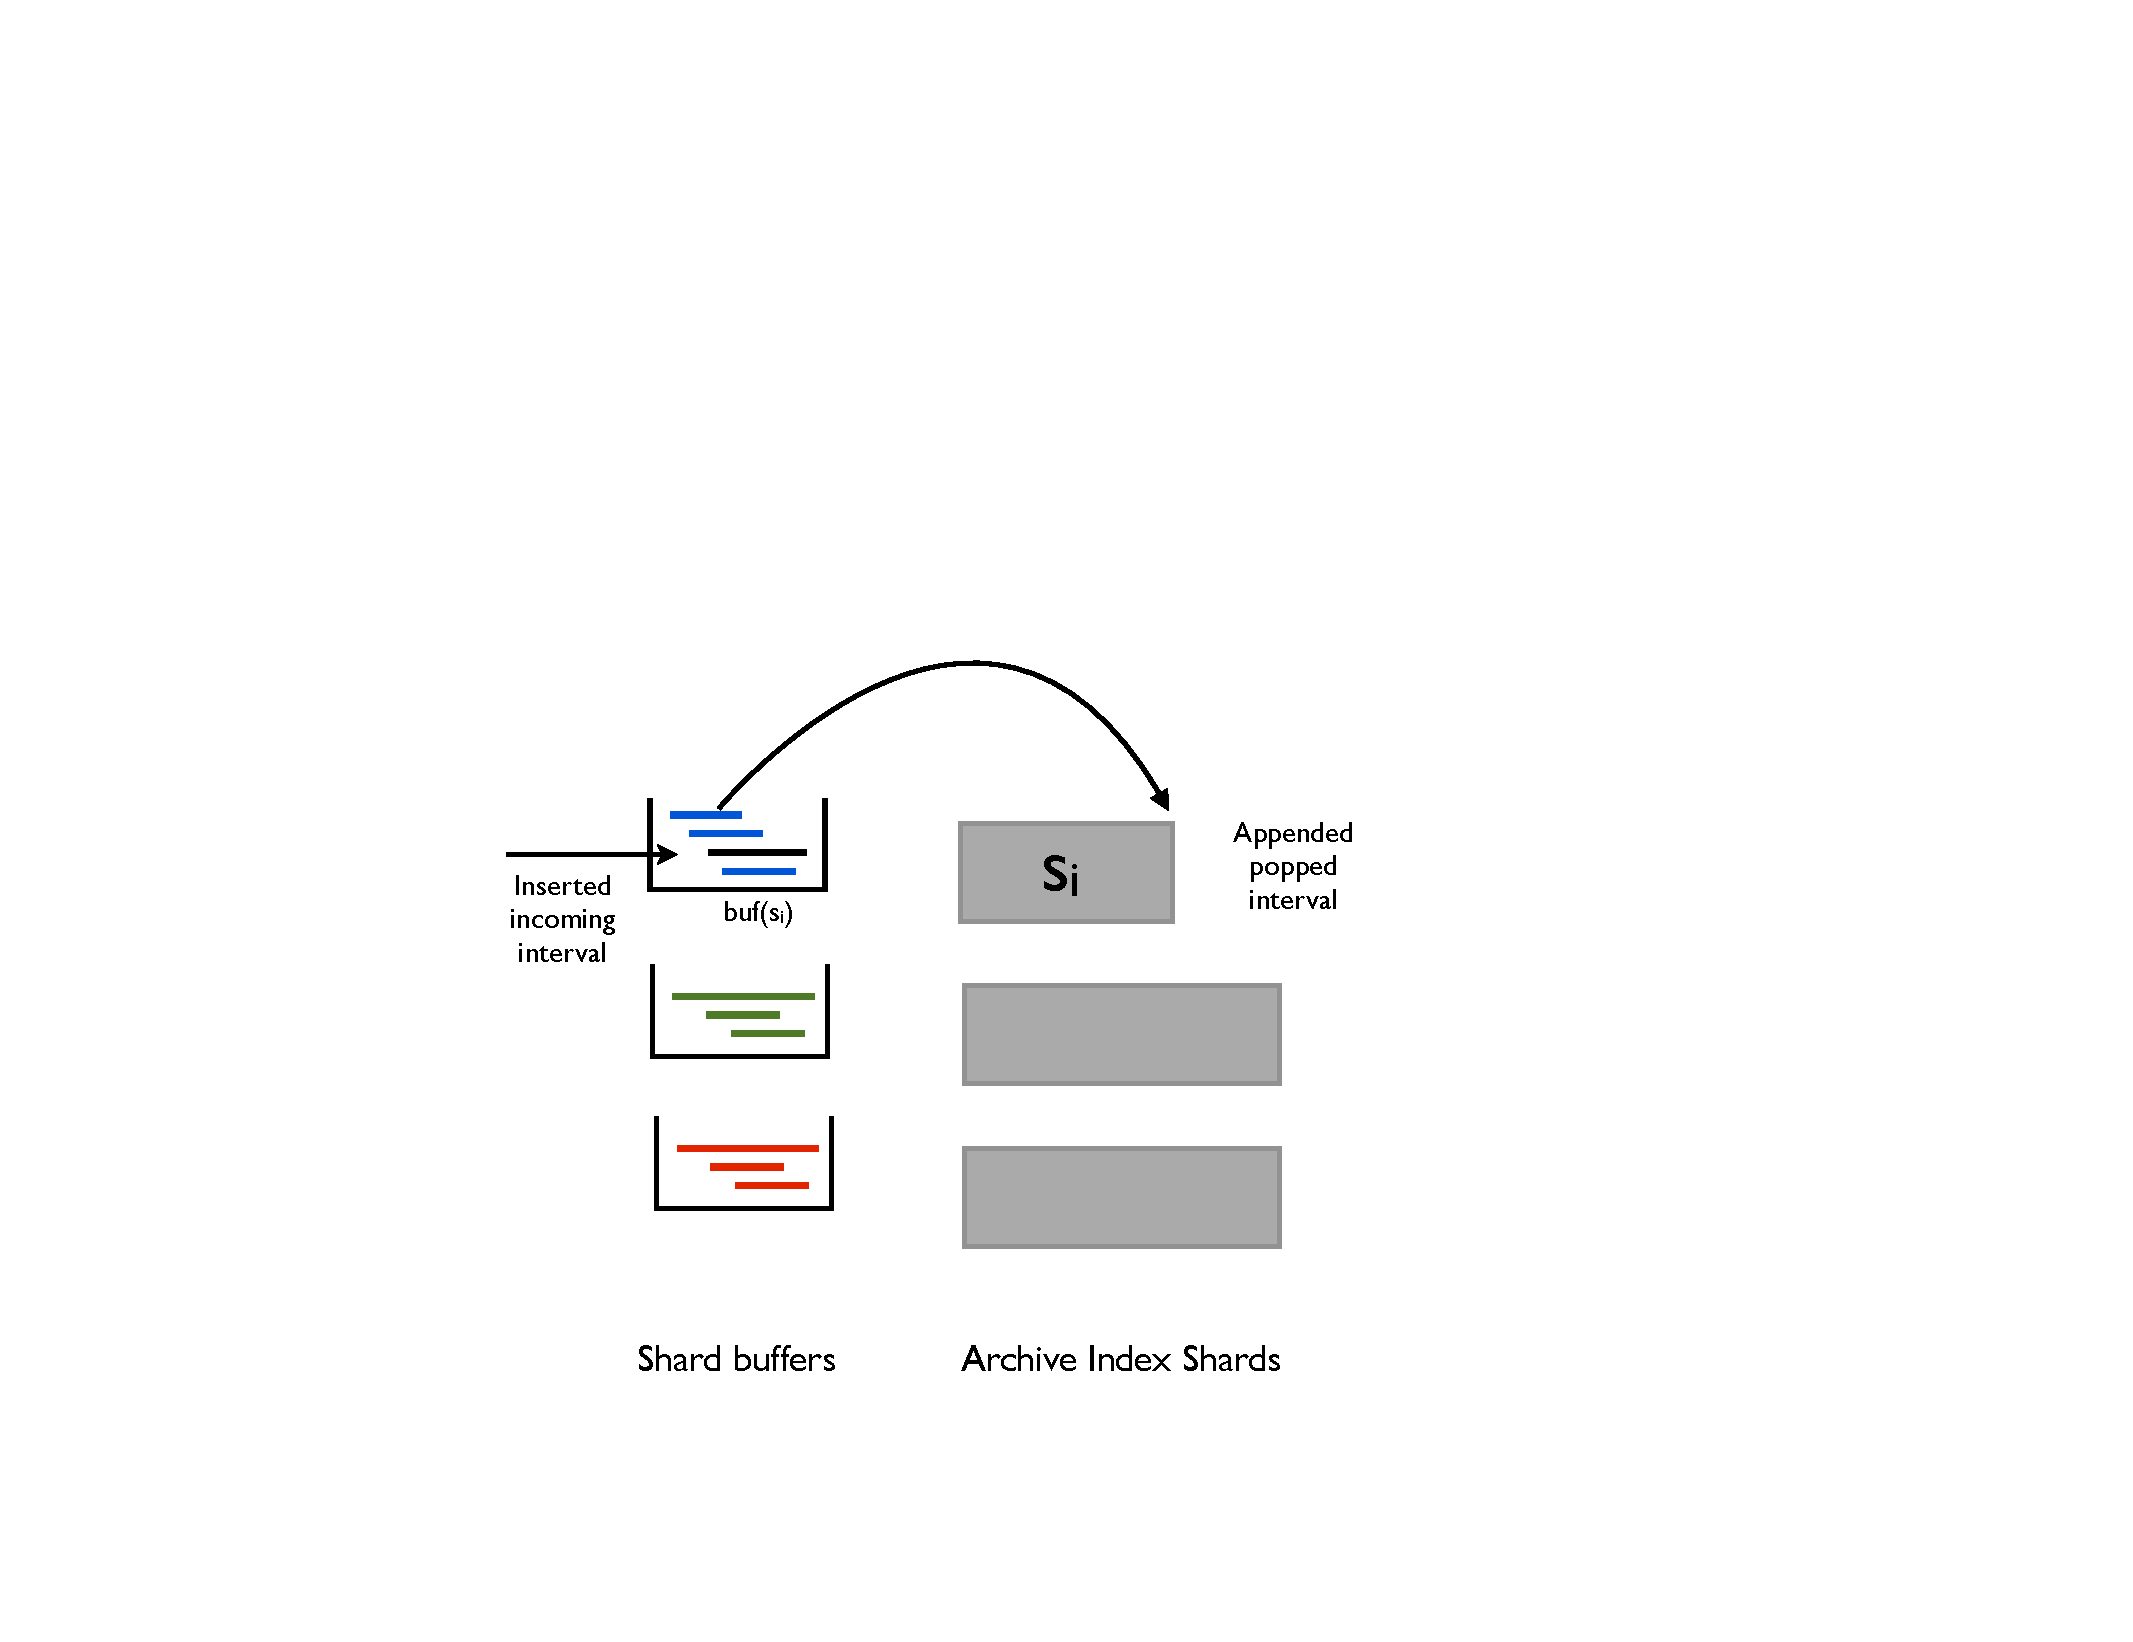
\includegraphics[width=0.475\textwidth]{resources/inc_sharding.pdf}
	\caption{Incremental sharding}
	 \label{fig:inc_sharding}
\end{figure}

The algorithm processes postings in the increasing order of end times (see line 1) and creates or updates shards incrementally. It follows a scheme of immediate assignment but deferred append of a posting to a shard. For each shard, we maintain a \emph{shard buffer} of size $\eta+1$ and a \emph{shard-begin time}. The assignment of the posting to a shard is based on the begin time of the shard and the shard buffer defers the actual writing or appending of the posting of the shard to satisfy the bounded subsumption property. In other words, the shard buffer maintains the posting until it deems it right to be appended to the end of the shard.

When a posting $L_v[i]$ is processed, it is either assigned to an existing shard based on the posting and shard-begin times (see line 15), or it results in the creation of a new shard (lines 7-10). The creation of a new shard involves setting the begin time of the shard to zero and placing the chosen posting in its shard buffer. Until the buffer reaches its capacity of $\eta$ the begin time of the shard remains zero. The shard-begin time is first updated when a posting is popped out of it after the buffer reaches its capacity $\eta+1$.  When the assignment for the posting is decided, say $\sigma_t$, it is placed in the respective shard buffer $buf(\sigma_t)$ (see line 19). The incremental sharding chooses the shard whose begin time has the least difference with the begin time of the incoming posting (see line 15). 

The shard buffers determine the relative position of the postings in the shard where it will be finally stored. The insertions into the buffer are made to preserve the begin-time order (see line 19) which in turn ensures a begin-time order when postings are removed from it. This is shown in Figure~\ref{fig:inc_sharding}. Only the first posting or the posting with the minimum begin time is removed from the buffer to limit the buffer size to $\eta + 1$ (line 23) and it is appended to the end of its corresponding shard $\sigma_t$. The shard buffers also ensure that no posting in a shard subsumes more than $\eta$ postings. This is done by setting the begin time of a shard $\sigma_t.begin$ to the first posting $begin(first(buf(\sigma_t)))$(or the posting with the least begin time) of the shard buffer as in line 24. The posting with the minimum begin time in the shard can subsume the maximum number of postings and any posting with a begin time lesser than it is disallowed.

Note that the use $\cup$ in lines 23 and 30 indicates the \emph{append} operation on the shard that is logically organized as a list of postings in their begin-time order.


% Observe that  operator $\cup$ used might be misleading in lines 23 and 30. We intend an append operation to the shard that is logically organized as a list of postings in their begin-time order.
\subsection{Approximation Guarantee for Incremental Sharding}
\label{proof:approx_guarantee}

\begin{theorem}
\label{thm:inc_sharding}  
Incremental sharding is a $(2- \frac{2}{\eta+2})$ approximation.
\end{theorem}

We use the following lemmas to prove the theorem.
Assuming that incremental sharding produces $m$ shards, we first construct a worst case scenario. For notational convenience let us assume that shards are numbered according to their creation times in incremental sharding, i.e., $\sigma_1$ was created before $\sigma_2$ and so on. 

\begin{lemma}[Descending Begin Times]
\label{lem:descending_begintimes}
If incremental sharding created a shard $\sigma_{i+1}$ after $\sigma_i$, then $\sigma_i.begin > \sigma_{i+1}.begin$.
\end{lemma}
\begin{proof}{}
	We prove this property by induction over increasing number of postings $p_i \in L_v$ which are added in in end-time order, i.e, $end(p_{i+1}) \, > \, end(p_{i})$ .

	$\mathbf{i = 1:}$ For the first posting $p_1$ the property holds since there are no earlier shards.

	$\mathbf{i \rightarrow i+1}$: Let there be $n$ existing shards $\mathcal{S} = \{ \sigma_1 \cdots \sigma_n \}$. Depending on the begin time of the $(i+1)$-th posting $begin(p_{i+1})$ we consider the following two cases:

	\textbf{Case 1:} If $begin(p_{i+1}) < \sigma_k.begin \,\, , \,\, 1 \le k \le n$, then $p_{i+1}$ forms a new shard $\sigma_{new}$ and the begin of the shard $\sigma_{new}.begin$ is less than all the existing shard-begin times. This proves the claim.

	\textbf{Case 2:} Assuming $\exists \sigma_k : begin(p_{i+1}) \geq \sigma_k.begin$ and on addition of $p_{i+1}$ to $\sigma_k$ there is a violation of the descending begin-time order of shards, i.e., $\sigma_k.begin > \sigma_{k-1}.begin$. This means that $\sigma_{k-1}.begin < begin(p_{i+1})$ and $p_{i+1}$ should have been assigned to $\sigma_{k-1}$ due to a smaller difference according to the induction hypothesis of $\sigma_{k+1}.begin > \sigma_{k}.begin\,\,, \,\,\forall 1 \le k < n$.
\end{proof}

\begin{lemma}[Incremental Subsumption]
\label{lem:incremental_subsumption}
	A posting added to $\sigma_i$ subsumes at least $(i-1)(\eta + 1)$ postings.
\end{lemma}


\begin{lemma}[Incremental Subsumption]
\label{lem:incremental_subsumption}
	The number of postings subsumed a posting added to $\sigma_i$ is at least $(i-1)(\eta + 1)$.
\end{lemma}

\begin{proof}{}
	Note that $\sigma_i.begin$ refers to the time of the first posting in the buffer of shard $\sigma_i$ or the earliest begin time in the shard buffer $buf(S)$. 
	
	By Lemma~\ref{lem:descending_begintimes} we know that there is an ordering of the shard-begin times. Hence for a posting $p$ assigned to $\sigma_i$ the following holds -- $begin(p) < \sigma_{i-1}.begin < \cdots < \sigma_1.begin$. Since we assume end-time arrival order of postings, it subsumes all postings in $i-1$ shards buffers, which are $\sigma_1,...,\sigma_{i-1}$. Further the fixed buffer size of $\eta+1$ results in making the subsumptions lower bounded by $(i-1)(\eta + 1)$.\end{proof}

We now introduce the notion of \emph{stalactite groups}, building on the notion of the \emph{Stalactite set} $\Upsilon$ according to the definition~\ref{def:stalactite}. Formally,

\begin{definition}[Stalactite Groups]
A shard $\sigma$ is said to be exhibit stalactite grouping if we can partition the shard into sets of postings called groups $G$ such that  for groups $s_i, s_j \in \sigma$ and $i<j$ the following holds:
$$
	q \sqsupset p , \,\,\,\, \forall p \in s_i, \forall q \in s_j.
$$
\end{definition}

In other words, \emph{stalactite groups} (see Figure~\ref{fig:stalactite_groups}) in a shard is the organization of postings into groups such that choosing one posting from each group results in a \emph{stalactite set}.

\begin{lemma}[Stalactite Grouping]
\label{lemma:stalactite_grouping}
	Stalactite grouping with a staircase property in each shard is the worst case for incremental sharding.
\end{lemma}

\begin{proof}{}
	From the previous lemma, any input resulting in $m$ shards from incremental sharding will have at least postings with $\eta+1$, $2(\eta+1)$, $\cdots$, $(m-1)(\eta+1)$ subsumptions in $\sigma_2, \sigma_3, \cdots, \sigma_m$ respectively. Let us suppose that the set of subsumed postings when the first posting added to $\sigma_i$ be represented as $sub(\sigma_i)$. To reduce the overall number of shards we should strive for a configuration with a minimum number of subsumptions. This is possible when $sub(\sigma_1) \subseteq sub(\sigma_2) \subseteq \cdots \subseteq sub(\sigma_m)$ and $|\sigma_i| = \eta + 1, \forall i = 1,\ldots,m$. This arrangement forms a \emph{stalactite group} (see Figure~\ref{fig:stalactite_groups}) with each of the groups having a cardinality of $\eta+1$.


	Additionally, each of these stalactite groups should have a staircase arrangement to allow for the maximum capacity - $\eta$ - out-of-place insertions. Any additional posting or misaligned posting either increases subsumption or reduces capacity for out of place insertions. Any removal of postings on the other hand result in contradiction to the original assumption that there are $m$ shards from incremental sharding.
\end{proof}


\begin{figure}[tb]
  	\centering
		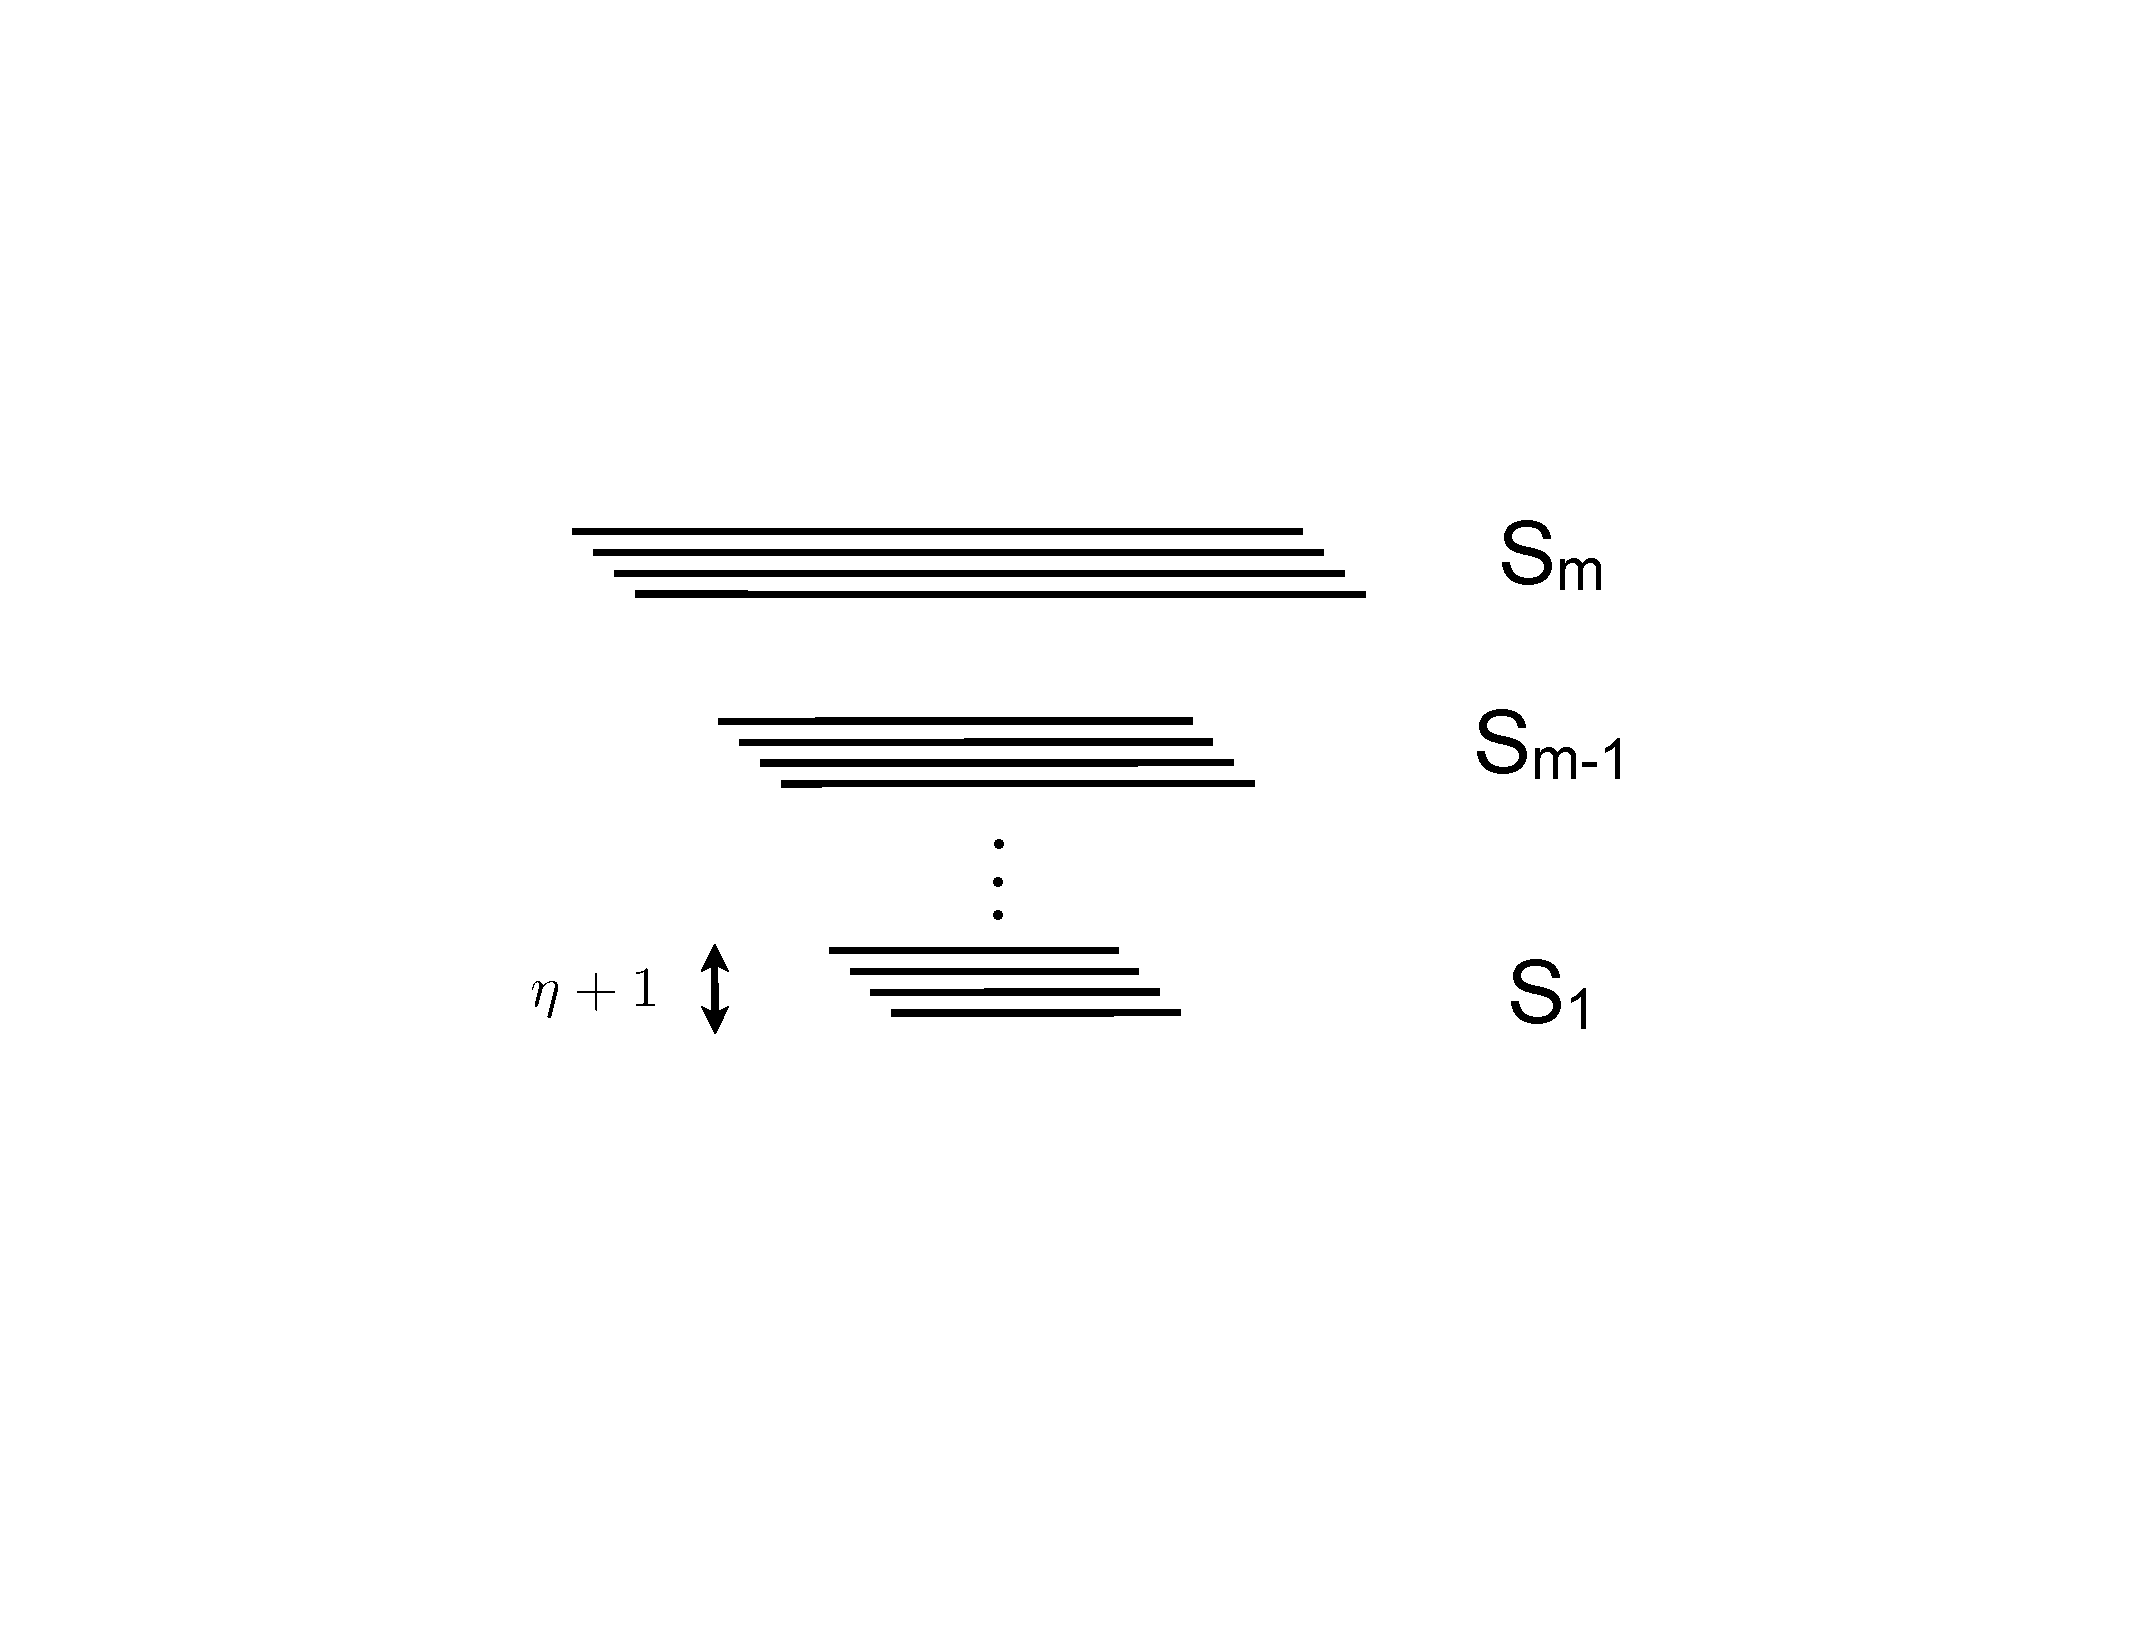
\includegraphics[width=0.375\textwidth]{resources/stalagtite_grp.pdf}
   	\caption{Stalactite groups}
		  \label{fig:stalactite_groups}	
\end{figure} 

Now we can complete the proof for Theorem 1.%~\ref{thm:inc_sharding}.

\begin{proof}{}
	From the Lemma~\ref{lemma:stalactite_grouping} we know that there are $m$ stalactite groups with each group residing in the shards formed from incremental sharding. It is easy to see that none of the optimal shards will have more than $2\eta + 1$ postings. Thus we choose an assignment where we try to minimize the number of shards, i.e., choose as many shards with $2\eta + 1$ postings as possible. One such assignment is when we assign $\eta$ of the $\eta+1$ postings of $\sigma_i$ to $\sigma_{m+1-i}, \,\, \forall i \leq \frac{m}{2}$. The remaining $\frac{m}{2}$ postings (a posting from each $\sigma_i$) can then be placed in $\frac{m}{2(\eta+1)}$ shards. Hence for $m$ shards created by incremental sharding  we get a minimum of $\frac{m}{2} + \frac{m}{2(\eta+1)}$ shards. Notice that we can have other arrangements which give the same number of minimum shards. The ratio 

	$$
		\frac{|S|}{OPT} = \frac{m}{\frac{m}{2} + \frac{m}{2(\eta+1)}} 
						= 2 \left(1 - \frac{1}{\eta + 2}\right)
	$$

	proves that incremental sharding is a factor $(2  -  \frac{2}{\eta+2})$ approximation algorithm.
\end{proof}

% System Architecture

%!TEX root = ./sigir2011.tex
\section{System Architecture}
\label{chap:sharding:sec:system}

Figure~\ref{fig:archive_indexing_system} shows a high-level overview
of the architecture of a search engine using our incremental sharding
method. It consists of
\begin{itemize}
\item the \emph{active index} for all active versions of documents,
  consisting of an in-memory inverted list for each term that keeps
  the active versions of documents,
\item the \emph{archive index} for all archive versions of documents,
  consisting of an inverted list for each term that is organized in
  shards. The archive index consists of an in-memory index \emph{IMAI}
  and an on-disk index \emph{EMAI}, both organized in shards.
\item A \emph{crawler} that continuously crawls the target Web sites,
  for example, a predefined set of domains or the complete Web.
\end{itemize}

When the crawler encounters a new document that has been unknown so
far, it adds it to the active index; this is an inexpensive operation
since the active index is in main memory. When a document is found
again, it is checked for changes (using, for example, a fingerprinting
technique such
as~\cite{DBLP:journals/cn/BroderGMZ97,DBLP:conf/sigir/Henzinger06}). If
changes are detected, the active version of that document turns into
an archive version (with end time equal to the crawl time) and is
sent to the archive index, and postings for the new active
version are added to the active index.

The archived version is then added to the in-memory archive index by
first creating the corresponding postings for each term, which are
then added to the in-memory archive index using the incremental
technique from
Section~\ref{chap:sharding:sec:inc_sharding}. Figure~\ref{fig:finalizing_versions}
shows an example for this, where in a crawl at time $t_{now}$ a new
version $d_4^3$ for document $d_4$ is detected. This results in firstly
adding a new version $d_4^3$ with a begin time $t_{now}$ to the
affected terms in the active index. Secondly, the end time of $d_4^2$ is
finalized and the posting $\langle d_4^2, [t_1, t_{now}], \, score
\,\rangle$ with the complete posting information is sent to the
archive indexing system. In the archive indexing system this posting
is processed by placing it in the shard buffer of term ``v" and
updating the IMAI from the popped posting in the buffer as shown in
Figure~\ref{fig:inc_sharding}. As soon as the in-memory index IMAI is
full, postings are merged into the disk-based archive index EMAI,
merging corresponding shards; this essentially corresponds to
incremental maintenance of standard inverted lists.

\begin{figure}[tb]
  	\centering
	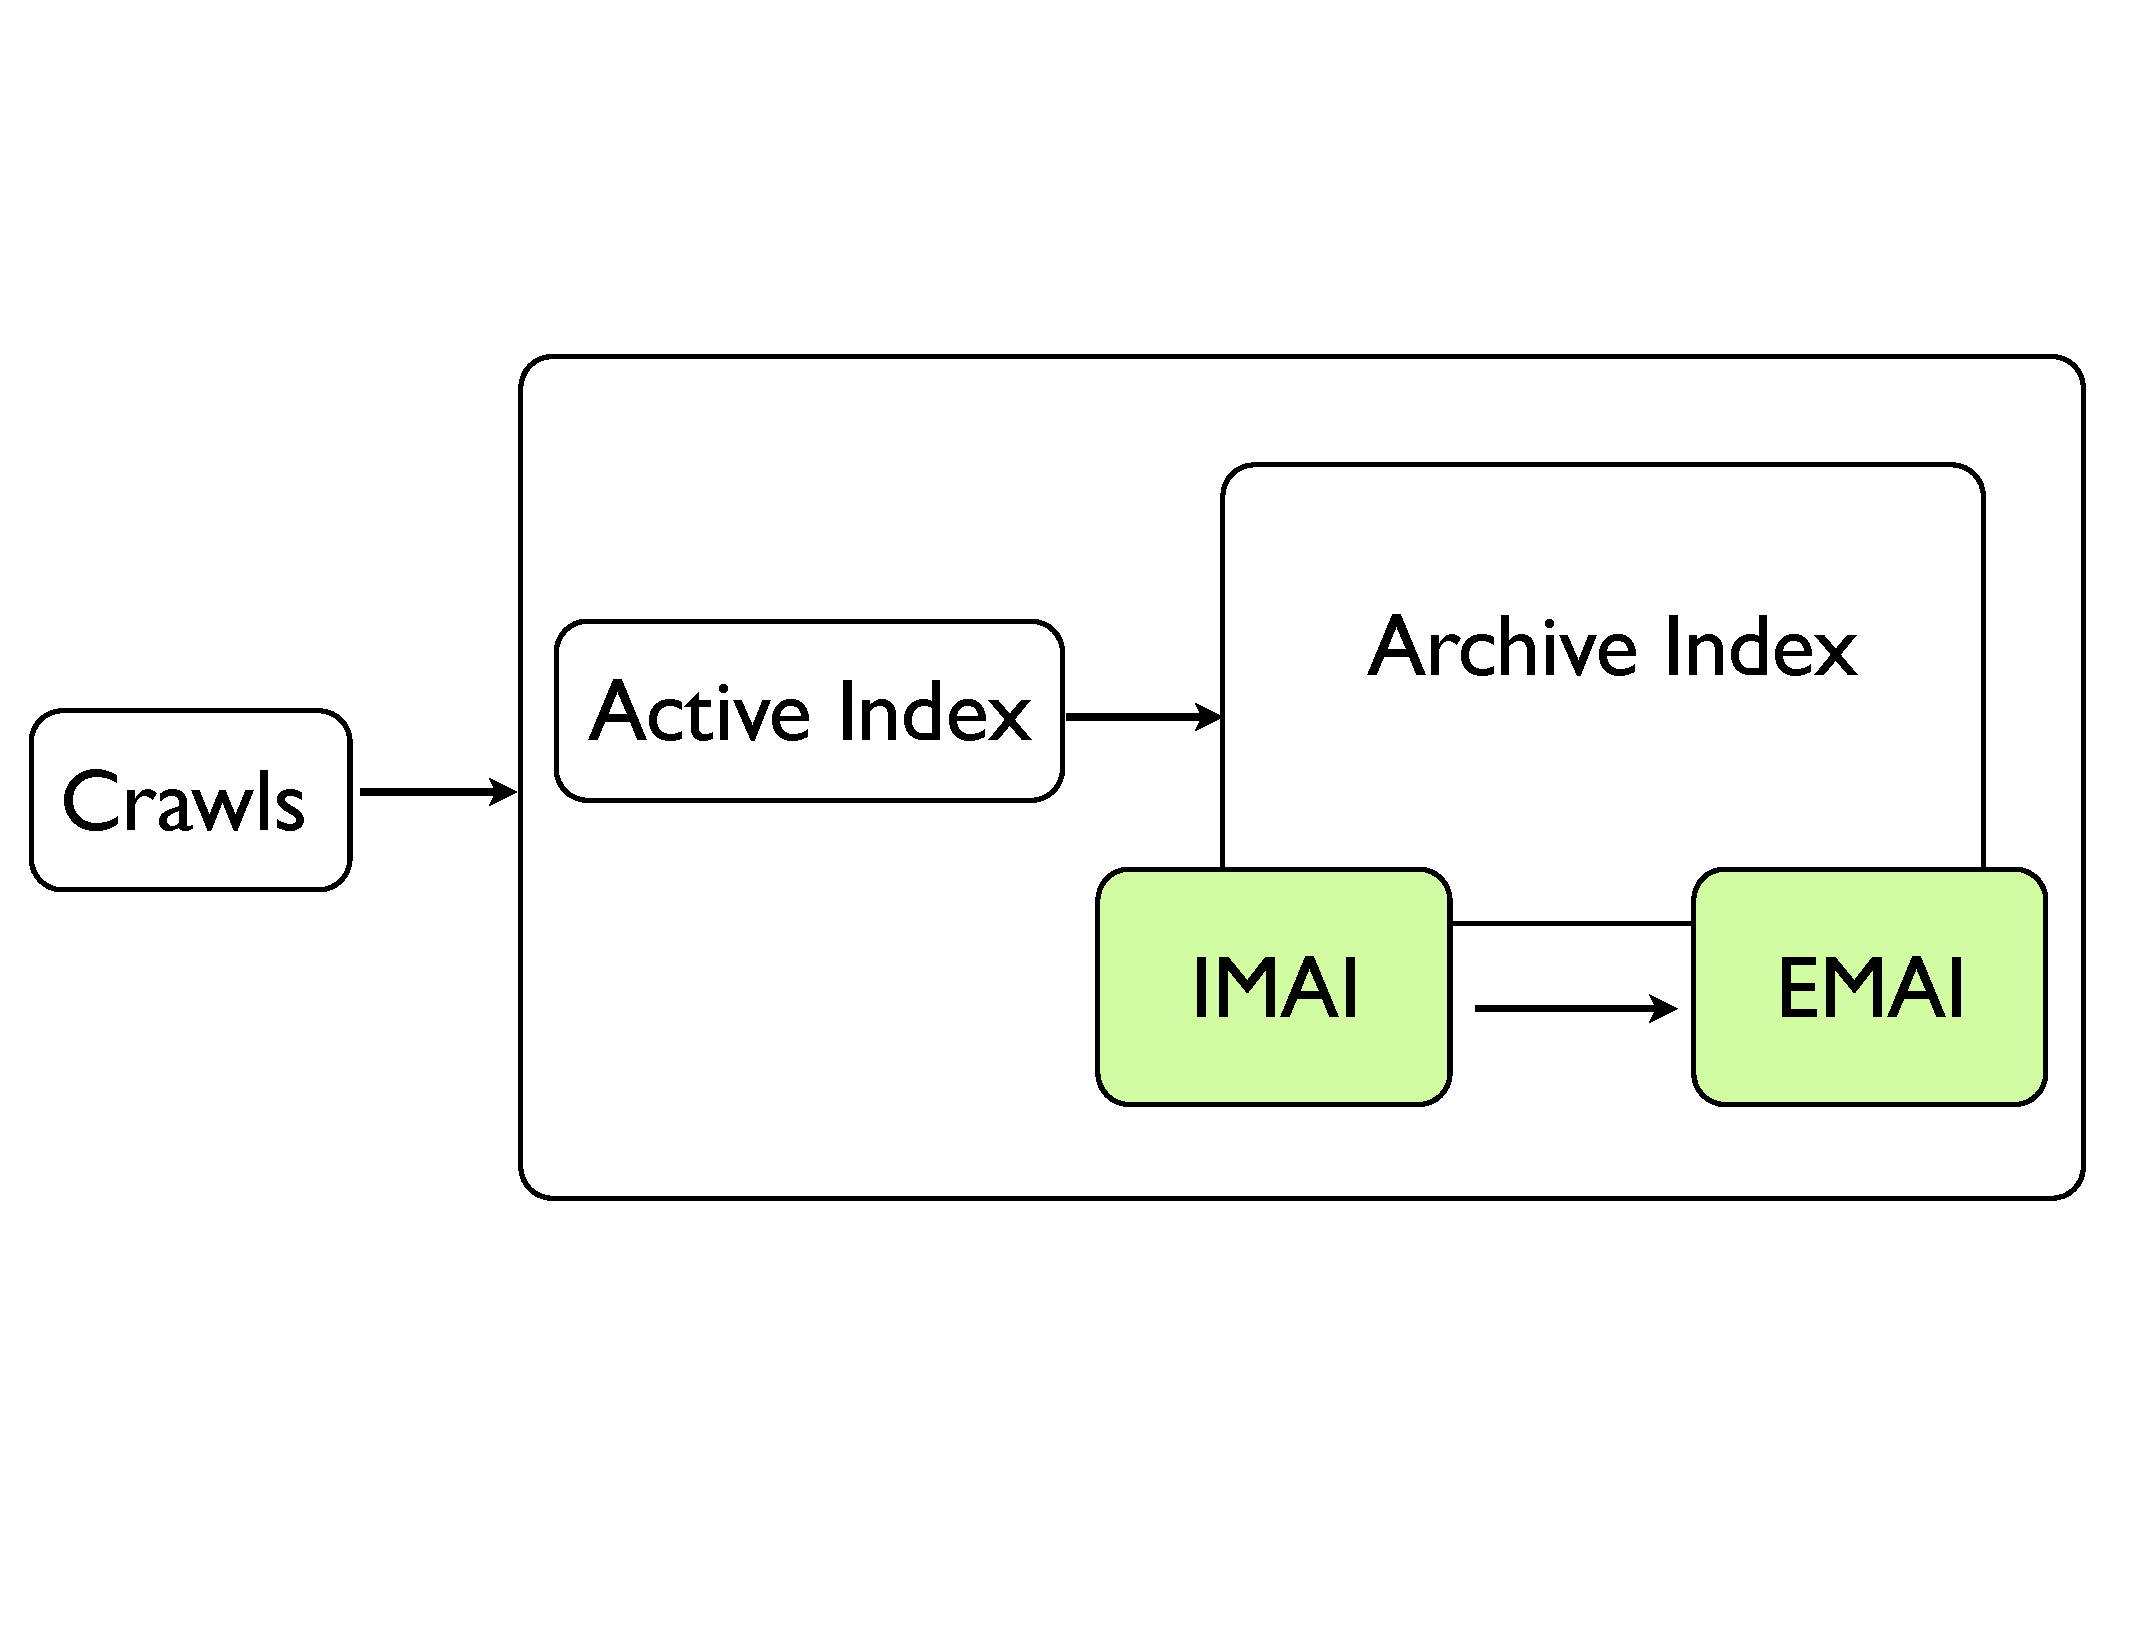
\includegraphics[width=0.5\textwidth]{resources/system_arch_incsh.pdf}
   	\caption{System architecture}
		  \label{fig:archive_indexing_system}	
\end{figure}

% Experimental Evaluation

\section{Experimental Evaluation}
\label{chap:sharding:sec:eval}

In this section, we describe our experimental evaluation of index sharding. We first present our experimental setup, datasets, and workloads used. We then examine in detail the impact of all indexing methods considered on query processing, index sizes and index maintenance. 

\subsection {Setup}
 All experiments were conducted on Dell
PowerEdge M610 servers with 2 Intel Xeon E5530 CPUs, 48 GB of main
memory, a large iSCSI-attached disk array, and Debian GNU/Linux (SMP
Kernel 2.6.29.3.1) as operating system. Experiments were conducted
using the Java Hotspot 64-Bit Server VM (build 11.2-b01). 

\subsection{Datasets Used}
For our experiments we use the following two real-world datasets WIKI and UKGOV. The characteristics of these datasets are detailed below and summarized in Table~\ref{tab:datasets}.

\begin{table*}
  \center
  \begin{tabular}{l c c r r r} 
      \toprule
      { Dataset} & \multicolumn{1}{c}{Coverage}&  \multicolumn{1}{c}{Size (in GB)} & \multicolumn{1}{c}{$\mathcal{N}$} & \multicolumn{1}{c}{$\mathcal{V}$} & \multicolumn{1}{c}{$\mu / \sigma$}\\
      \midrule
      {\bf WIKI} & 2001  to 2005  & $\sim$700 & 1,517,524 & 15,079,829 & 9.94 / 46.08\\

      {\bf UKGOV} & 2004 to 2005 & $\sim$400 & 685,678 & 17,297,548 & 25.23 / 28.38\\
      \bottomrule
    \end{tabular}\\
    % fluca
  \caption{Characteristics of datasets used}
  \label{tab:datasets}
\end{table*}

\begin{enumerate}
\item[\textbf{WIKI}]
%\noindent\textbf{WIKI.}
{The \emph{English Wikipedia Revision History}
    \cite{wiki}, whose uncompressed raw data amounts to 0.7~TBytes,
    contains the full editing history of the English Wikipedia from
    January~2001 to December~2005. We indexed all versions of
    encyclopaedia articles excluding versions that were marked as the
    result of a minor edit (e.g., the correction of spelling errors
    etc.). This yielded a total of 1,517,524 documents with 15,079,829
    versions having a mean ($\mu$) of 9.94 versions per document at
    standard deviation ($\sigma$) of 46.08.}
    
\item[\textbf{UKGOV}]
%\noindent\textbf{U.K.GOV.}
  { This is a subset of the European Archive~\cite{ea}, containing
    weekly crawls of eleven governmental websites from the U.K. We
    filtered out documents not belonging to MIME-types
    \texttt{text/plain} and \texttt{text/html} to obtain a dataset
    that totals 0.4~TBytes. This dataset includes 685,678 documents
    with 17,297,548 versions ($\mu = $ 25.23 and $\sigma = $ 28.38).}
%\item[NYT]}
    
\end{enumerate}

These two datasets represent realistic classes of
time-evolving document collections. WIKI is an explicitly versioned
document collection, for which all its versions are known. UKGOV is an
archive of the evolving Web, for which, due to crawling, we have only
incomplete knowledge about its versions. The incomplete knowledge can be attributed to inability to capture some versions in between crawls and inability to determine with certainty the version valid-times. For ease of experimentation,
we rounded timestamps (in both datasets) to day granularity.


\subsection{Index Management}
 We use the following types of indexes in our experiments:

\begin{enumerate}

%\item[Sliced Indexes]
%\item[Sharded Indexes]
\item
\textbf{Sharded Index}
  { We consider idealized sharding (IS) and three variants of cost-aware shard merging (CAS) as introduced in Section~\ref{chap:sharding:sec:relaxed_part}. The parameter $\eta$ reflects the I/O cost ratio. Since the $C_r/C_s$ values of disks usually vary in the order of 100 and 1000 thus we choose the parameter for shard merging accordingly, i.e., $\eta \in \{ 10, \,100, \,1000 \}$. The corresponding indexes are denoted as CAS-10, CAS-100 and CAS-1000. The penalty function used for shard merging is based on \emph{expected wasted reads}.

   We also consider indexes created with \emph{incremental sharding} (INC) as described in Section~\ref{chap:sharding:sec:inc_sharding}, with the same parameter values for CAS, i.e., $\eta \in \{ 10, \,100, \,1000 \}$.}


\item
\textbf{Vertically-Partitioned Index}
  {As the first competitor, we consider the vertically-partitioned index, referred to as VERT from now on, that are partitioned
    following the \emph{space-bound}
    approach~\cite{kberberi:sigir2007}. The parameter $\kappa$ denotes
    the space restriction that models the maximum blowup in the index size
    relative to a non-partitioned index. For our experiments we
    consider four variants of the space-bound approaches i.e.,
    parameter values for $\kappa \in \{1.5, 2.0, 2.5, 3.0\}$. These
    variants are denoted subsequently in the text as VERT-1.5, VERT-2.0,
    VERT-2.5 and VERT-3.0.}
    

%\item[Na\"ive Unpartitioned Index]
\item
\textbf{Na\"ive Unpartitioned Index}
  { As a second competitor, we build an unpartitioned index with
    provision for impact lists over ordered begin times referred to as
    CAS-inf. This serves as a proof that our techniques are effective
    not only because of the impact list construction and a global
    begin-time order.}
\end{enumerate}    

We also evaluate the effect of temporal coalescing~\cite{kberberi:sigir2007} on index size and query
processing. To this effect we build sharded and vertically-partitioned indexes with application of temporal coalescing using a parameter
$\epsilon=0.01$. Other than that, we use the same choice of parameters
as in the experiments without temporal coalescing.


Both the vertically-partitioned indexes and the sharded indexes are stored on disk using flat files containing both the lexicon as well as the partitioned posting lists. We do not filter out stop words, nor do we apply stemming/lemmatization when indexing the above datasets. We assigned document identifiers in the order of the begin time of the document versions. For compression, we employ 7-bit encoding on d-gaps and apply \emph{temporal coalescing} whenever necessary. Note that variable-byte encoding is complementary to \emph{temporal coalescing}. We use scalar payloads and store the tf-scores as floating point numbers using eight bytes. 

At runtime, the lexicon and impact lists are read
completely into main memory, and for a given query the appropriate
partitions or shards are retrieved from the index flat file on disk.

\subsection{Query Workloads and Execution}
\label{sec:sharding_workloads}
We compiled two dataset-specific query workloads by extracting
frequent queries from the AOL query logs, which were temporarily made
available during 2006. For the WIKI dataset we extracted 300 most
frequent queries which had a result click on the domain
\texttt{en.wikipedia.org} and similarly for UKGOV we compiled 50
queries which had result click on \texttt{.gov.uk} domains. Both the
vertically-partitioned and sharded index structures are built for terms specific to
the query workload. Using these keyword queries, we generated a
time-travel query workload with five instances each for the following four
different temporal predicate granularities: day, month, year and
queries spanning the full lifetime of the respective document
collection. Hence, the workload comprised of 6000 time-travel queries for WIKI and 1000 queries for UKGOV.

For query processing, we employed conjunctive query semantics, i.e.,
query results contain documents that include all the query terms. We
use wall-clock times (in milliseconds) to measure the query-processing
performance on warm caches using only a
single core. Specifically, each query was executed five times in
succession and the average of the last four runs was taken for a more
stable and accurate runtime measurement.

\section{Experimental Results}
\label{chap:sharding:sec:expt}

\begin{figure*}[tb]
  	\centering
	  \subfigure[Wikipedia]{\label{fig:wiki_query_times_daily}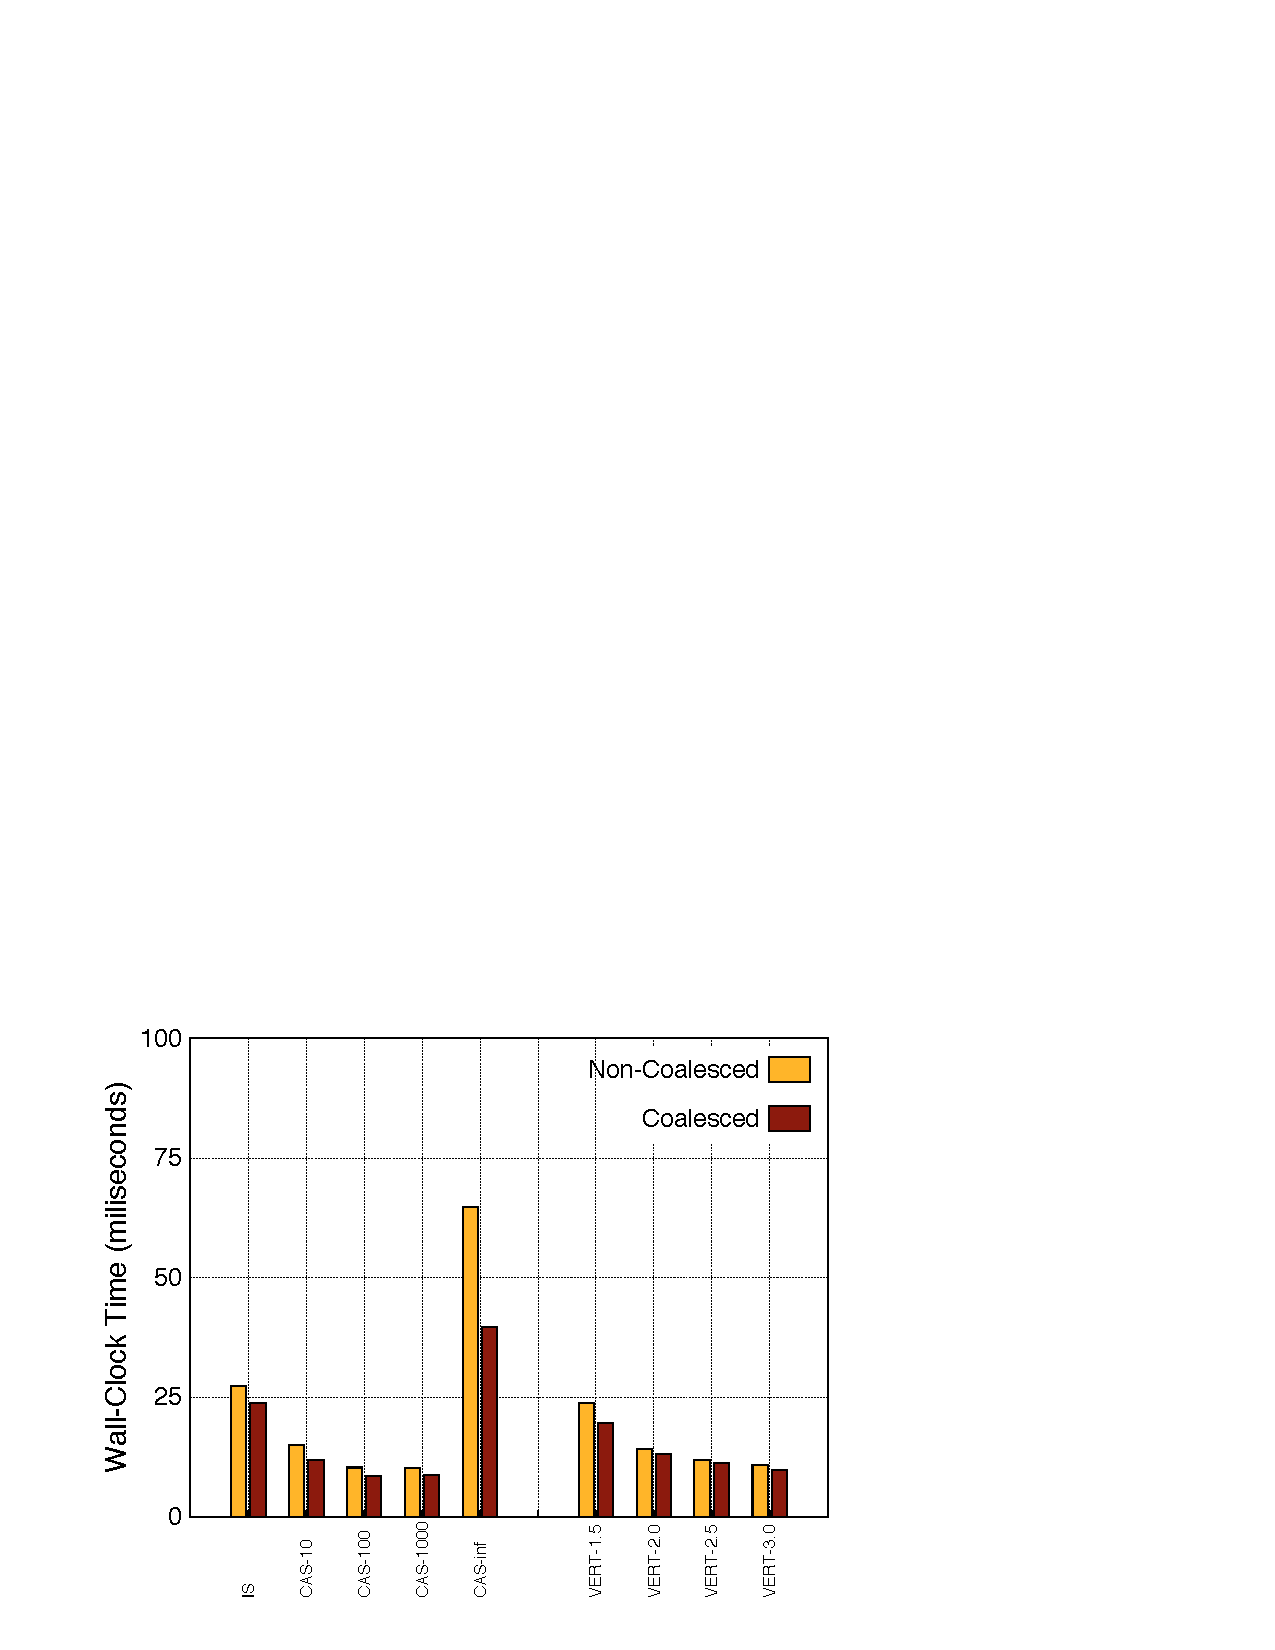
\includegraphics[width=0.5\textwidth]{plots/sharding/daily-wikipedia.pdf}}
	  \quad
	  \subfigure[UKGOV]{\label{fig:ukgov_query_times_daily}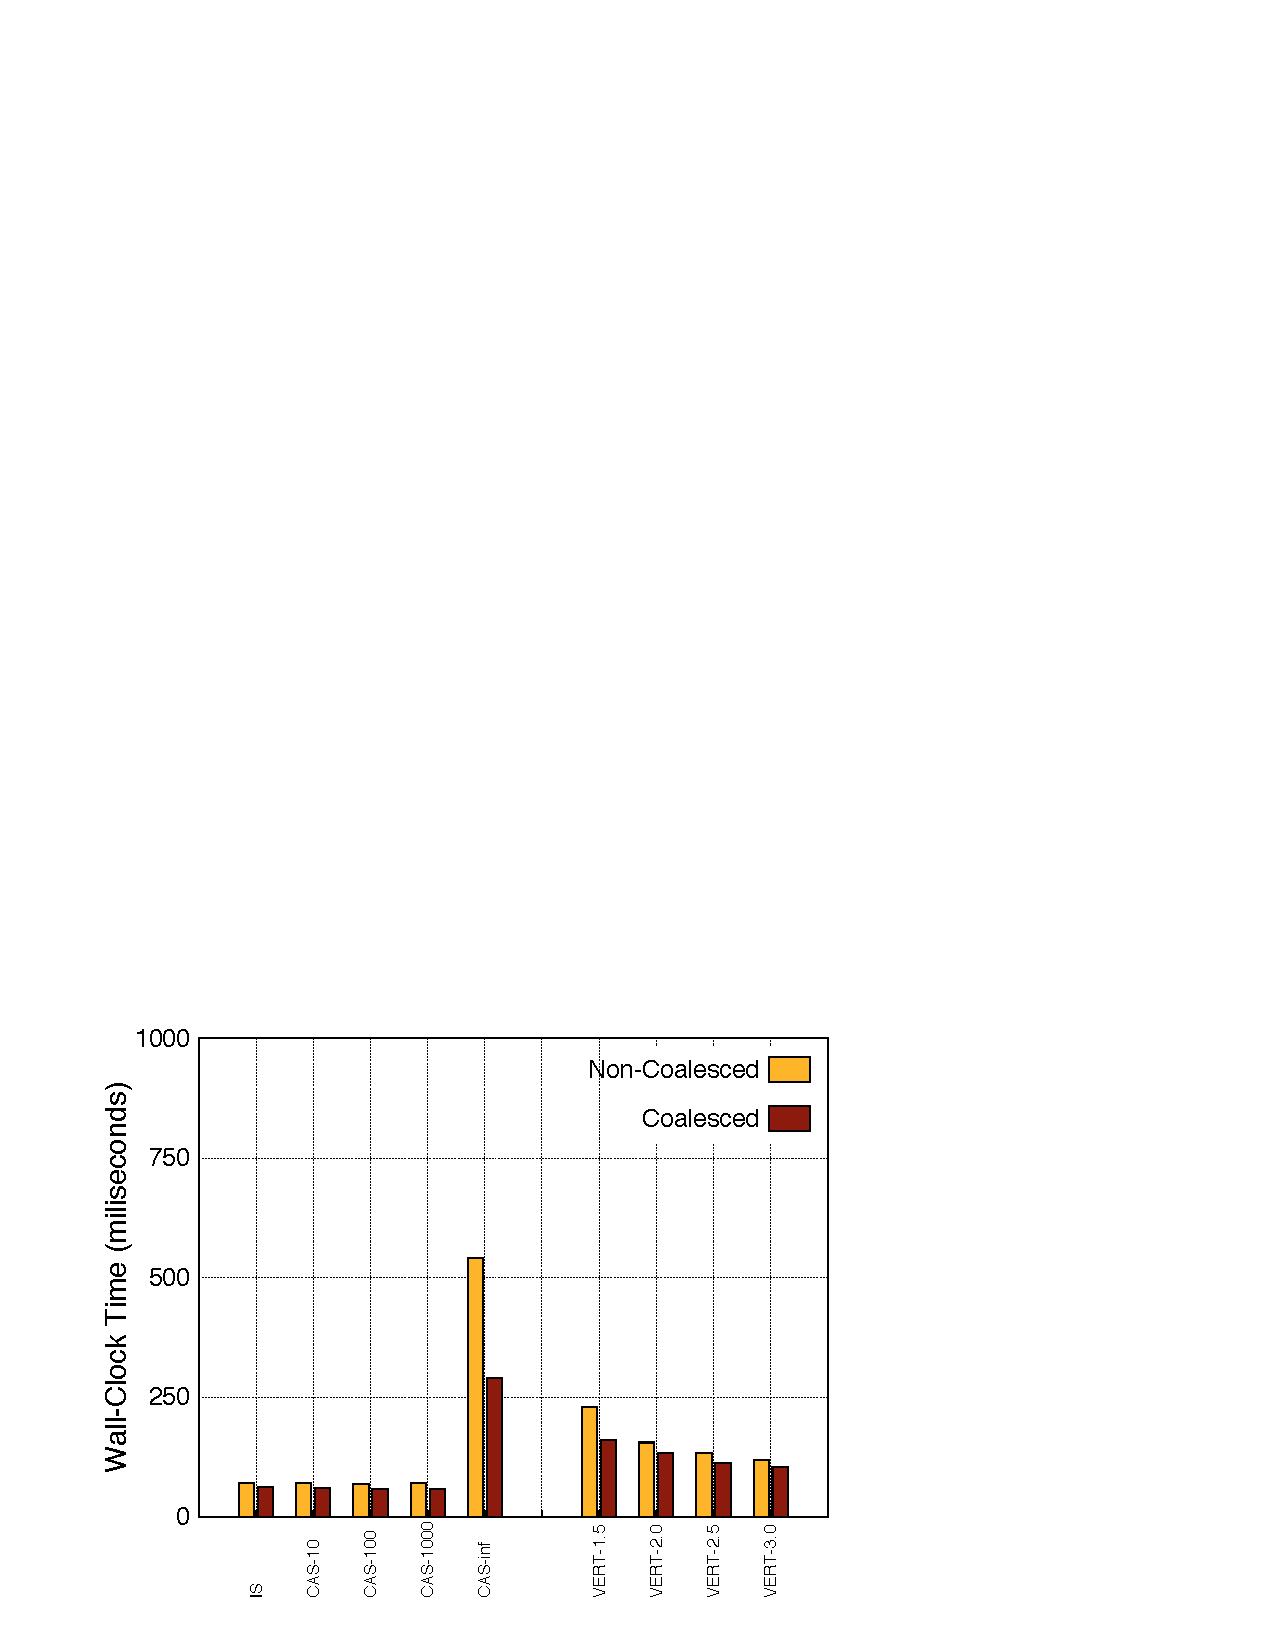
\includegraphics[width=0.5\textwidth]{plots/sharding/daily-ukgov.pdf}}
   	\caption{Wall-clock times for day-granularity queries}
\label{fig:sharding_qp_cas_vert_day}
\end{figure*}

\begin{figure*}[tb]
  	\centering
	  \subfigure[Wikipedia]{\label{fig:wiki_query_times_monthly}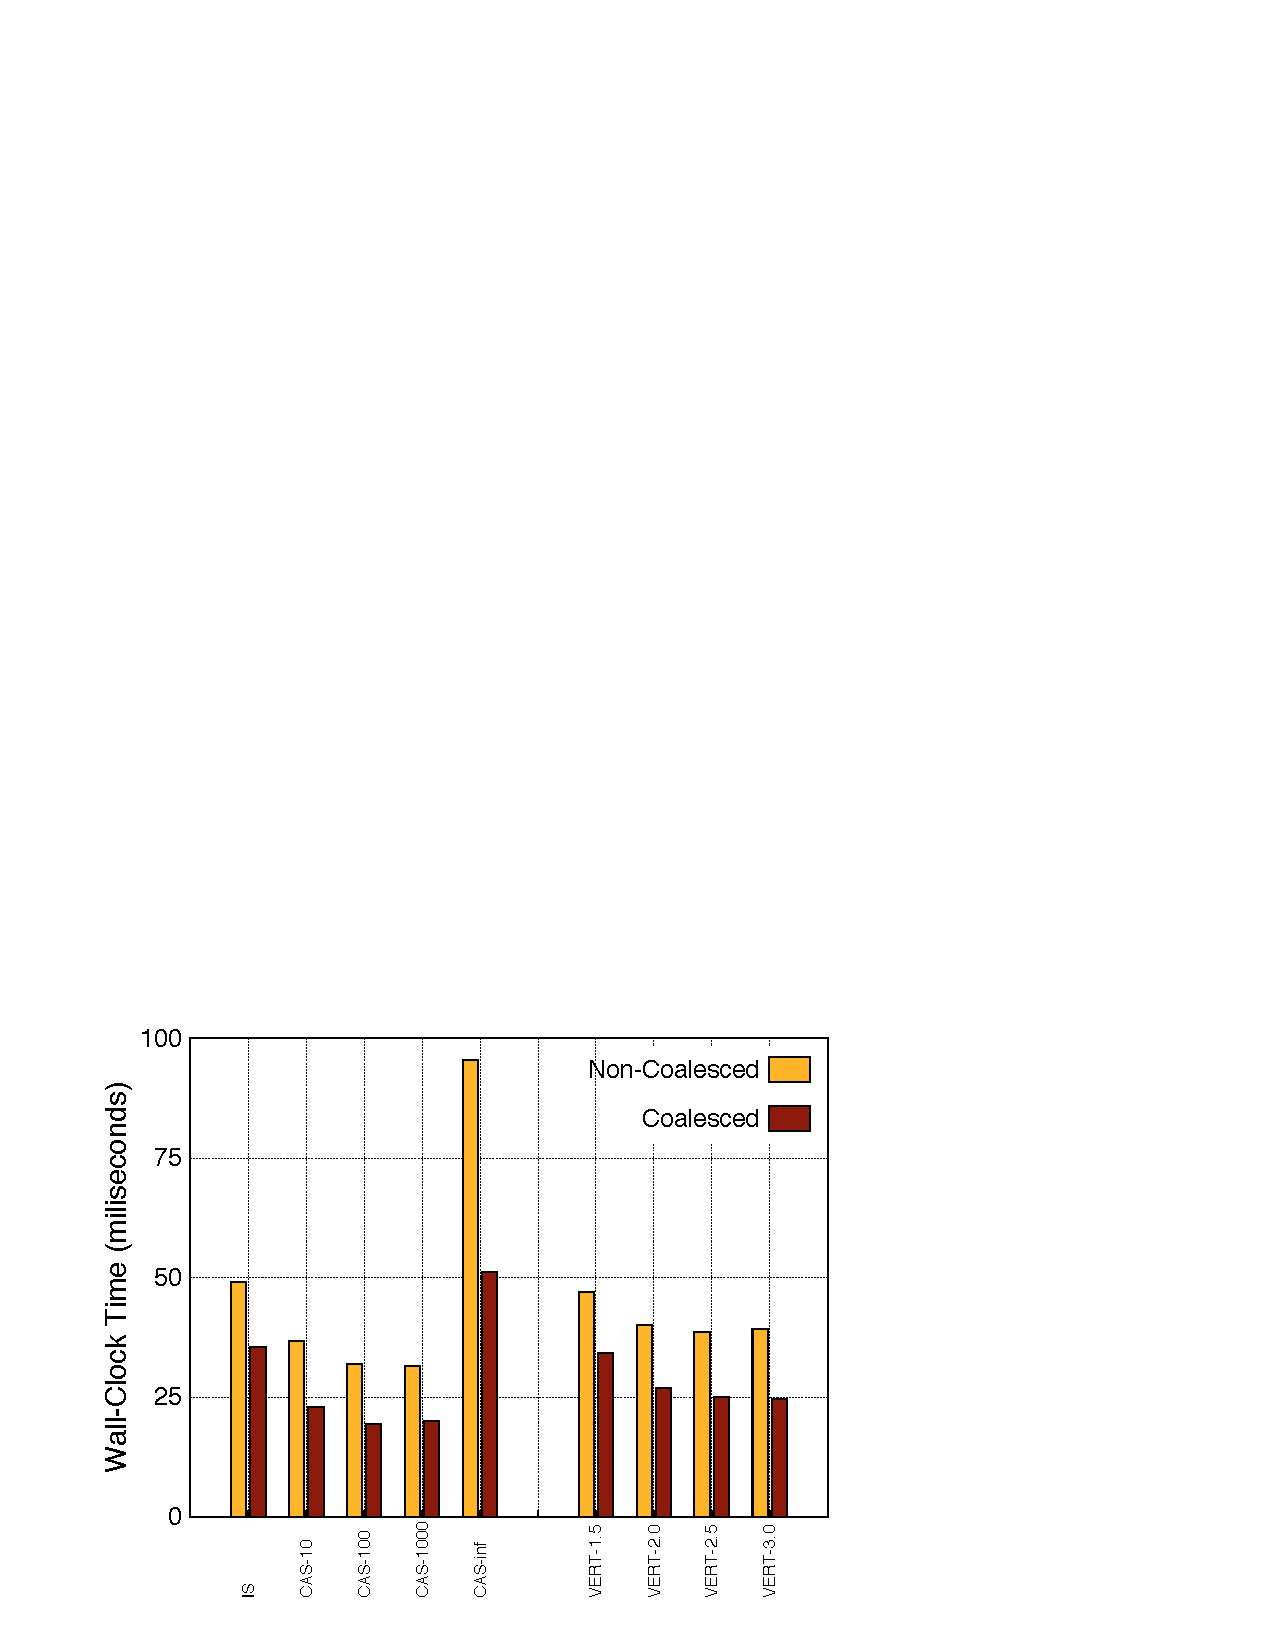
\includegraphics[width=0.5\textwidth]{plots/sharding/monthly-wikipedia.pdf}}
	  \quad
	  \subfigure[UKGOV]{\label{fig:ukgov_query_times_monthly}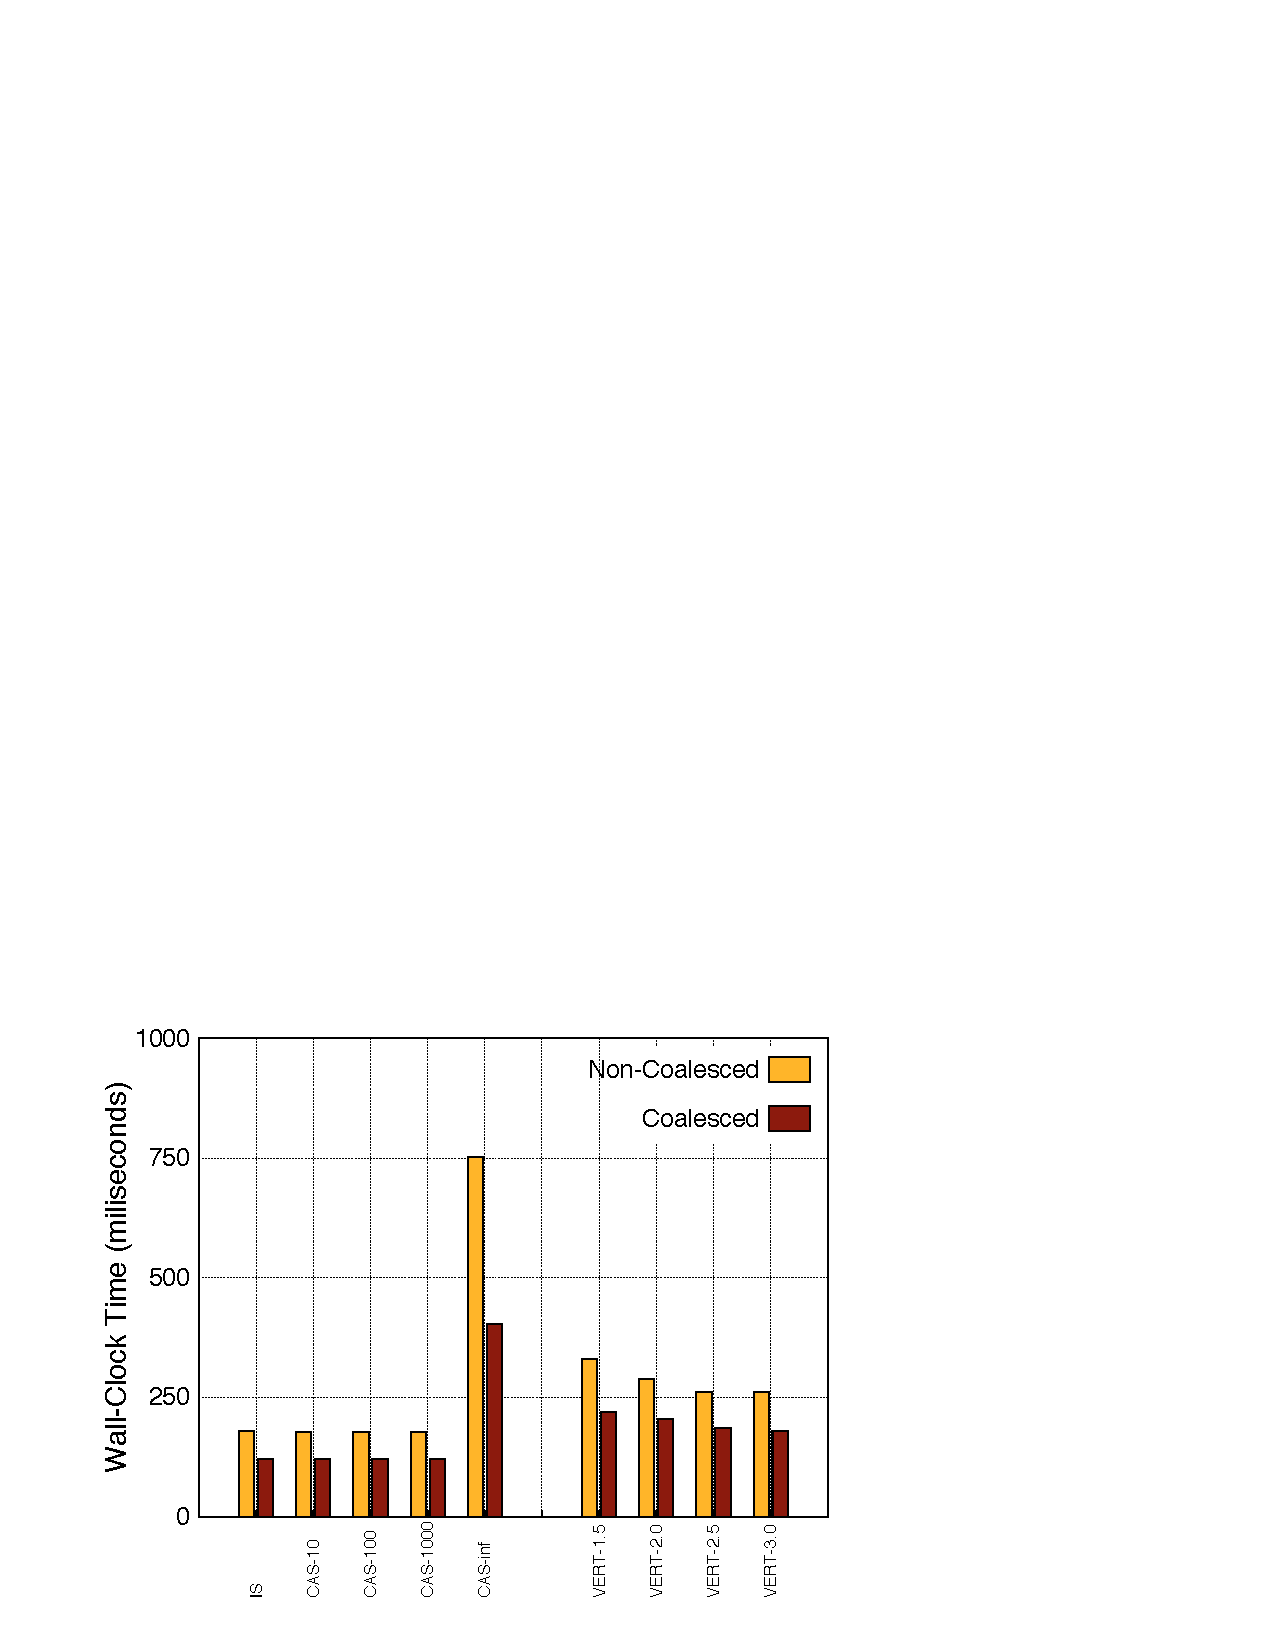
\includegraphics[width=0.5\textwidth]{plots/sharding/monthly-ukgov.pdf}}
   	\caption{Wall-clock times for month-granularity queries}
\label{fig:sharding_qp_cas_vert_month}
\end{figure*}


\subsection{Sharding vs Vertical Partitioning}

In the first set of experiments, we compare the performance of
CAS and VERT on different query granularities. Query granularity of a time-travel text query refers to the time interval component of the query. Figures~\ref{fig:sharding_qp_cas_vert_day} through to~\ref{fig:sharding_qp_cas_vert_full} presents the query response times, in milliseconds, for the different variants of CAS and VERT. Each chart corresponds to the performance of CAS and VERT on a given query granularity -- day (Figure~\ref{fig:sharding_qp_cas_vert_day}), month (Figure~\ref{fig:sharding_qp_cas_vert_month}), year (Figure~\ref{fig:sharding_qp_cas_vert_year}) or the full lifetime of the respective collection (Figure~\ref{fig:sharding_qp_cas_vert_full}). While comparing CAS against VERT, we choose CAS-1000 as a reasonable representative for sharding since the wall-clock times for both CAS-100 and CAS-1000 show low variance throughout all experiments.

%Insight 1: Comparing short time interval queries
VERT-3.0 is optimized for query performance, because of a higher
degree of partitioning, and as expected it has the best performance among its other counterparts ($\kappa = \{1.5, 2.0, 2.5\}$). In case of WIKI, we see a low difference in query
processing times between VERT-3.0 (10.63 ms) and CAS-1000 (11.86 ms) for day-granularity queries (see Figures~\ref{fig:wiki_query_times_daily}). The difference is notable for month-granularity queries with CAS-1000 exhibiting a 19.5\% improvement over VERT-3.0
 (see Figure~\ref{fig:wiki_query_times_monthly}). In UKGOV, CAS-1000 takes
69.88 ms to process day-granularity queries which is almost a 40\% improvement over VERT-3.0 which takes 117.9 ms (see Figure~\ref{fig:ukgov_query_times_daily}). This shows that although VERT is optimized for short time interval queries, and only one or very few partitions have to be accessed for processing, the number of wasted reads accessed in VERT is substantially more those accessed by CAS.

Next, we compare performances for longer time-granularity queries, i.e., year and full-lifetime queries. In
case of WIKI, comparing VERT-1.5, which has the best runtimes for year
queries and lifetime queries, with CAS-1000 shows that the latter
consistently outperforms the former in both cases. Query-processing times improve by
22.2\% (see Figure~\ref{fig:wiki_query_times_yearly}) for year-granularity queries and
by 19\% for full lifetime queries
(see Figure~\ref{fig:wiki_query_times_full}). Note that although VERT-3.0 is optimized to access fewer postings than VERT-1.5, it performs slightly worse. This is possibly because VERT-3.0 has to access more number of partitions than VERT-1.5 for longer time-granularity queries due to its high degree of partitioning. In UKGOV, there is an
improvement of almost 29.9\% or 279.26 ms (CAS-1000 vs
VERT-1.5, see Figure~\ref{fig:ukgov_query_times_yearly}) for year-granularity queries. The full-lifetime queries are faster by 931 ms or 21\% (CAS-1000 vs VERT-1.5, see Figure~\ref{fig:wiki_query_times_full}
and~\ref{fig:ukgov_query_times_full}) which in absolute terms is a considerable difference. Thus, the first insight which we draw is that sharded posting list avoid wasted reads substantially as compared to VERT resulting in superior performance.

%%%Clarify why CAS >>> VERT in terms of number of partitions accessed and wasted reads....build vertical partitions

\begin{figure*}[tb]
	\label{fig:query_times_yearly}	
  	\centering	  
		\subfigure[Wikipedia] {\label{fig:wiki_query_times_yearly} 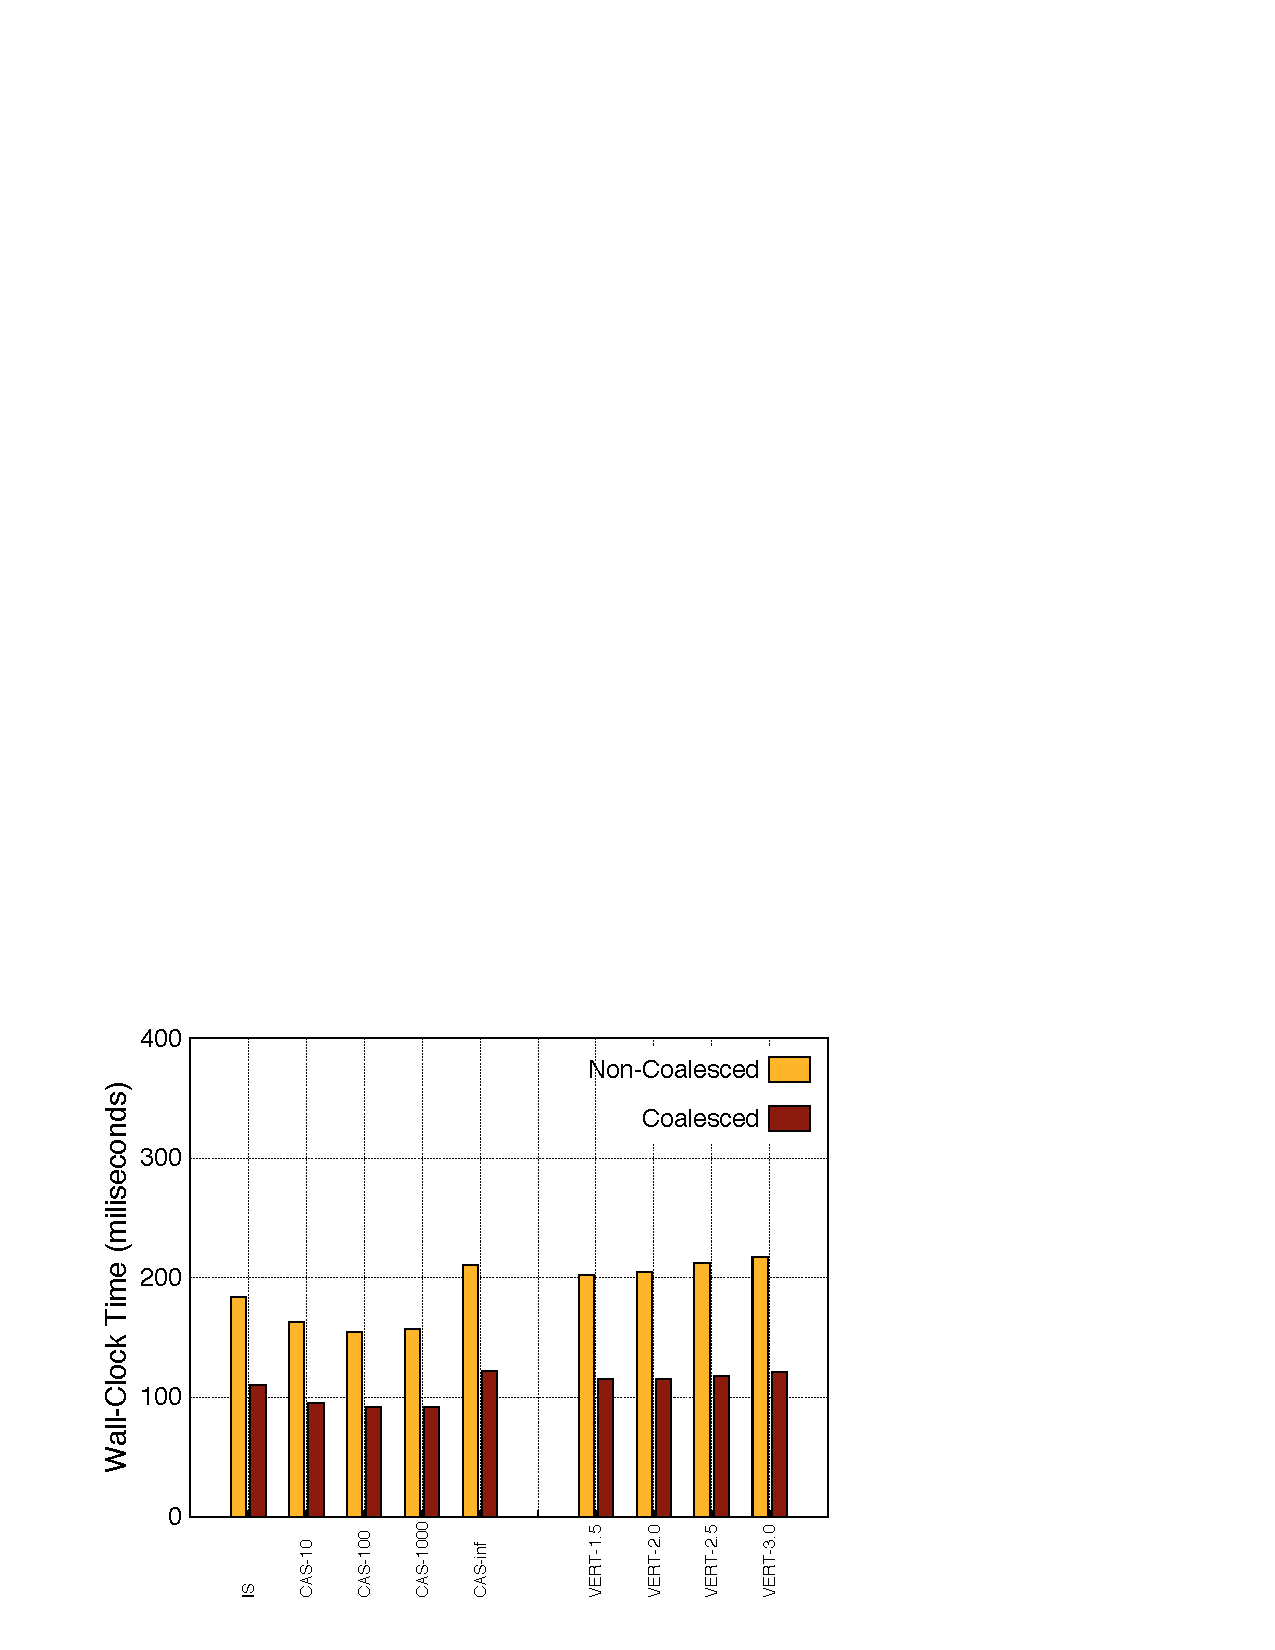
\includegraphics[width=0.5\textwidth]{plots/sharding/yearly-wikipedia.pdf}}
		\quad
		\subfigure[UKGOV]{\label{fig:ukgov_query_times_yearly} 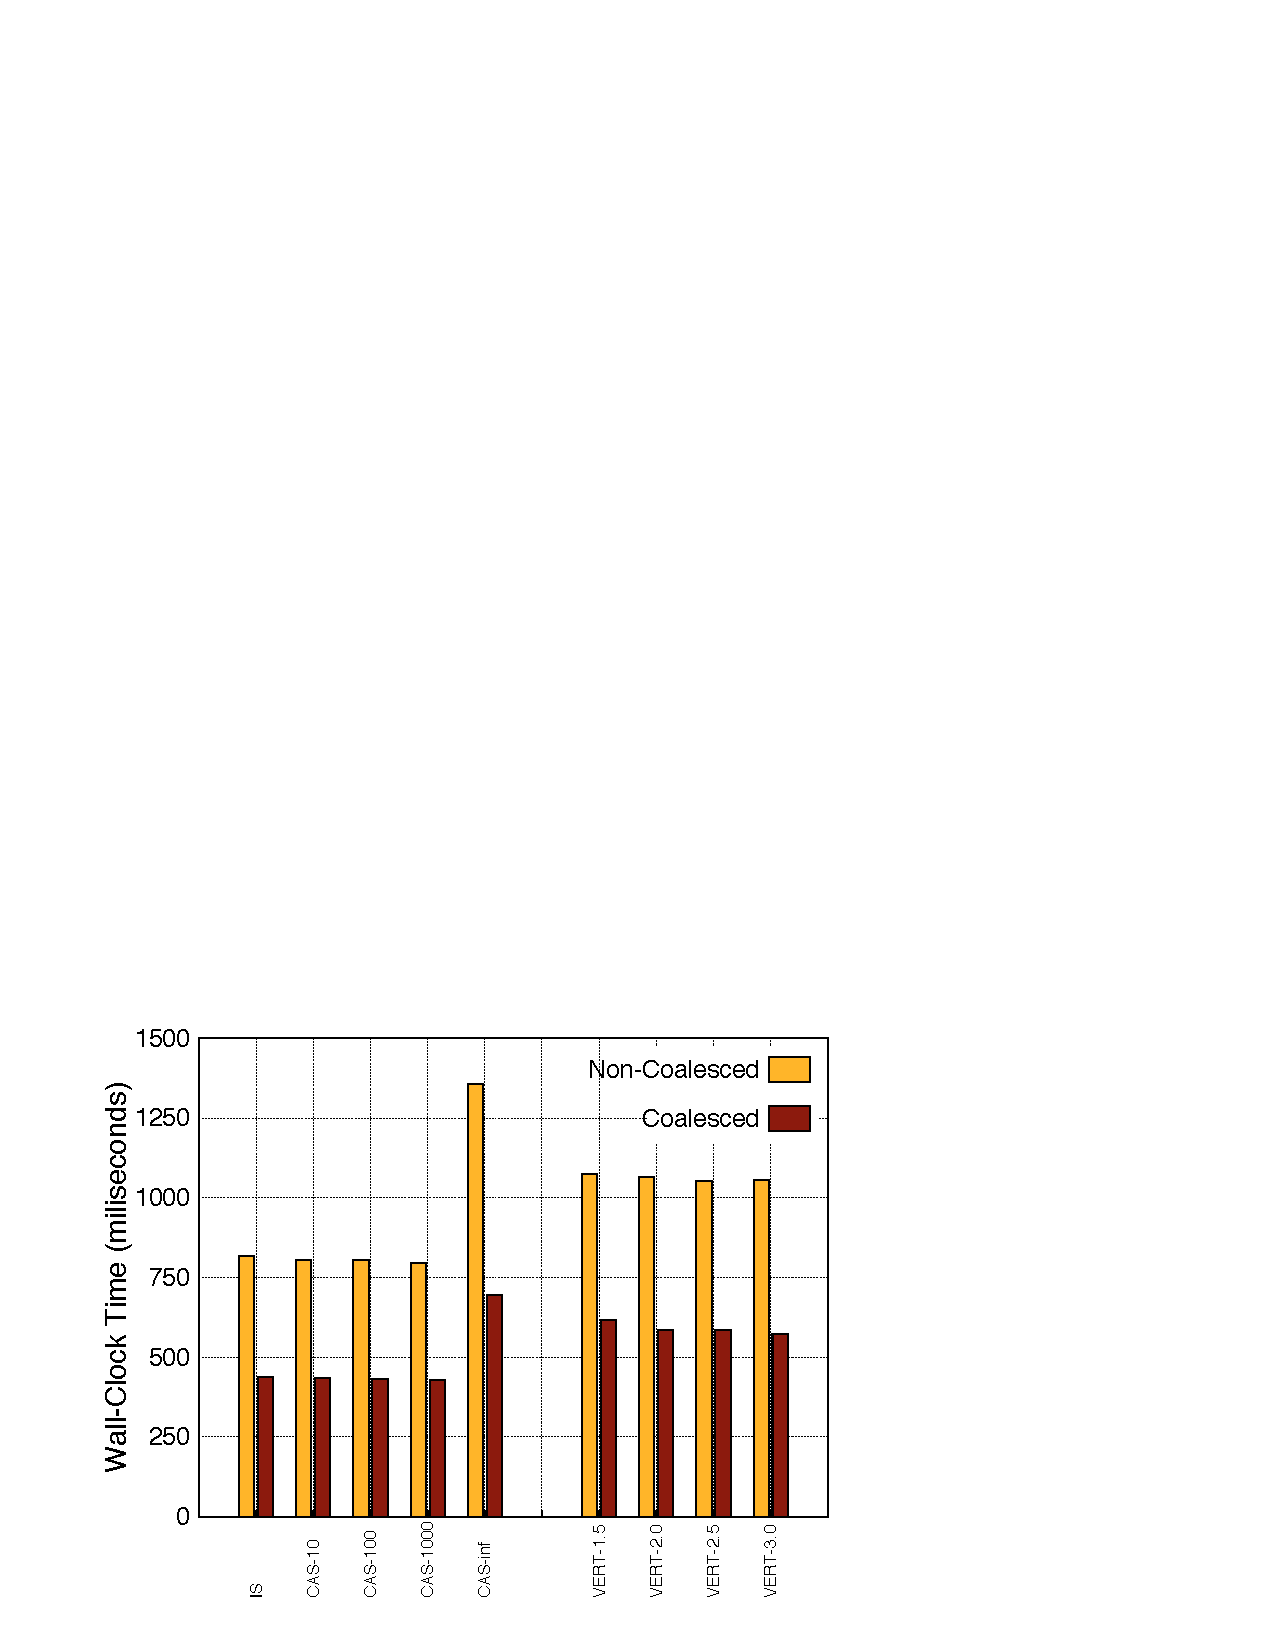
\includegraphics[width=0.5\textwidth]{plots/sharding/yearly-ukgov.pdf}}
   	\caption{Wall-clock times for year-granularity queries}
\label{fig:sharding_qp_cas_vert_year}
\end{figure*}

\begin{figure*}[tb]
  	\centering
	  \subfigure[Wikipedia] {\label{fig:wiki_query_times_full}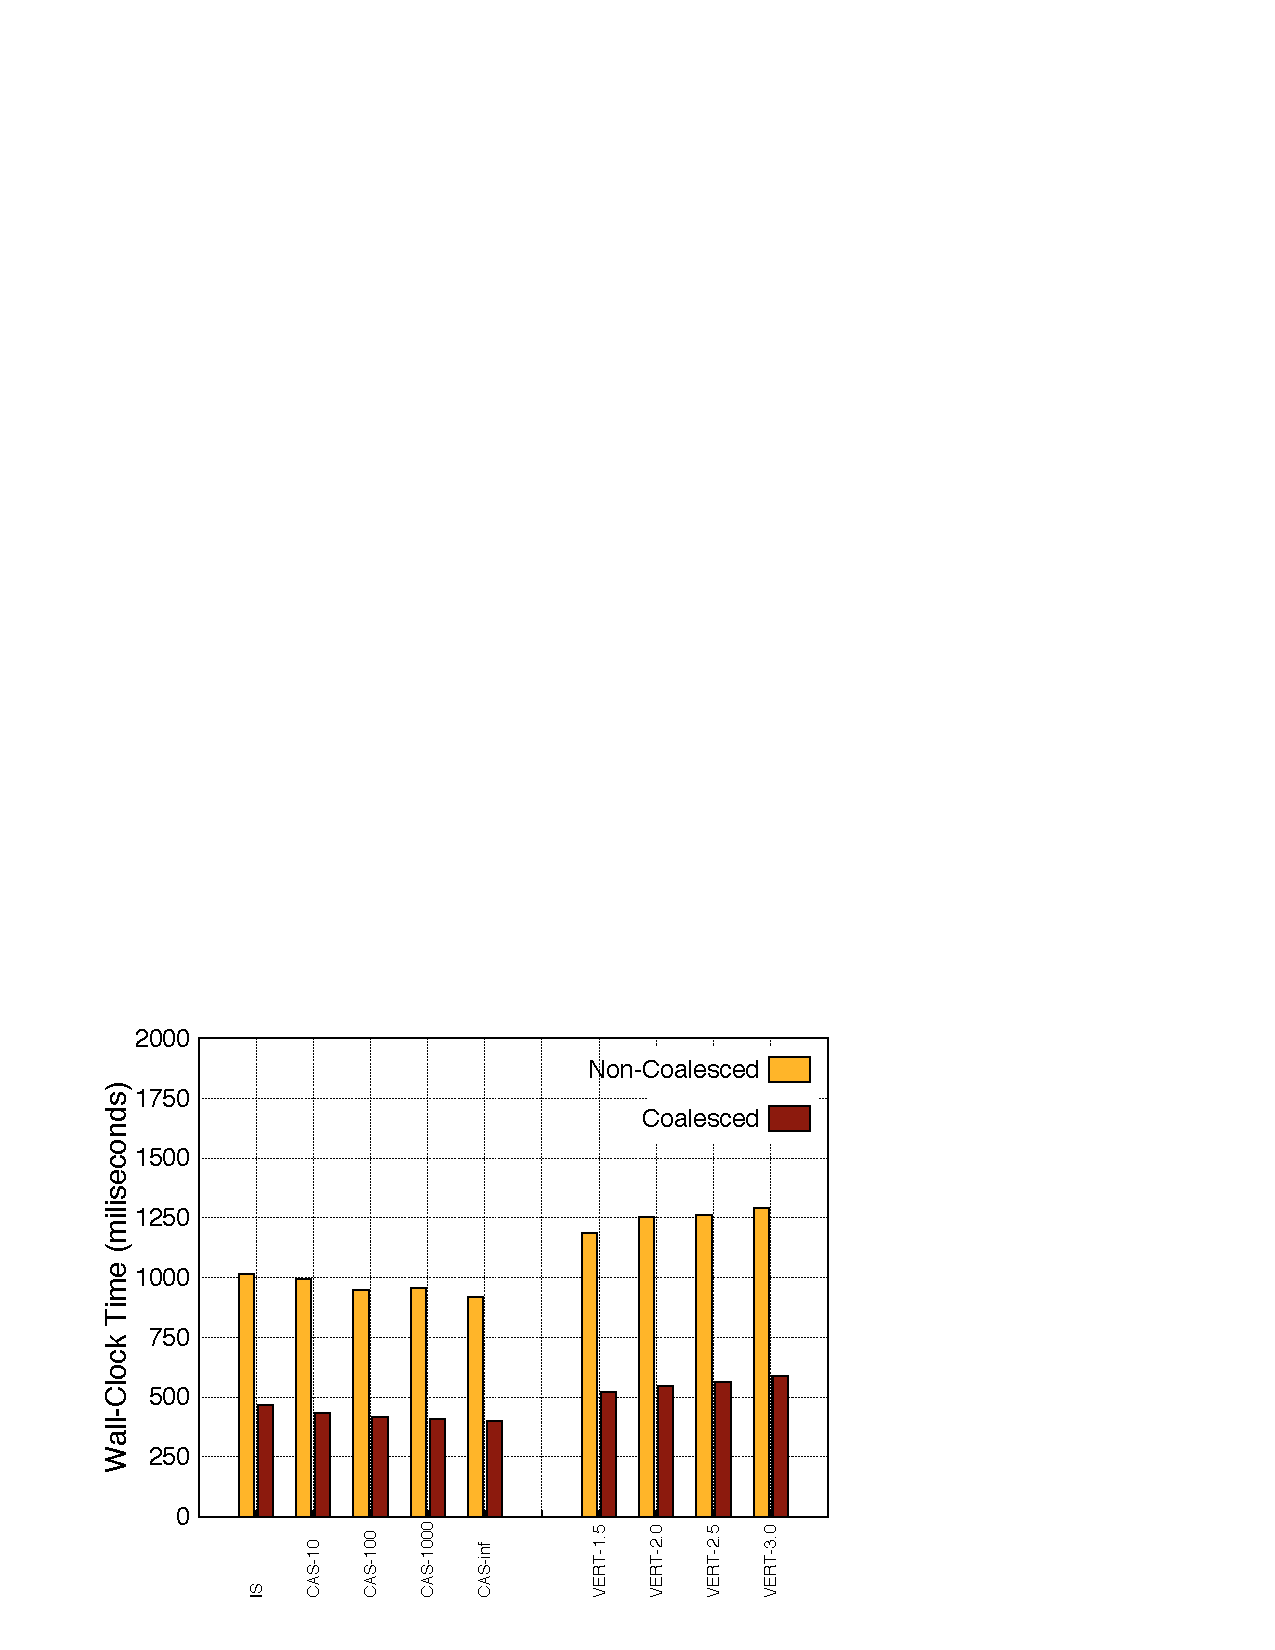
\includegraphics[width=0.5\textwidth]{plots/sharding/full-wikipedia.pdf}}
	  \subfigure[UKGOV] {\label{fig:ukgov_query_times_full} 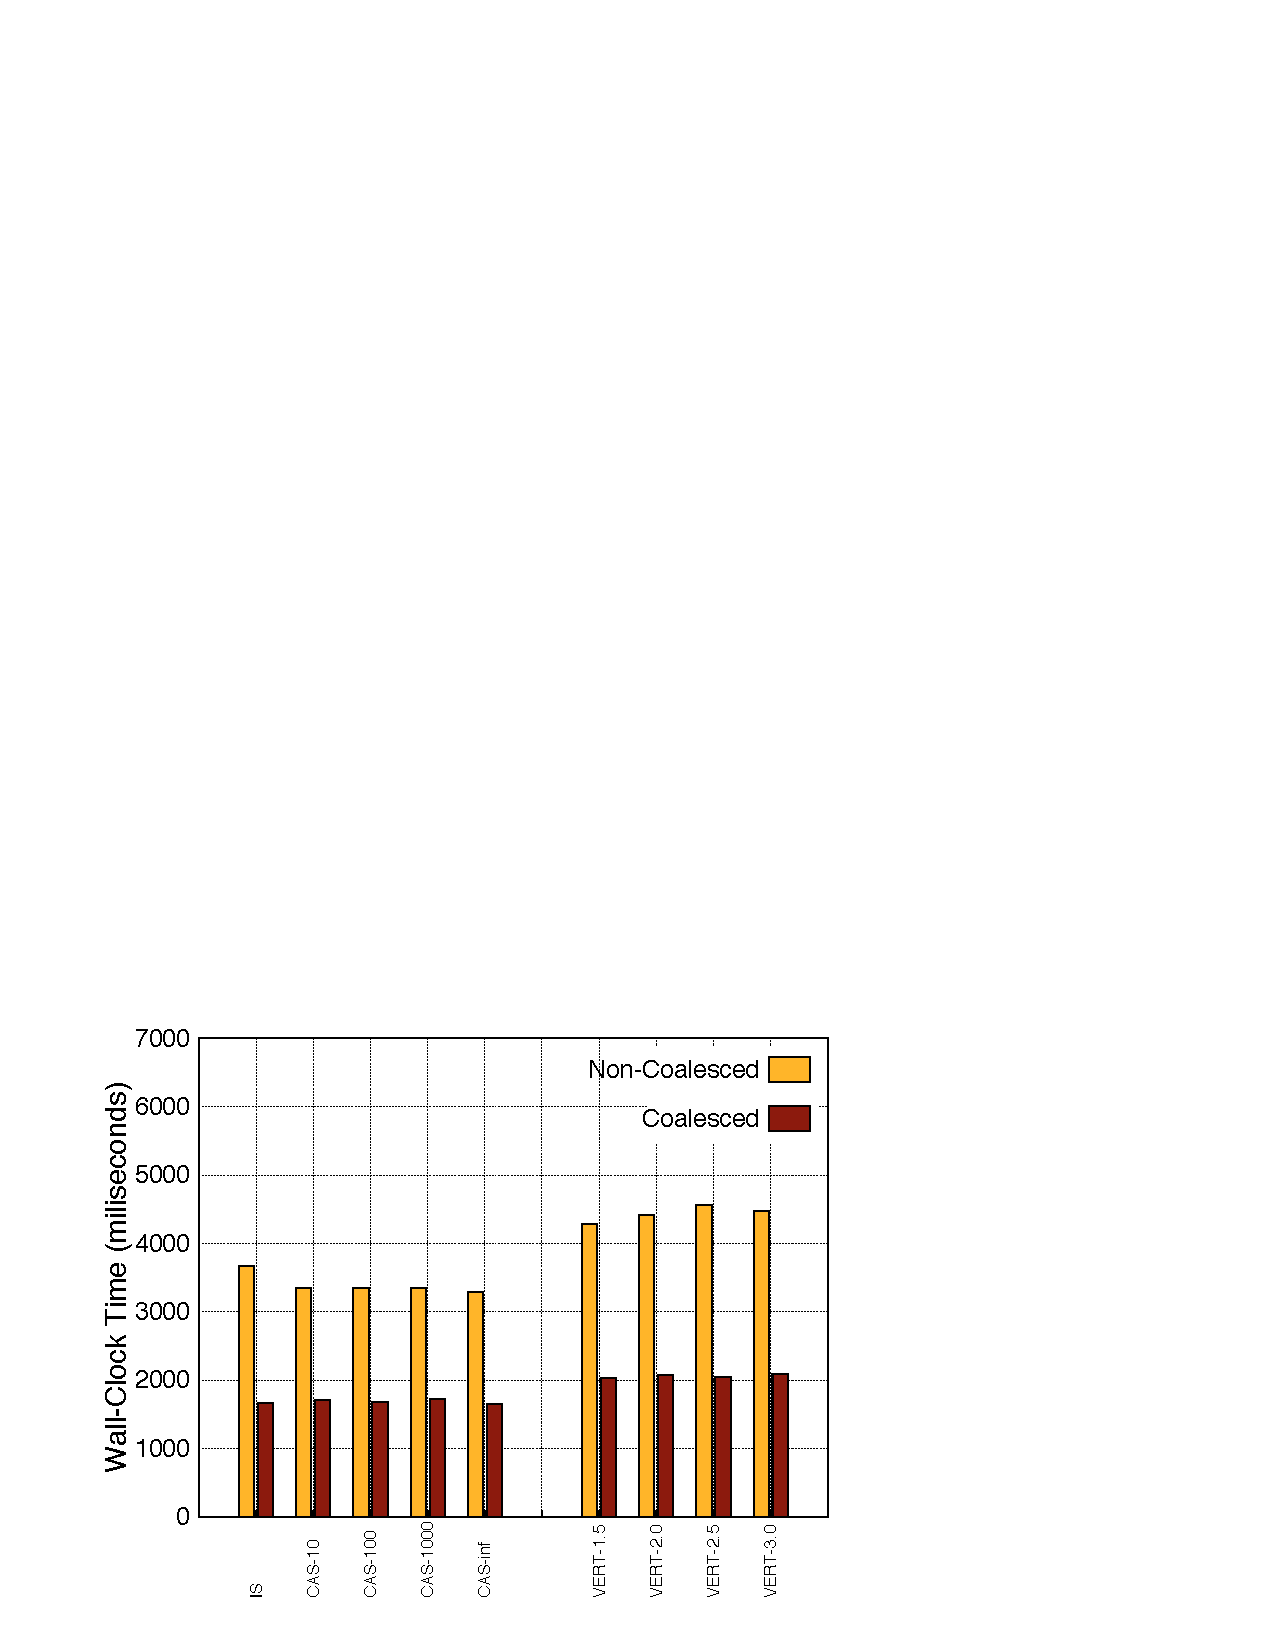
\includegraphics[width=0.5\textwidth]{plots/sharding/full-ukgov.pdf}}
   	\caption{Wall-clock times for full-lifetime queries}
\label{fig:sharding_qp_cas_vert_full}
\end{figure*}

\subsection{Effect of Coalescing}
\label{expt:coa}

Our experimental results with temporal coalescing of postings
lead to similar results as our experiments on the original
uncoalesced indexes. Independent of the partitioning/sharding used,
the index sizes thus obtained are much smaller than with uncoalesced indexes---up to an
order of magnitude for UKGOV and up to a factor of 2 for
Wikipedia. Also the indexes created with sharding are always smaller than
VERT (see Figure~\ref{fig:index_sizes}). The wall-clock times of CAS and VERT methods with temporal coalescing are depicted in
Figures~\ref{fig:wiki_query_times_daily} through~\ref{fig:ukgov_query_times_full}. It is evident that query
performance improves with temporal coalescing, with longer time interval
queries gaining more than those with smaller time ranges as more
postings need to be read. 

\subsection{Comparing Sharding Approaches}

\begin{table}[tb]
  \center
  \begin{tabular}{l @{\hspace{0.2cm}} l @{\hspace{0.3cm}} c @{\hspace{0.3cm}} c}
    \toprule
    & & \multicolumn{2}{c}{\bf Sharding }\\
    \cmidrule{3-4}
    Dataset &$\eta$ & INC & CAS\\
    \midrule
    \multirow{3}{*}{\bf WIKI} 
    & $IS$ & 79.75 & 79.75 \\
    & $10$ & 33.37 & 32.59 \\
    & $100$ & 14.42 & 11.78 \\
    & $1000$ & 6.83 & 4.71 \\
    \\
    \multirow{3}{*}{\bf UKGOV}
    & $IS$ & 16.75 & 16.75 \\
    & $10$ & 11.95 & 14.12 \\
    & $100$ & 8.05 & 11.67 \\
    & $1000$ & 5.49 & 5.84 \\
    \bottomrule
  \end{tabular}
  \caption{Average number of shards per term}
  \label{tab:shard_dist}
\end{table}


\begin{table*}\centering
\begin{tabular}{@{}lrrrrrrrrr@{}}\toprule
& \multicolumn{2}{r}{\textbf{$\eta=10$}} & \phantom{ab} & \multicolumn{2}{r}{\textbf{$\eta=100$}}& \phantom{ab} & \multicolumn{2}{r}{\textbf{$\eta=1000$}}\\ 
\cmidrule{2-3} \cmidrule{5-6} \cmidrule{8-9}
 & CAS & INC && CAS & INC && CAS & INC\\ \midrule
\textbf{WIKI}\\
 Day & 17.64 & 15.81 && 11.57 & 10.65 && 11.86 & 8.70\\
 Month & 29.01 & 28.88 && 25.03 & 24.22 && 24.75 & 22.70\\
 Year & 131.06 & 132.08 && 127.96 & 125.32 && 127.57 & 123.76\\ 
 Full & 851.43 & 817.76 && 834.74 & 806.87 && 815.20 & 809.90\\
 %\textbf{Overall} & - & 51 && 65 & - && - & -\\
\midrule
\textbf{UKGOV}\\
 Day  & 55.78 & 50.22 && 53.34 & 44.97 && 49.25 & 43.27\\
 Month & 158.89 & 155.72 && 156.28 & 145.77 && 153.89 & 143.60\\
 Year  & 711.63 & 724.56 && 707.84 & 702.69 && 699.81 & 696.87 \\ 
 Full  & 2,875.35 & 2,839.80 && 2,794.46 & 2,845.31 && 2,940.5 & 2,999.32 \\
 %\textbf{Overall} & - & 51 && 65 & - && - & -\\
 \bottomrule
\end{tabular}
\caption{Comparison of wall-clock times between CAS and INC -- in milliseconds}

\label{tab:sharding_qp}
\end{table*}

In the next set of results, we first present the improvements, in query-processing wall-clock times, due to reductions in the number of shards by carefully allowing for wasted reads regulated by the parameter $\eta$. Secondly, we compare the query performance of both sharding approaches CAS and INC. 

To explain the query performance of the sharding methods, we first compare the average number of shards generated by both the algorithms for the terms present in the query workload. These results are summarized in Table~\ref{tab:shard_dist}. Interestingly, INC has lesser number of shards than CAS in UKGOV in-spite of being more restrictive. This means that the INC, with an approximation guarantee, seems to make better choices than the heuristic approach employed by CAS. On the contrary for WIKI the number of shards per term created by INC is more than that of CAS. However, in both these cases the difference between CAS and INC in the number of shards is not significant.

\paragraph{Effect of the Parameter $\eta$}  Depending on the value of the parameter $\eta$ there are two conceptual extremes in sharding. The scenario $\eta = 0$ represents idealized sharding, denoted by IS, when wasted reads are completely avoided. Note that both CAS and INC would give rise to IS when $\eta = 0$. The other extreme is CAS-inf which results in no sharding of the posting list. cop 

Idealized sharding is a restrictive form of sharding and for certain distributions produces a fairly high number of shards (see Table~\ref{tab:shard_dist}). Although query processing on IS results in reading only the postings intersecting with the query time-interval, they suffer
from inefficiencies due to a large number of random seeks in accessing each shard individually. Especially
for disk with $C_r >> C_s$, the open-seek operation on idealized
shards might result in considerable overheads. 

To put this into perspective with the actual query performance, we present the wall-clock times in Table~\ref{tab:sharding_qp}. In WIKI, we see a consistent improvement from IS to CAS-1000. This is
because idealized sharding admits a fairly large number of shards in
this case and thus the I/O costs are dominated by initial random seeks
to access these idealized shards. Improvements result from the
reduction in the number of shards due to careful merging of idealized
shards, as presented before in Section~\ref{chap:sharding:sec:relaxed_part}. Although
these reductions might not be significant for queries with longer
time intervals, but they reduce query processing time by a sizable
fraction for small-time granularity queries -- day-granularity queries improve by
62\% (see Figure~\ref{fig:wiki_query_times_daily}) and month-granularity queries by
35\% (see Figure~\ref{fig:wiki_query_times_monthly}). A similar trend is seen in the case of INC (see Table~\ref{tab:sharding_qp}) where there is a 47\% improvement in day-granularity queries in INC-1000 from INC-10 for WIKI. Unlike WIKI, the  difference in performance between CAS and INC in UKGOV is not considerable, which is due
to the already low number of initial idealized shards. This indicates
that sharding can be applied as a self-organizing approach
depending on the distribution of initial shards. 

CAS-1000, and eventually INC-1000, outperforms CAS-inf by a fairly large margin in all
query granularities except one scenario. This shows that the improvement in query performance is not only due to begin-time order of postings in the shards but a result of careful sharding of posting lists to avoid wasted reads. The only scenario when CAS-inf outperforms others is when we consider queries spanning the full-lifetime of the collection. This behavior is to be expected because all postings in CAS-inf
become relevant for such kind of queries and have to be subsequently
read. 

 
\paragraph{Comparing CAS and INC}  As one can observe from the in Table~\ref{tab:sharding_qp}, the sharded index generated using INC compares quite favourably with the CAS. This behaviour is consistent across all the granularities of temporal predicates for all values of $\eta$. In a small number of cases, the performance of INC is slightly better than that of CAS, and is never worse. Although we see a less shards in some scenarios, it is counteracted more number of wasted reads per shard for a given query. Hence, the small differences in the number of shards between CAS and INC do not to make a considerable difference in the wall-clock times. Hence the arguments presented above comparing CAS and VERT also apply when comparing INC and VERT.

% \aanand{reformulate....}
% So, when the underlying storage system has high cost of
% random accesses, then it seems more beneficial to query processing
% performance to use INC to maintain the index than using CA. 

\subsection{Index Sizes}


\begin{figure*}[tp]
  	\centering	
	  	\subfigure[Wikipedia] {\label{fig:wiki_idx_sizes}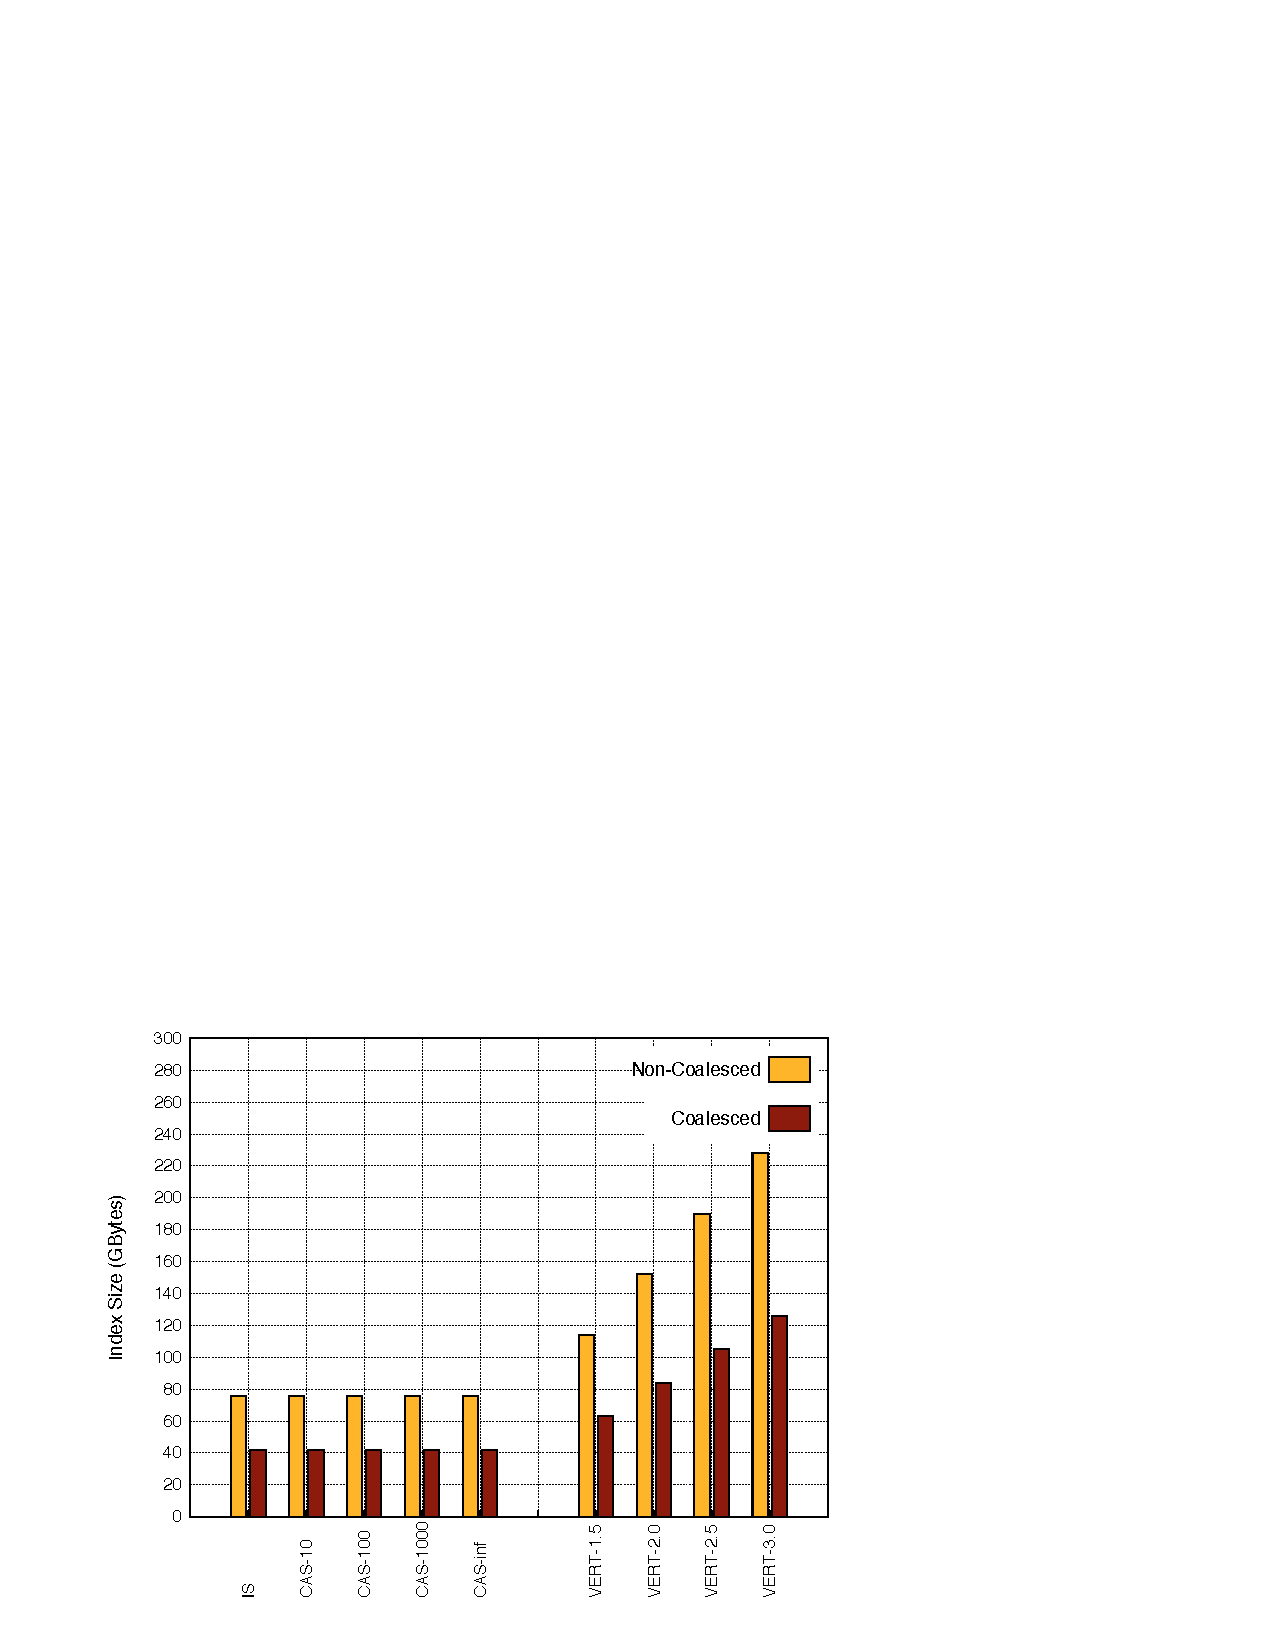
\includegraphics[width=0.4\textwidth]{plots/sharding/index-sizes-wikipedia.pdf}}
		\quad
		\subfigure[UKGOV]{\label{fig:ukgov_idx_sizes}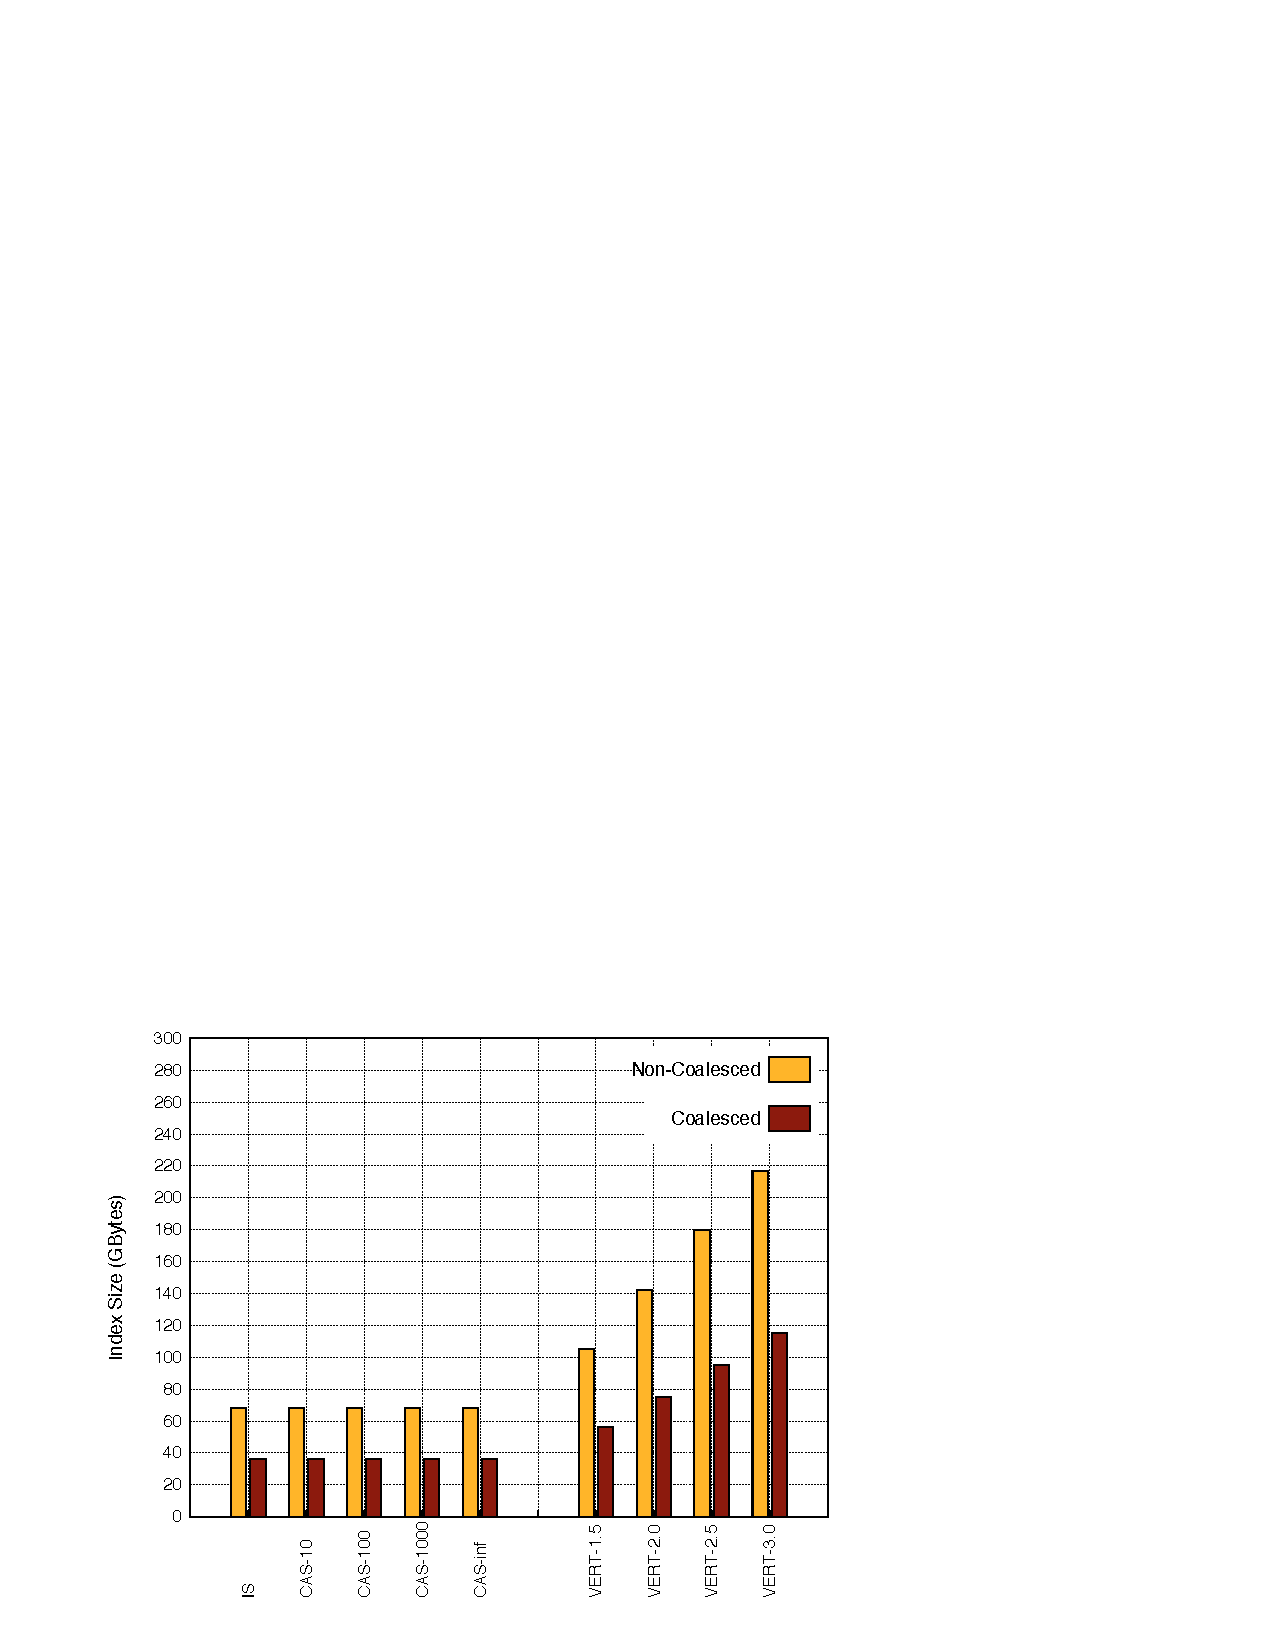
\includegraphics[width=0.4\textwidth]{plots/sharding/index-sizes-ukgov.pdf}}
   	\caption{Index sizes}
   	\label{fig:index_sizes}
\end{figure*}


\begin{table*}\centering
\begin{tabular}{@{}lrrrrrrrrr@{}}\toprule
& \multicolumn{2}{c}{\textbf{$\eta=10$}} & \phantom{ab} & \multicolumn{2}{c}{\textbf{$\eta=100$}}& \phantom{ab} & \multicolumn{2}{c}{\textbf{$\eta=1000$}}\\ 
\cmidrule{2-3} \cmidrule{5-6} \cmidrule{8-9}
 & CAS & INC && CAS & INC && CAS & INC\\ \midrule
\textbf{WIKI} & 76.31 & 78.50 && 76.29 & 77.60 && 76.18 & 77.20\\
\textbf{UKGOV} & 68.31 & 68.50 && 68.28 & 68.47 && 68.18 & 68.46\\
 \bottomrule
\end{tabular}
\caption{Comparison between index sizes of CAS and INC - in gigabytes}

\label{tab:sharding_idx_sizes}
\end{table*}

As expected, the size of the index files of the sharded indexes is the same as that of the unpartitioned index. This is due to the fact
that sharding partitions the postings of the unpartitioned lists in a
disjoint manner. On the contrary the postings in VERT are
subject to replication across the vertical partitions. The index sizes of the different variants of VERT show a direct correlation with the input
parameter $\kappa$ as shown in Figure ~\ref{fig:wiki_idx_sizes}. As
discussed before, $\kappa$ regulates the upper bound to the index-size
blowup. The higher the $\kappa$, the more efficient is the performance
of time-travel queries at the expense of a larger index
size.  Thus the vertically-partitioned index has to be carefully tuned trading off index size and query
efficiency. This is not the case with the sharded index where the
tradeoff is between number of random seeks and sequential reads, which
are local tunable parameters depending on physical characteristics of
disks (where the index is stored) irrespective of the query
workload. 

The difference in overall index sizes is due to the impact lists. Since each shard is associated with an impact list, the number of shards in an index is directly correlated with size of the impact-list file. Thus, the file which store the impact lists decrease with the increasing $\eta$. Each impact list is stored as list of pairs of integers without compression. From our experiments we see that the impact-list file is typically 1\%-7\% of the entire index. There is, however, scope for compactly representing the impact lists using integer compression over d-gaps when the key and values are stored in integer array separately. 

%We did not explore them in this set of experiments. 

From our experiments, we observe that the time taken to build
a sharded index is roughly twice the time taken for the standard
unpartitioned inverted index. Since the sharded index building process
can be easily parallelized, one can efficiently build sharded indexes
using a distributed processing platform (e.g., Hadoop).


\begin{figure*}[]
  \centering \subfigure[$\eta$ =
  10]{\label{fig:wiki_index_merge_10.0}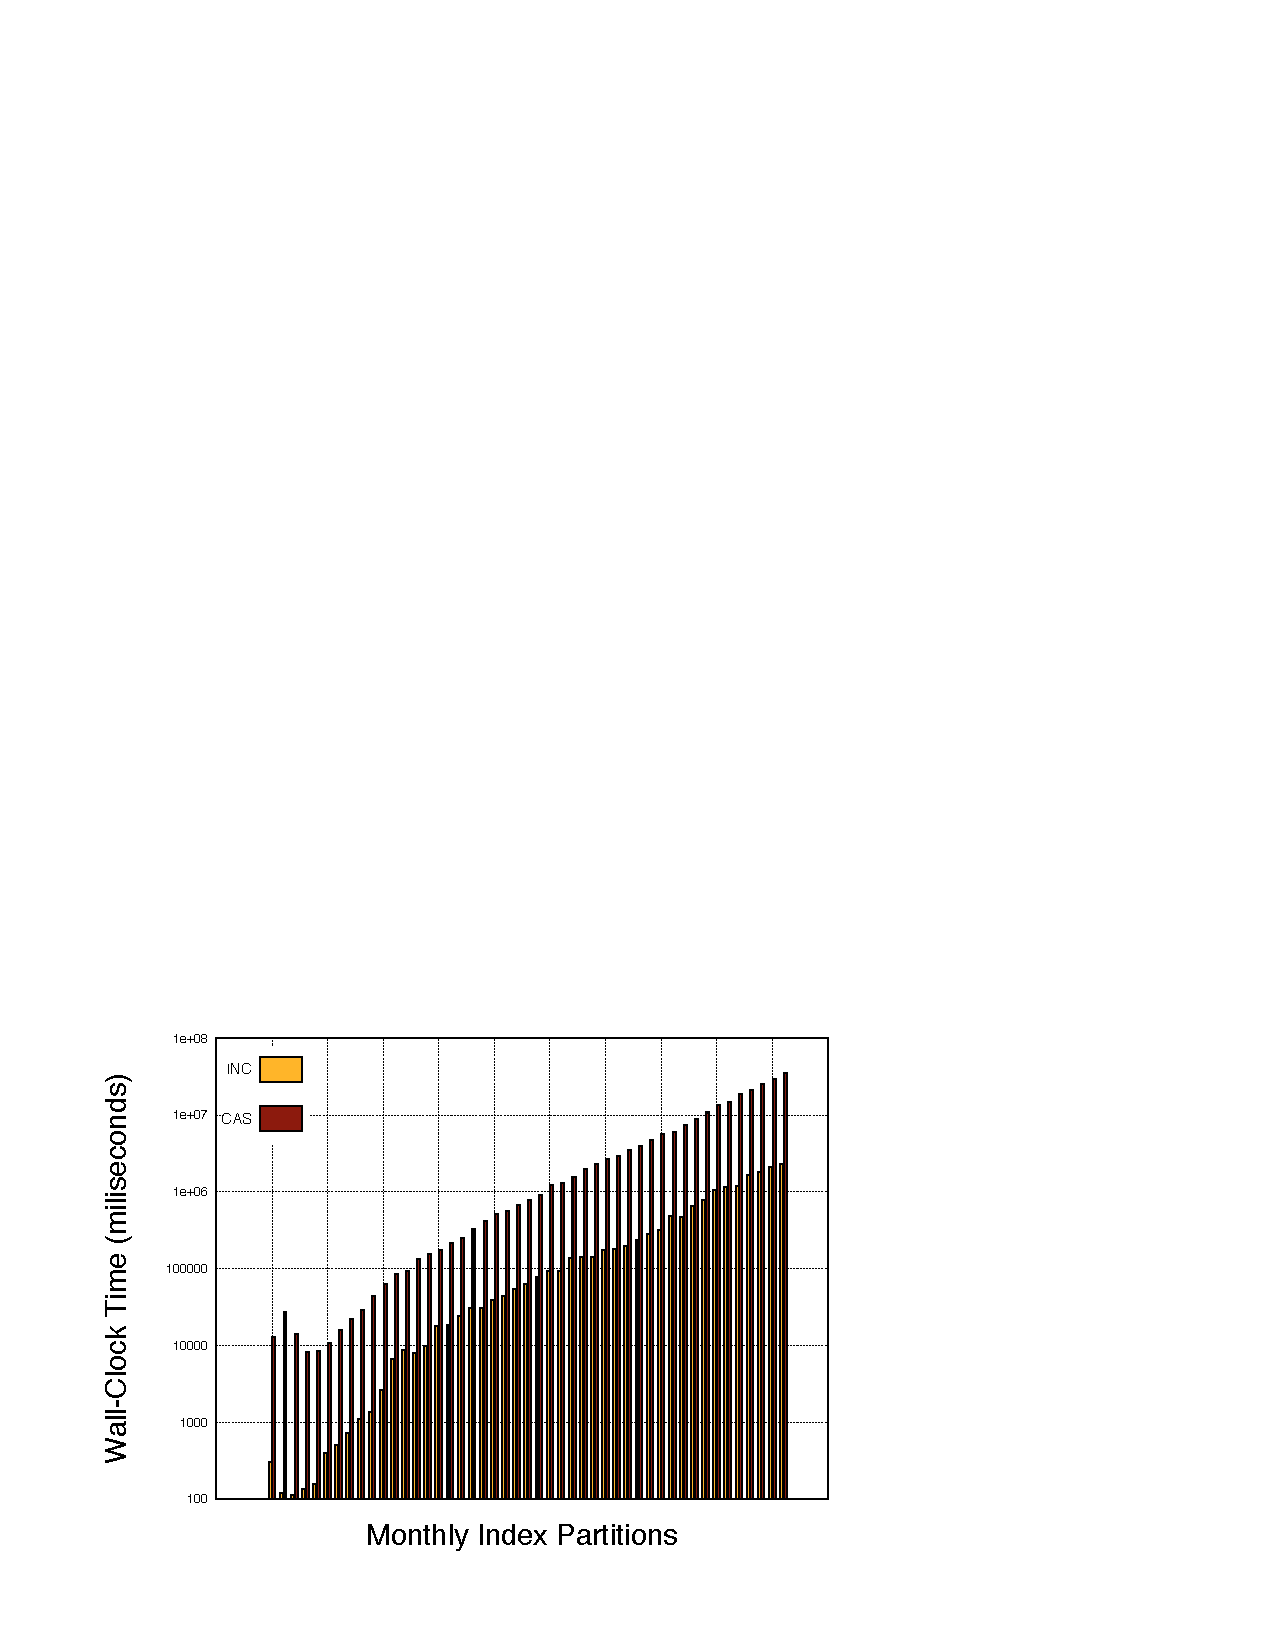
\includegraphics[width=0.6\textwidth]{plots/updates/pdfs/index_maintenance_wiki_10.pdf}}
  %\quad
  \subfigure[$\eta$ =
  100]{\label{fig:wiki_index_merge_100.0}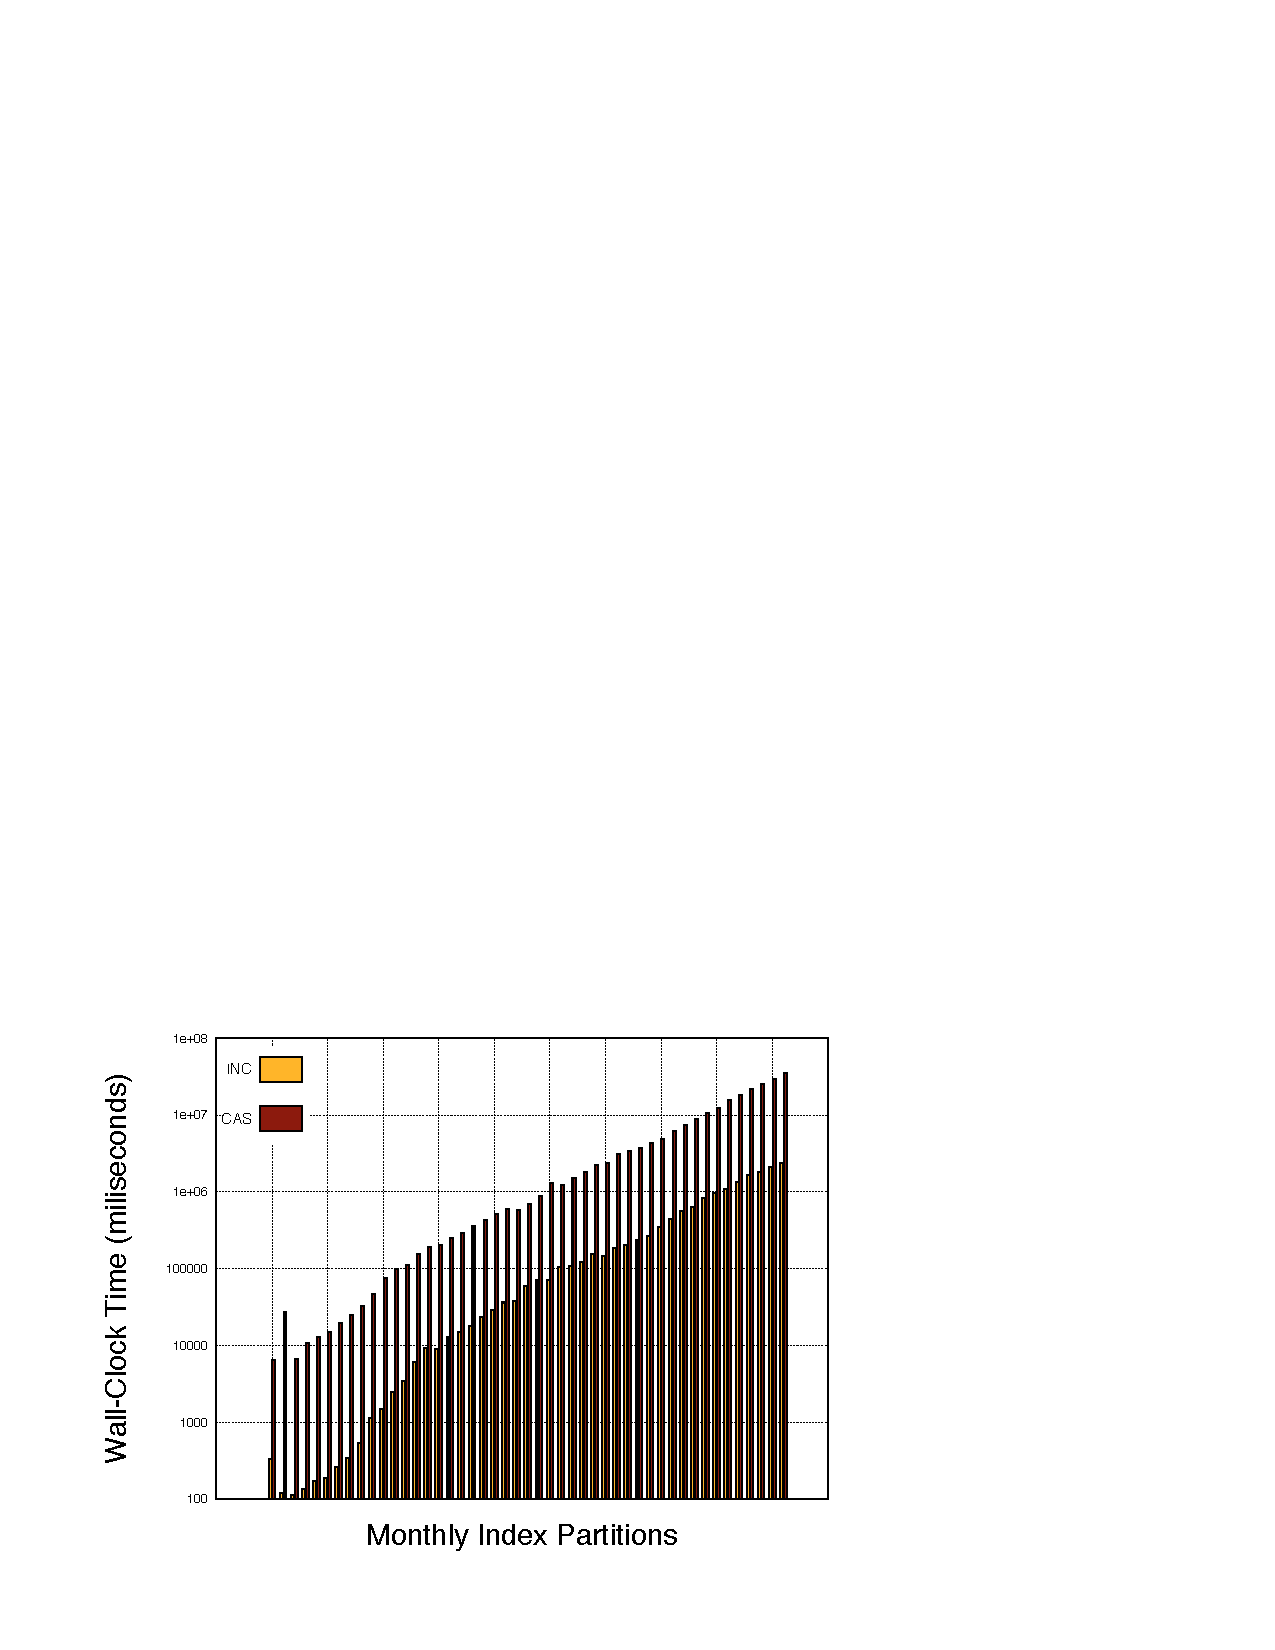
\includegraphics[width=0.6\textwidth]{plots/updates/pdfs/index_maintenance_wiki_100.pdf}}
  \quad
  \subfigure[$\eta$ =
  1000]{\label{fig:wiki_index_merge_1000.0}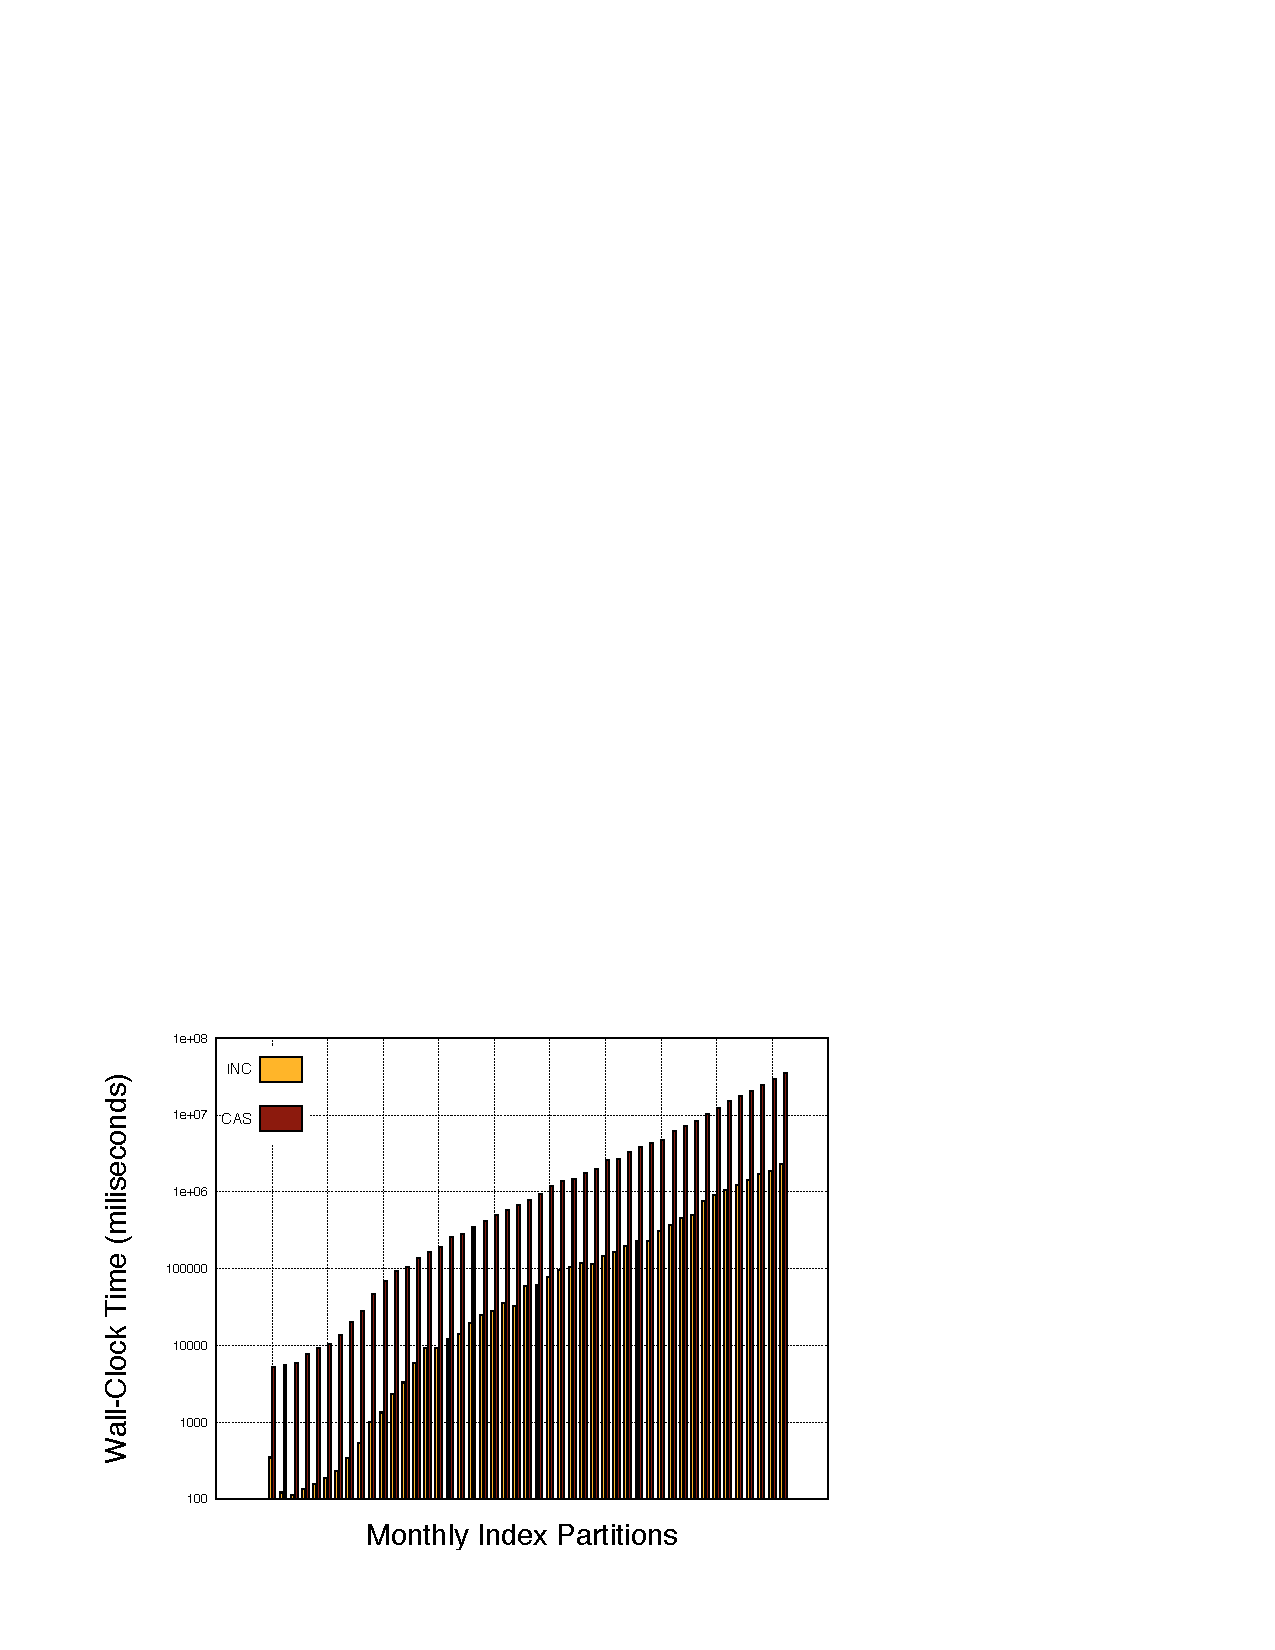
\includegraphics[width=0.6\textwidth]{plots/updates/pdfs/index_maintenance_wiki_1000.pdf}}
  \caption{Performance of index maintenance - WIKI}
  \label{fig:imwiki}
\end{figure*}


\begin{figure*}[]
  \centering \subfigure[$\eta$ =
  10]{\label{fig:ukgov_index_merge_10.0}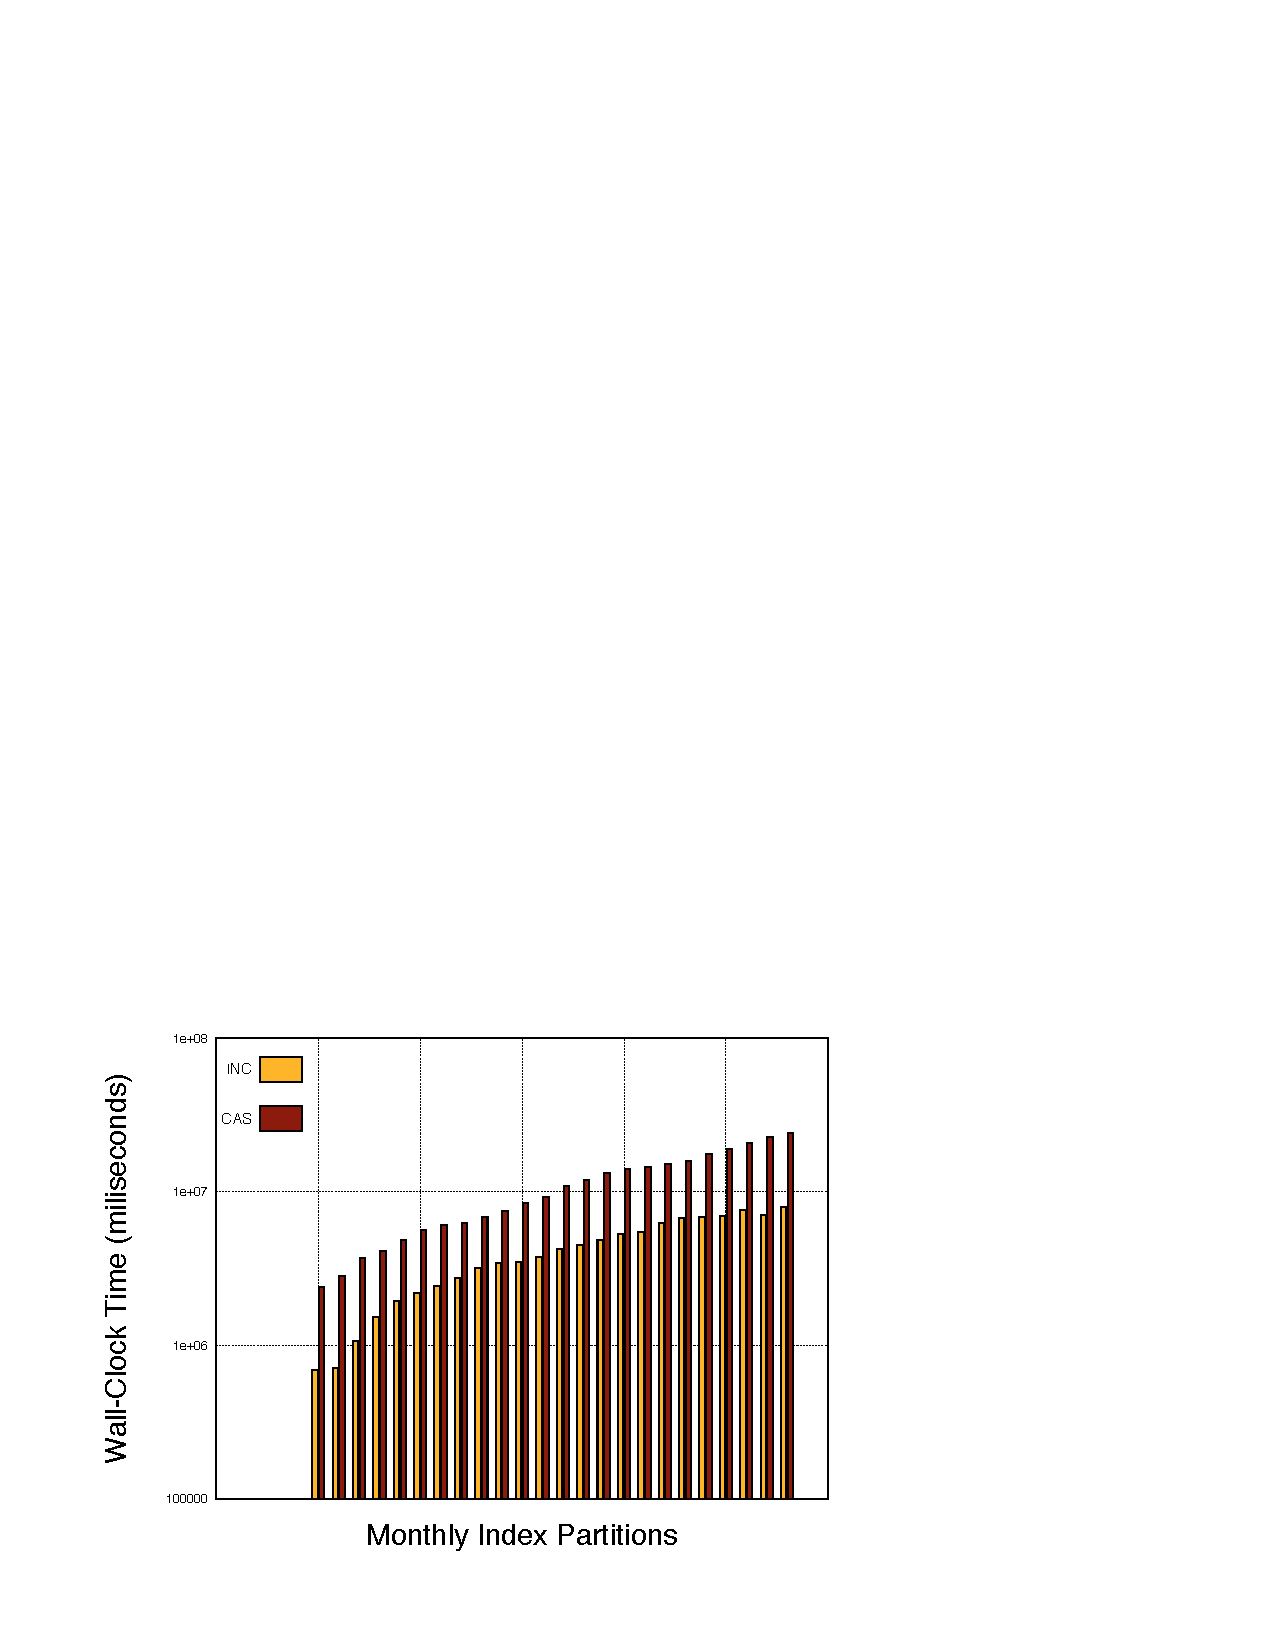
\includegraphics[width=0.6\textwidth]{plots/updates/pdfs/index_maintenance_ukgov_10.pdf}}
  %\quad
  \subfigure[$\eta$ =
  100]{\label{fig:ukgov_index_merge_100.0}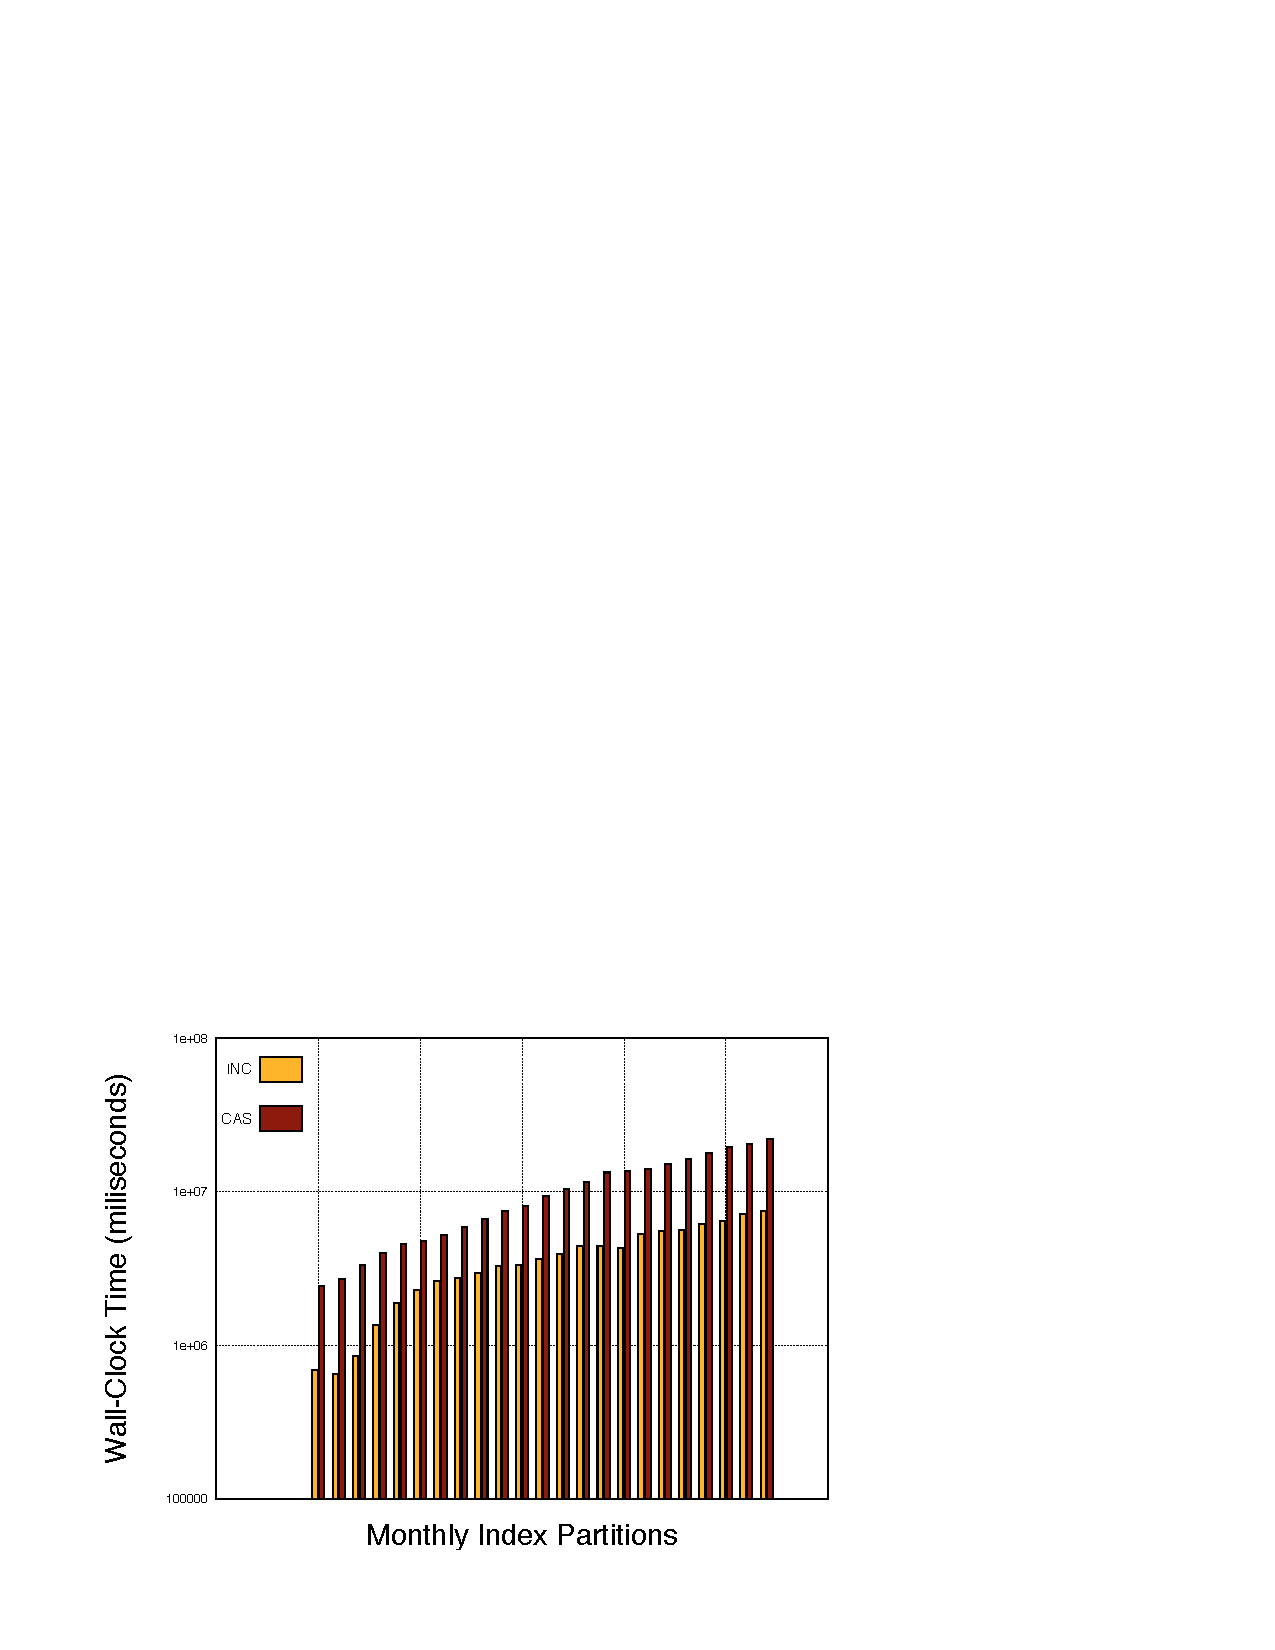
\includegraphics[width=0.6\textwidth]{plots/updates/pdfs/index_maintenance_ukgov_100.pdf}}
  \quad
  \subfigure[$\eta$ =
  1000]{\label{fig:ukgov_index_merge_1000.0}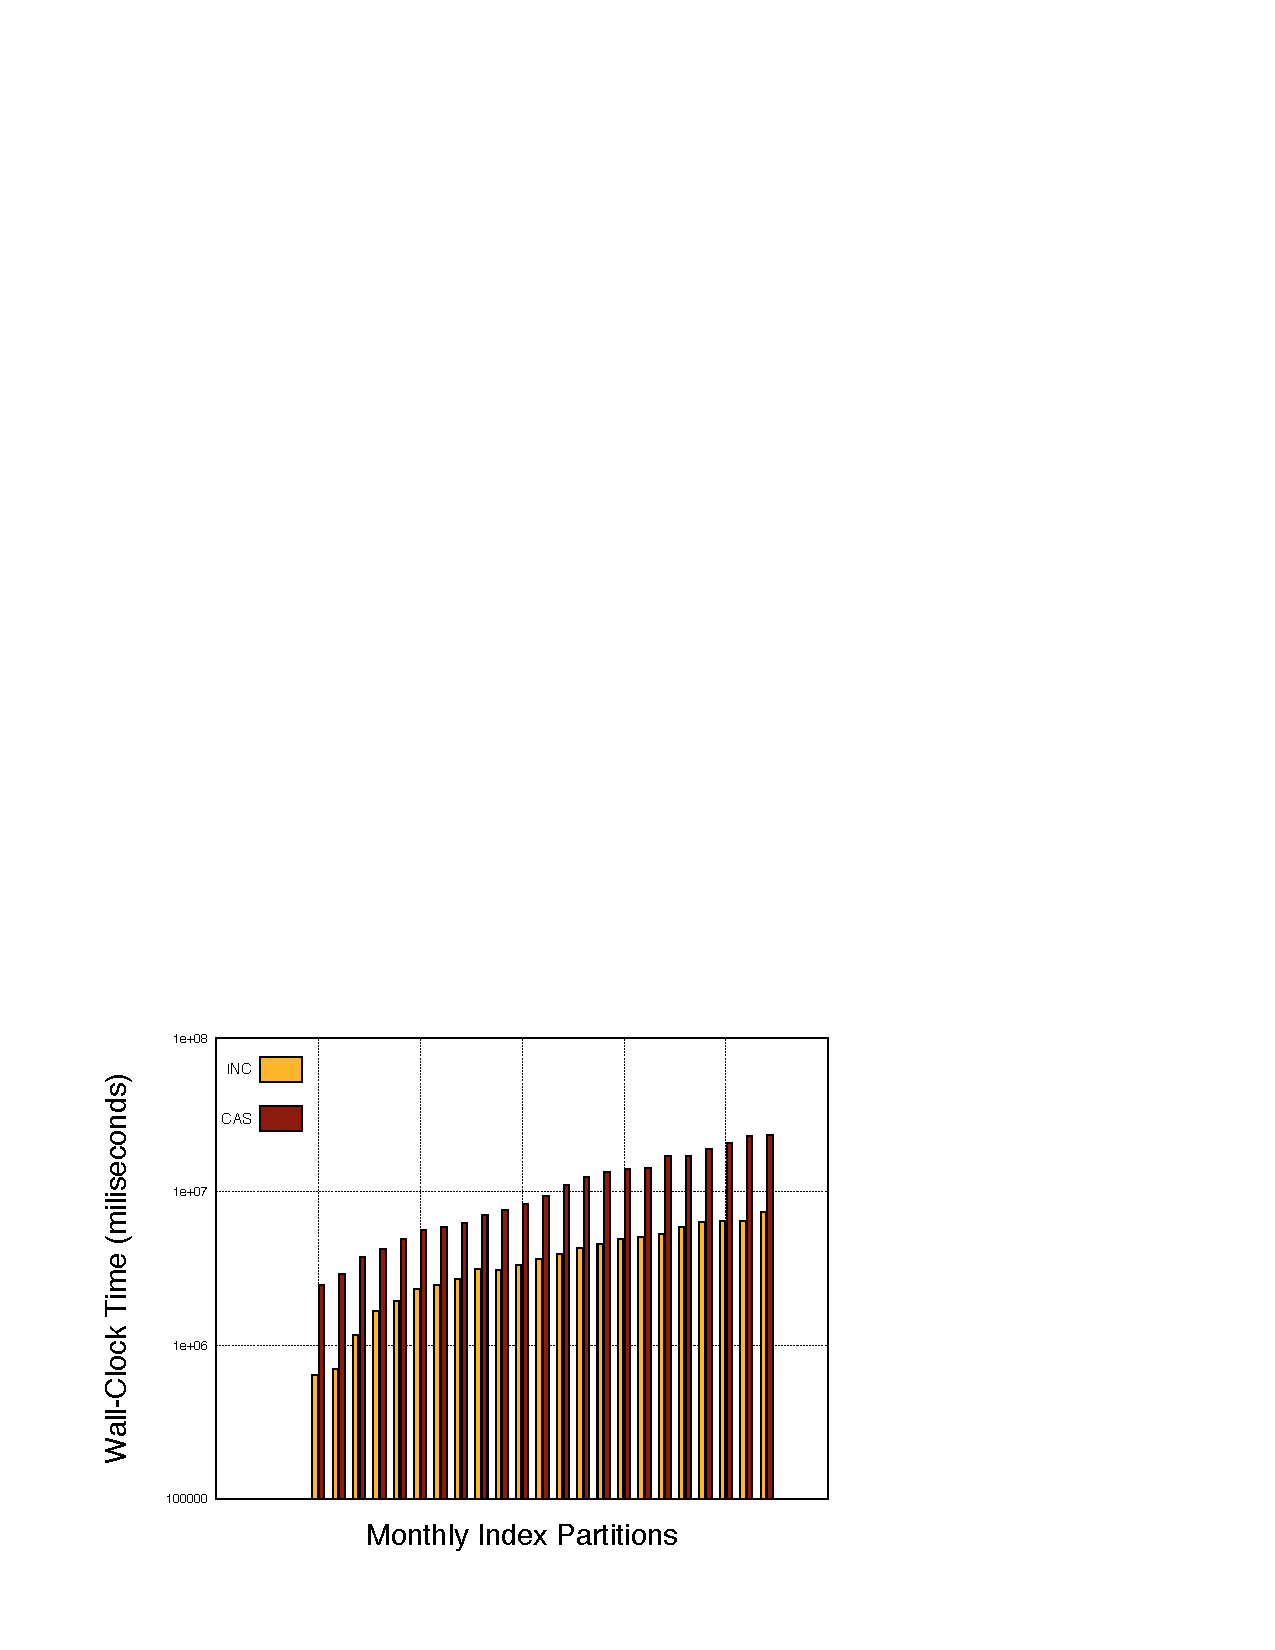
\includegraphics[width=0.6\textwidth]{plots/updates/pdfs/index_maintenance_ukgov_1000.pdf}}
  \caption{Performance of index maintenance -- UKGOV}
  \label{fig:imukgov}
\end{figure*}

\subsection{Index Maintenance Performance}

As we introduced in Section~\ref{chap:sharding:sec:system}, the archive index is maintained by first collecting the updates to a partial-archive index which is then periodically merged into the primary archive index. A partial index is responsible for all versions which end in the time interval between two consecutive merges. To simulate index management for archive indexes as follows: we first created partial indexes for each month containing postings of only those versions that have end time within that month. The index is incrementally maintained, starting from an empty
index, by merging partial indexes of each month in sequence. We employed
\emph{immediate-merging}~\cite{Buttcher:2010fk} to create one
consolidated index at the end of every monthly merge operation, and
each sharded posting list in the index is incrementally maintained
using our incremental sharding algorithm. We compared this with CAS, which
recomputes the entire sharding for the combined index every time from
scratch. In other words, all shards of a posting list in the currently
merged index are read and decompressed, the corresponding list from
the partial index for the next month is also read and decompressed,
these two are combined, and finally, a new sharding is generated using
the CAS algorithm for the merged index, which is finally written in compressed
form to disk.

Figures~\ref{fig:imwiki} and \ref{fig:imukgov} show results of our
experiments on index maintenance with WIKI and UKGOV datasets
respectively. Note the log-scale used on the y-axis,
which represents the time-taken for the consolidated sharded index to
be built in milliseconds. 


It is evident from these charts that INC outperforms CAS by a large margin. In UKGOV, the improvements are nearly a factor of 4 (see Figure~\ref{fig:imukgov}) while the improvements in WIKI are around a factor of 10 (see Figure~\ref{fig:imwiki}).  This efficiency comes from two advantages that INC
enjoys over CAS: first, recomputing the sharding by CA on the merged
index takes much of the time and grows as the index size grows. Since
INC does not recompute the sharding, its performance improves
significantly. Second, it does not have to decompress, merge and shard
the entire list before writing do the disk. Instead, it has to just
read two posting lists in parallel and append corresponding shards
(without decompressing), and write to the disk. From our experiments, we observe that recomputation of shards accounts for an average of 55\%-60\% of the entire maintenance time. Compression and decompression take upto 15\% of the overall time but since we use 7-bit encoding for compression we expect that a more involved compression technique would only increase the maintenance time. It should be noted
that in our simulation we do not perform an append using in-place merge techniques. Instead we resort
to creating a new index file in each step incurring additional
overheads. Thus, the performance of INC can be further improved by
carefully implementing advanced index merging methods.


% \begin{table*}\centering
% \begin{tabular}{@{}lcrcrrcrrccrr@{}}\toprule
% & \multicolumn{1}{c}{\textbf{$\eta=0$}} & \phantom{ab} & \multicolumn{2}{c}{\textbf{$\eta=10$}} & \phantom{ab} & \multicolumn{2}{c}{\textbf{$\eta=100$}}& \phantom{ab} & \multicolumn{2}{c}{\textbf{$\eta=1000$}}\\ 
% \cmidrule{2-2} \cmidrule{4-5} \cmidrule{5-6} \cmidrule{7-8}
%  & IS & CAS & INC && CAS & INC && CAS & INC\\ \midrule
% \textbf{WIKI}\\
%  Day &30 & 17.64 & 15.81 && 11.57 & 10.65 && 11.86 & 8.7\\
%  Month &30 & 29.01 & 28.88 && 25.03 & 24.22 && 24.75 & 22.70\\
%  Year &30 & 131.06 & 132.08 && 127.96 & 125.32 && 127.57 & 123.76\\ 
%  Full &30 & 851.43 & 817.76 && 834.74 & 806.87 && 815.20 & 809.90\\
%  %\textbf{Overall} & - & 51 && 65 & - && - & -\\
% \midrule
% \textbf{UKGOV}\\
%  Day  &30& 55.78 & 50.22 && 53.34 & 44.97 && 49.25 & 43.27\\
%  Month &30& 158.89 & 155.72 && 156.28 & 145.77 && 153.89 & 143.60\\
%  Year  &30& 711.63 & 724.56 && 707.84 & 702.69 && 699.81 & 696.87 \\ 
%  Full  &30& 2875.35 & 2839.80 && 2794.46 & 2845.31 && 2940.5 & 2999.32 \\
%  %\textbf{Overall} & - & 51 && 65 & - && - & -\\
%  \bottomrule
% \end{tabular}
% \caption{Comparison of Wall-clock times between CAS and INC}

% \label{tab:sharding_qp}
% \end{table*}


\section{Related Work}
\label{chap:sharding:sec:related}

Temporal information associated with documents has recently seen
increasing attention in information retrieval. One of the earliest
known efforts in this direction is by Anick and
Flynn~\cite{DBLP:conf/sigir/AnickF92} who developed a framework for
versioning the complete index for historical queries. Recently, Alonso
et al.~\cite{Alonso:2007aa} give an overview of relevant research
directions. The work by Herscovici et
al.~\cite{DBLP:conf/ecir/HerscoviciLY07} focuses on exploiting the
redundancy commonly seen in versioned documents to compress the
inverted index. Similarly, He et al.~\cite{DBLP:conf/cikm/HeYS09,DBLP:conf/cikm/HeZS10} consider the
problem of efficiently storing inverted indexes on disk using
compression; these are orthogonal to our work and could be combined
with our sharding techniques. 

The closest to our work and the most relevant related work is the work on vertical partitioning of posting lists by Berberich et. al.~\cite{kberberi:sigir2007}. They consider posting-list partitioning strategies which trade-off index size and query-processing performance. Two approaches employed by them either bound the index size, called the \emph{space-bound approach}, or bound the worst performance called the \emph{performance-guarantee approach}. Further, they also introduced index compression techniques called temporal coalescing aimed at supporting different query types while keeping the index compact. These compression techniques are also relevant in our setting as shown in our experiments in Section~\ref{expt:coa}.
 
Research in temporal databases has taken a broader perspective beyond
text documents and targeted general class of time-annotated data. 
Index structures tailored to such data like the
Multi-Version B-Tree~\cite{becker1996asymptotically} or LHAM~\cite{Muth2000} are
related to our work, since they also, implicitly or explicitly, rely
on a temporal partitioning and replication of data. It is therefore
conceivable to apply our proposed techniques in conjunction with one
of these index structures.

Work on index maintenance can be categorized into (a) work on maintaining inverted indexes when faced
with changes in the document collection and (b) approaches that make
search aware of temporal information associated with documents. No
work, to the best of our knowledge, has been done at the intersection
of the two categories.

Given that the construction of inverted indexes is well understood and
can easily be parallelized, one existing maintenance strategy has been
to rebuild the index periodically. Returning stale query results, most
of the time, is an obvious disadvantage of this approach. For a long
time, though, this has been the approach taken by major search engines
on the Web. Only lately, Peng et al.~\cite{Peng:2010fk} have addressed
the issue of handling updates in web-scale indexes. Instead of
rebuilding the index, Lester et al.~\cite{lester2006efficient} suggest to
collect updates in an in-memory index that is then merged, from time
to time to amortize costs, with a disk-resident inverted index. This
merge can either be performed in-situ, thus modifying posting lists at
their current location, or by storing entirely new posting lists. A
hybrid approach that chooses between these alternatives is described
by B\"uttcher et al.~\cite{Buttcher:2008fk}. Guarajada and
Kumar~\cite{Gurajada:2009vn} can be seen as another extension that
leverages query logs to determine terms whose posting lists mandate
eager maintenance. In a spirit similar to log-structured
methods~\cite{ONeil:1996fk}, Lester et al.~\cite{Lester:2008qf}
propose to keep multiple indexes of geometrically increasing size and
merge them, when they overflow, in a rolling manner. Query results
reflecting the current state of the document collection can be
obtained in these approaches by executing queries both on in-memory
and disk-resident indexes. For more detailed discussions of inverted
index maintenance we refer the reader to Chapter~\ref{chap:foundations}.

\section{Summary}
\label{chap:sharding:sec:summary}

This chapter presents a novel method of index organization based on
sharding for processing time-travel queries efficiently. Previous approaches traded-off index size and query performance resulting in an index-size blowup. We take an alternative approach of index partitioning by exploiting the valid-intervals and taking into account index-access costs. The resulting index has a small space overhead and we show by experiments that the sharded indexes consistently outperform the vertically-partitioned index in query performance. We also introduce index-maintenance strategies, based on incremental sharding, which avoid expensive shard recomputations when dealing with dynamic collections. We show through experiments that, by employing incremental sharding, we outperform sharding based on recomputation by  at least four times. 
%In the next chapter we address query optimization for time-travel text search. 